% !TEX TS-program = xelatex
% Command for running this example (needs latexmkrc file):
%    latexmk -bibtex -pdf main.tex

%	نمونه پایان‌نامه آماده شده با استفاده از کلاس tehran-thesis، نگارش 1
%	سینا ممکن، دانشگاه تهران 
%	https://github.com/sinamomken/tehran-thesis
%	گروه پارسی‌لاتک
%	http://www.parsilatex.com
%	این نسخه، بر اساس نسخه‌ 0.1 از کلاس IUST-Thesis آقای محمود امین‌طوسی آماده شده است.
%        http://profsite.sttu.ac.ir/mamintoosi

%----------------------------------------------------------------------------------------------
% اگر قصد نوشتن پروژه کارشناسی را دارید، در خط زیر به جای msc، کلمه bsc و اگر قصد نوشتن رساله دکترا را دارید، کلمه phd را قرار دهید. کلیه تنظیمات لازم، به طور خودکار، اعمال می‌شود.

% اگر مایلید پایان‌نامه شما دورو باشد به جای oneside در خط زیر از twoside استفاده کنید.

% برای حاشیه‌نویسی و کم کردن صفحات ابتدایی، گزینه draft را وارد و برای نسخه نهایی آن را حذف کنید.

% برای استفاده از قلم‌های سری IR Series گزینه irfonts را وارد و برای استفاده از قلم‌های X Series 2 آن را حذف کنید.

\documentclass[
oneside
% ,openany
,bsc
,irfonts
% ,draft
]{./tex/tehran-thesis}

% فایل commands.tex را مطالعه کنید؛ چون دستورات مربوط به فراخوانی بسته‌ها، فونت و دستورات خاص در این فایل قرار دارد.
% در این فایل، دستورها و تنظیمات مورد نیاز، آورده شده است.
%-------------------------------------------------------------------------------------------------------------------
% دستوراتی که پوشه پیش‌فرض زیرفایل‌های tex را مشخص می‌کند.
%\makeatletter
%\def\input@path{{./tex/}}
%\makeatother
% در ورژن جدید زی‌پرشین برای تایپ متن‌های ریاضی، این سه بسته، حتماً باید فراخوانی شود
\usepackage{amsthm,amssymb,amsmath}
% بسته‌ای برای تنطیم حاشیه‌های بالا، پایین، چپ و راست صفحه
\usepackage[a4paper, top=40mm, bottom=40mm, outer=25mm, inner=35mm]{geometry}
% بسته‌‌ای برای ظاهر شدن شکل‌ها و تعیین آدرس تصاویر
\usepackage[final]{graphicx}
\graphicspath{{./img/}}
% بسته‌های مورد نیاز برای نوشتن کدها، رنگ‌آمیزی آنها و تعیین پوشهٔ کدها
\usepackage[final]{listings}
\usepackage[usenames,dvipsnames,svgnames,table]{xcolor}
\lstset{inputpath=./code/}
% بسته‌ای برای رسم کادر
\usepackage{framed} 
% بسته‌‌ای برای چاپ شدن خودکار تعداد صفحات در صفحه «معرفی پایان‌نامه»
\usepackage{lastpage}
% بسته‌ٔ لازم برای: ۱. تغییر شماره‌گذاری صفحات پیوست. ۲. تصحیح باگ آدرس وب حاوی '%' در مراجع
\usepackage{etoolbox}

%%%%%%%%%%%%%%%%%%%%%%%%%%%%%%%%%%%%
%%% دستورات وابسته به استیل مراجع:
%% اگر از استیل‌های natbib (plainnat-fa، asa-fa، chicago-fa) استفاده می‌کنید، خط زیر را فعال و بعدی‌اش را غیرفعال کنید.
%\usepackage{natbib}
%\newcommand{\citelatin}[1]{\cite{#1}\LTRfootnote{\citeauthor*{#1}}}
%\newcommand{\citeplatin}[1]{\citep{#1}\LTRfootnote{\citeauthor*{#1}}}
%% اگر از سایر استیل‌ها استفاده می‌کنید، خط بالا را غیرفعال و خط‌های زیر را فعال کنید.
\let\citep\cite
\let\citelatin\cite
\let\citeplatin\cite
%%%%%%%%%%%%
% بررسی حالت پیش نویس
\usepackage{ifdraft}
\ifdraft
{%
	% بسته‌ٔ ایجاد لینک‌های رنگی با امکان جهش
	\usepackage[unicode=true,pagebackref=true,
colorlinks,linkcolor=blue,citecolor=blue,final]{hyperref}
	%\usepackage{todonotes}
	\usepackage[firstpage]{draftwatermark}
	\SetWatermarkText{\ \ \ \rl{پیش‌نویس}}
	\SetWatermarkScale{1.2}
}
{ 
	\usepackage[pagebackref=false]{hyperref}
	%\usepackage[disable]{todonotes} % final without TODOs
}

\usepackage[obeyDraft]{todonotes}
\setlength{\marginparwidth}{2cm}

%%%%%%%%%%%%
%%% تصحیح باگ: اگر در مراجع، آدرس وب حاوی '%' بوده و pagebackref فعال باشد، دستورات زیر باید بیایند:
%% برای استیل‌های natbib مثل plainnat-fa، asa-fa، chicago-fa
\makeatletter
\let\ORIG@BR@@lbibitem\BR@@lbibitem
\apptocmd\ORIG@BR@@lbibitem{\endgroup}{}{}
\def\BR@@lbibitem{\begingroup\catcode`\%=12 \ORIG@BR@@lbibitem}
\makeatother
%% برای سایر استیل‌ها
\makeatletter
\let\ORIG@BR@@bibitem\BR@@bibitem
\apptocmd\ORIG@BR@@bibitem{\endgroup}{}{}
\def\BR@@bibitem{\begingroup\catcode`\%=12 \ORIG@BR@@bibitem}
\makeatother
%%%%%%%%%%%%%%%%%%%%%%%%%%%%%%%%%%%%

% بسته‌ لازم برای تنظیم سربرگ‌ها
\usepackage{fancyhdr}
%\usepackage{enumitem}
\usepackage{setspace}
% بسته‌های لازم برای نوشتن الگوریتم
\usepackage{algorithm}
\usepackage{algorithmic}
% بسته‌های لازم برای رسم بهتر جداول
\usepackage{tabulary}
\usepackage{tabularx}
\usepackage{rotating}
% بسته‌های لازم برای رسم تنظیم بهتر شکل‌ها و زیرشکل‌ها
\usepackage[export]{adjustbox}
\usepackage{subfig}
\usepackage[subfigure]{tocloft}
% بسته‌ای برای رسم نمودارها و نیز صفحه مالکیت اثر
\usepackage{tikz}
% بسته‌ای برای ظاهر شدن «مراجع» و «نماگر» در فهرست مطالب
\usepackage[nottoc]{tocbibind}
% دستورات مربوط به ایجاد نماگر
\usepackage{makeidx}
\makeindex
%%% بسته ایجاد واژه‌نامه با xindy
\usepackage[xindy,toc,acronym,nonumberlist=true]{glossaries}

% بسته‌ای برای افزودن تورفتگی به ابتدای اولین پاراگراف هر بخش
\usepackage{indentfirst}

% بسته زیر باگ ناشی از فراخوانی بسته‌های زیاد را برطرف می‌کند.
\usepackage{morewrites}
%%%%%%%%%%%%%%%%%%%%%%%%%%
% فراخوانی بسته زی‌پرشین (باید آخرین بسته باشد)
\usepackage[extrafootnotefeatures, localise=on, displaymathdigits=persian]{xepersian}




\makeatletter
% تعریف قلم فارسی و انگلیسی و مکان قلم‌ها
\if@irfonts
\settextfont[Path={./font/}, BoldFont={IRLotusICEE_Bold.ttf}, BoldItalicFont={IRLotusICEE_BoldIranic.ttf}, ItalicFont={IRLotusICEE_Iranic.ttf},Scale=1.2]{IRLotusICEE.ttf}
% LiberationSerif or FreeSerif as free equivalents of Times New Roman
\setlatintextfont[Path={./font/}, BoldFont={LiberationSerif-Bold.ttf}, BoldItalicFont={LiberationSerif-BoldItalic.ttf}, ItalicFont={LiberationSerif-Italic.ttf},Scale=1]{LiberationSerif-Regular.ttf}
% چنانچه می‌خواهید اعداد در فرمول‌ها، انگلیسی باشد، خط زیر را غیرفعال کنید
% و گزینهٔ displaymathdigits=persian را از خط ۱۰۹ حذف کنید.
\setdigitfont[Path={./font/}, Scale=1.2]{IRLotusICEE.ttf}
% تعریف قلم‌های فارسی و انگلیسی اضافی برای استفاده در بعضی از قسمت‌های متن
\setiranicfont[Path={./font/}, Scale=1.3]{IRLotusICEE_Iranic.ttf}				% ایرانیک، خوابیده به چپ
\setmathsfdigitfont[Path={./font/}]{IRTitr.ttf}
\defpersianfont\titlefont[Path={./font/}, Scale=1]{IRTitr.ttf}
% برای تعریف یک قلم خاص عنوان لاتین، خط بعد را فعال و ویرایش کنید و خط بعد از آن را غیرفعال کنید.
% \deflatinfont\latintitlefont[Scale=1]{LiberationSerif}
\font\latintitlefont=cmssbx10 scaled 2300 %cmssbx10 scaled 2300
\else
\settextfont{XB Niloofar}
\setlatintextfont{Junicode}
% چنانچه می‌خواهید اعداد در فرمول‌ها، انگلیسی باشد، خط زیر را غیرفعال کنید
% و گزینهٔ displaymathdigits=persian را از خط ۱۰۹ حذف کنید.
\setdigitfont{XB Niloofar}
% تعریف قلم‌های فارسی و انگلیسی اضافی برای استفاده در بعضی از قسمت‌های متن
% \setmathsfdigitfont{XB Titre}
\defpersianfont\titlefont{XB Titre}
\deflatinfont\latintitlefont[Scale=1.1]{Junicode}
\fi
\makeatother

% برای استفاده از قلم نستعلیق خط بعد را فعال کنید.
% \defpersianfont\nastaliq[Scale=1.2]{IranNastaliq}


%%%%%%%%%%%%%%%%%%%%%%%%%%
% راستچین شدن todonotes
\presetkeys{todonotes}{align=right,textdirection=righttoleft}{}
\makeatletter
\providecommand\@dotsep{5}
\def\listtodoname{فهرست کارهای باقیمانده}
\def\listoftodos{\noindent{\Large\vspace{10mm}\textbf{\listtodoname}}\@starttoc{tdo}}
\renewcommand{\@todonotes@MissingFigureText}{شکل}
\renewcommand{\@todonotes@MissingFigureUp}{شکل}
\renewcommand{\@todonotes@MissingFigureDown}{جاافتاده}
\makeatother
% دستوری برای حذف کلمه «چکیده»
% \renewcommand{\abstractname}{}
% دستوری برای حذف کلمه «abstract»
%\renewcommand{\latinabstract}{}
% دستوری برای تغییر نام کلمه «اثبات» به «برهان»
\renewcommand\proofname{\textbf{برهان}}
% دستوری برای تغییر نام کلمه «کتاب‌نامه» به «مراجع»
\renewcommand{\bibname}{واژه نامه}
% دستوری برای تعریف واژه‌نامه انگلیسی به فارسی
\newcommand\persiangloss[2]{#1\dotfill\lr{#2}\\}
% دستوری برای تعریف واژه‌نامه فارسی به انگلیسی 
\newcommand\englishgloss[2]{#2\dotfill\lr{#1}\\}
% تعریف دستور جدید «\پ» برای خلاصه‌نویسی جهت نوشتن عبارت «پروژه/پایان‌نامه/رساله»
\newcommand{\پ}{پروژه/پایان‌نامه/رساله }

%\newcommand\BackSlash{\char`\\}

%%%%%%%%%%%%%%%%%%%%%%%%%%
% \SepMark{-}

% تعریف و نحوه ظاهر شدن عنوان قضیه‌ها، تعریف‌ها، مثال‌ها و ...
\theoremstyle{definition}
\newtheorem{definition}{تعریف}[section]
\theoremstyle{theorem}
\newtheorem{theorem}[definition]{قضیه}
\newtheorem{lemma}[definition]{لم}
\newtheorem{proposition}[definition]{گزاره}
\newtheorem{corollary}[definition]{نتیجه}
\newtheorem{remark}[definition]{ملاحظه}
\theoremstyle{definition}
\newtheorem{example}[definition]{مثال}

%\renewcommand{\theequation}{\thechapter-\arabic{equation}}
%\def\bibname{مراجع}
\numberwithin{algorithm}{chapter}
%\def\listalgorithmname{فهرست الگوریتم‌ها}
\def\listfigurename{فهرست شکل ها}
\def\listtablename{فهرست جدول ها}

% دستور های لازم برای تعریف ترجمهٔ دستورات الگوریتم
\makeatletter
\renewcommand{\algorithmicrequire}{\if@RTL\textbf{ورودی:}\else\textbf{Require:}\fi}
\renewcommand{\algorithmicensure}{\if@RTL\textbf{خروجی:}\else\textbf{Ensure:}\fi}
\renewcommand{\algorithmicend}{\if@RTL\textbf{پایان}\else\textbf{end}\fi}
\renewcommand{\algorithmicif}{\if@RTL\textbf{اگر}\else\textbf{if}\fi}
\renewcommand{\algorithmicthen}{\if@RTL\textbf{آنگاه}\else\textbf{then}\fi}
\renewcommand{\algorithmicelse}{\if@RTL\textbf{وگرنه}\else\textbf{else}\fi}
\renewcommand{\algorithmicfor}{\if@RTL\textbf{برای}\else\textbf{for}\fi}
\renewcommand{\algorithmicforall}{\if@RTL\textbf{برای هر}\else\textbf{for all}\fi}
\renewcommand{\algorithmicdo}{\if@RTL\textbf{انجام بده}\else\textbf{do}\fi}
\renewcommand{\algorithmicwhile}{\if@RTL\textbf{تا زمانی که}\else\textbf{while}\fi}
\renewcommand{\algorithmicloop}{\if@RTL\textbf{تکرار کن}\else\textbf{loop}\fi}
\renewcommand{\algorithmicrepeat}{\if@RTL\textbf{تکرار کن}\else\textbf{repeat}\fi}
\renewcommand{\algorithmicuntil}{\if@RTL\textbf{تا زمانی که}\else\textbf{until}\fi}
\renewcommand{\algorithmicprint}{\if@RTL\textbf{چاپ کن}\else\textbf{print}\fi}
\renewcommand{\algorithmicreturn}{\if@RTL\textbf{بازگردان}\else\textbf{return}\fi}
\renewcommand{\algorithmicand}{\if@RTL\textbf{و}\else\textbf{and}\fi}
\renewcommand{\algorithmicor}{\if@RTL\textbf{و یا}\else\textbf{or}\fi} % TODO add better translate
\renewcommand{\algorithmicxor}{\if@RTL\textbf{یا}\else\textbf{xor}\fi} % TODO add better translate
\renewcommand{\algorithmicnot}{\if@RTL\textbf{نقیض}\else\textbf{not}\fi}
\renewcommand{\algorithmicto}{\if@RTL\textbf{تا}\else\textbf{to}\fi}
\renewcommand{\algorithmicinputs}{\if@RTL\textbf{ورودی‌ها}\else\textbf{inputs}\fi}
\renewcommand{\algorithmicoutputs}{\if@RTL\textbf{خروجی‌ها}\else\textbf{outputs}\fi}
\renewcommand{\algorithmicglobals}{\if@RTL\textbf{متغیرهای عمومی}\else\textbf{globals}\fi}
\renewcommand{\algorithmicbody}{\if@RTL\textbf{انجام بده}\else\textbf{do}\fi}
\renewcommand{\algorithmictrue}{\if@RTL\textbf{درست}\else\textbf{true}\fi}
\renewcommand{\algorithmicfalse}{\if@RTL\textbf{نادرست}\else\textbf{false}\fi}
\renewcommand{\algorithmicendif}{\algorithmicend\textbf{ شرط }\algorithmicif}
\renewcommand{\algorithmicendfor}{\algorithmicend\textbf{ حلقهٔ }\algorithmicfor}
\renewcommand{\algorithmicendwhile}{\algorithmicend\textbf{ حلقهٔ }\algorithmicwhile}
\renewcommand{\algorithmicendloop}{\algorithmicend\textbf{ حلقهٔ }\algorithmicloop}
\renewcommand{\algorithmiccomment}[1]{\{{\itshape #1}\}}
\makeatletter

%%%%%%%%%%%%%%%%%%%%%%%%%%%%
%%% دستورهایی برای سفارشی کردن سربرگ صفحات:
%\newcommand{\SetHeader}[1]{
% دستور زیر معادل با گزینه twoside است.
%\csname@twosidetrue\endcsname
\pagestyle{fancy}
%% دستورات زیر سبک صفحات fancy را تغییر می‌دهد:
% O=Odd, E=Even, L=Left, R=Right
% در صورت oneside بودن، عنوان فصل، سمت چپ ظاهر می‌شود.
\fancyhead{}
\fancyhead[OL]{\small\leftmark}
\fancyhead[ER]{\small\leftmark}
\fancyhead[OR]{\footnotesize\rightmark}
\fancyhead[EL]{\footnotesize\rightmark}
\renewcommand{\headrulewidth}{0.75pt}
% شکل‌دهی شماره و عنوان فصل در سربرگ
\renewcommand{\chaptermark}[1]{\markboth{فصل~\thechapter:\ #1}{}}
\makeatletter
\renewcommand{\rightmark}[1]{\@title}
\makeatother
%}
%%%%%%%%%%%%%%%%%%%%%%%%%%%%
%\def\MATtextbaseline{1.5}
%\renewcommand{\baselinestretch}{\MATtextbaseline}
\doublespacing
%%%%%%%%%%%%%%%%%%%%%%%%%%%%%
% دستوراتی برای اضافه کردن کلمه «فصل» در فهرست مطالب

\newlength\mylenprt
\newlength\mylenchp
\newlength\mylenapp

\renewcommand\cftpartpresnum{\partname~}
\renewcommand\cftchappresnum{\chaptername~}
\renewcommand\cftchapaftersnum{:}

\settowidth\mylenprt{\cftpartfont\cftpartpresnum\cftpartaftersnum}
\settowidth\mylenchp{\cftchapfont\cftchappresnum\cftchapaftersnum}
\settowidth\mylenapp{\cftchapfont\appendixname~\cftchapaftersnum}
\addtolength\mylenprt{\cftpartnumwidth}
\addtolength\mylenchp{\cftchapnumwidth}
\addtolength\mylenapp{\cftchapnumwidth}

\setlength\cftpartnumwidth{\mylenprt}
\setlength\cftchapnumwidth{\mylenchp}	

\makeatletter
{\def\thebibliography#1{\chapter*{\refname\@mkboth
   {\uppercase{\refname}}{\uppercase{\refname}}}\list
   {[\arabic{enumi}]}{\settowidth\labelwidth{[#1]}
   \rightmargin\labelwidth
   \advance\rightmargin\labelsep
   \advance\rightmargin\bibindent
   \itemindent -\bibindent

   \listparindent \itemindent
   \parsep \z@
   \usecounter{enumi}}
   \def\newblock{}
   \sloppy
   \sfcode`\.=1000\relax}}
   
%اگر مایلید در شماره گذاری حرفی و ابجد به جای آ از الف استفاده شود دستورات زیر را فعال کنید.   
%\def\@Abjad#1{%
%  \ifcase#1\or الف\or ب\or ج\or د%
%           \or هـ\or و\or ز\or ح\or ط%
%           \or ی\or ک\or ل\or م\or ن%
%           \or س\or ع\or ف\or ص%
%           \or ق\or ر\or ش\or ت\or ث%
%            \or خ\or ذ\or ض\or ظ\or غ%
%            \else\@ctrerr\fi}
%
% \def\abj@num@i#1{%
%   \ifcase#1\or الف\or ب\or ج\or د%
%            \or هـ‍\or و\or ز\or ح\or ط\fi

%   \ifnum#1=\z@\abjad@zero\fi}   
%  
%   \def\@harfi#1{\ifcase#1\or الف\or ب\or پ\or ت\or ث\or

% ج\or چ\or ح\or خ\or د\or ذ\or ر\or ز\or ژ\or س\or ش\or ص\or ض\or ط\or ظ\or ع\or غ\or

% ف\or ق\or ک\or گ\or ل\or م\or ن\or و\or ه\or ی\else\@ctrerr\fi}

%
\makeatother

%%% امکان درج کد در سند
% در این قسمت رنگ، قلم و قالب‌بندی قسمت‌های مختلف یک کد تعیین می‌شود. 
\lstdefinestyle{myStyle}{
	basicstyle=\ttfamily, % whole listing /w verbatim font
	keywordstyle=\color{blue}\bfseries, % bold black keywords
	identifierstyle=, % nothing happens
	commentstyle=\color{LimeGreen}, % green comments
	stringstyle=\ttfamily\color{red}, % red typewriter font for strings
	showstringspaces=false % no special string spaces
	breaklines=true,
	breakatwhitespace=false,
	numbers=right, % line number formats
	numberstyle=\footnotesize\lr,
	numbersep=-10pt,
	frame=single,
	captionpos=b,
	captiondirection=RTL
}
\lstset{style=myStyle} % command to set default style
\def\lstlistingname{\rl{برنامهٔ}}
% \def\lstlistlistingname{\rl{فهرست برنامه‌ها}}


% for numbering subsubsections
\setcounter{secnumdepth}{3}
%to include subsubsections in the table of contents
\setcounter{tocdepth}{3}

\makeatletter
\renewcommand{\p@subfigure}{\thefigure.}
\makeatother


% مشخصات پایان‌نامه را در فایلهای faTitle و enTitle وارد نمایید.
% !TeX root=../main.tex
% در این فایل، عنوان پایان‌نامه، مشخصات خود، متن تقدیمی‌، ستایش، سپاس‌گزاری و چکیده پایان‌نامه را به فارسی، وارد کنید.
% توجه داشته باشید که جدول حاوی مشخصات پروژه/پایان‌نامه/رساله و همچنین، مشخصات داخل آن، به طور خودکار، درج می‌شود.
%%%%%%%%%%%%%%%%%%%%%%%%%%%%%%%%%%%%
% دانشگاه خود را وارد کنید
\university{دانشگاه اصفهان}
% دانشکده، آموزشکده و یا پژوهشکده  خود را وارد کنید
\faculty{دانشکده مهندسی کامپیوتر}
% گروه آموزشی خود را وارد کنید (در صورت نیاز)
\department{گروه مهندسی نرم افزار}
% رشته تحصیلی خود را وارد کنید
\subject{مهندسی نرم افزار}
% گرایش خود را وارد کنید

% عنوان پایان‌نامه را وارد کنید
\title{ارتقای سيستم گفتگوی وظيفه گرا از طریق تنظيم سریع و نماگر سازی کاربر}
% نام استاد راهنما را وارد کنید
\firstsupervisor{دکتر افسانه فاطمی}
\firstsupervisorrank{استاد}

% نام داور خود را وارد نمایید.
\internaljudge{دکتر داور داخلی}
\internaljudgerank{دانشیار}

% نام دانشجو را وارد کنید
\name{عارف}
% نام خانوادگی دانشجو را وارد کنید
\surname{یزدخواستی}
% شماره دانشجویی دانشجو را وارد کنید
\studentID{4013644018}
% تاریخ پایان‌نامه را وارد کنید
\thesisdate{فروردین 1404}
% به صورت پیش‌فرض برای پایان‌نامه‌های کارشناسی تا دکترا به ترتیب از عبارات «پروژه»، «پایان‌نامه» و «رساله» استفاده می‌شود؛ اگر  نمی‌پسندید هر عنوانی را که مایلید در دستور زیر قرار داده و آنرا از حالت توضیح خارج کنید.
%\projectLabel{پایان‌نامه}

% به صورت پیش‌فرض برای عناوین مقاطع تحصیلی کارشناسی تا دکترا به ترتیب از عبارت «کارشناسی»، «کارشناسی ارشد» و «دکتری» استفاده می‌شود؛ اگر نمی‌پسندید هر عنوانی را که مایلید در دستور زیر قرار داده و آنرا از حالت توضیح خارج کنید.
%\degree{}
%%%%%%%%%%%%%%%%%%%%%%%%%%%%%%%%%%%%%%%%%%%%%%%%%%%%
%% پایان‌نامه خود را تقدیم کنید! %%
\dedication
{
	{\Large تقدیم به:}\\
	\begin{flushleft}{
			\huge
			خانواده که همواره پشتم و همه دردهایم را مرهم هستند\\
		}
	\end{flushleft}
}
%% متن قدردانی %%
%% ترجیحا با توجه به ذوق و سلیقه خود متن قدردانی را تغییر دهید.
\acknowledgement{
	سپاس و آفرین خداوندگار جان آفرین راست ، اوی که آدمی را به گوهر خرد آراست.
	
	در آغاز دستان پدر و مادر نازنینم را به پاس مهر بیکرانشان به گرمی می فشارم، 
	و از استاد راهنما خود سرکار خانم دکتر افسانه فاطمی بابت زمان و انرژی‌ای که گذاشتند سپاس گزاری می‌کنم.
	
	
	و در پایان، سپاس گزاری می کنم از همه اعضای خانواده دانشکده مهندسی کامپیوتر اصفهان به ویژه دوستانم که بهترین روزهای زندگی من را رقم زدند.
}

%%%%%%%%%%%%%%%%%%%%%%%%%%%%%%%%%%%%
%چکیده پایان‌نامه را وارد کنید
\fa-abstract{

سیستم‌های گفتگوی وظیفه‌گرا% 
\LTRfootnote{Task-oriented dialogue system (TODS)}
نقش محوری در ارائه خدمات شخصی‌سازی‌شده از طریق تعاملات انسان و هوش مصنوعی ایفا می‌کنند. با این حال، این سیستم‌ها با چالش‌های مهمی از جمله شخصی‌سازی ناکافی، مشکل شروع سرد%
\LTRfootnote{Cold start}
 و نگرانی‌های مربوط به حریم خصوصی مواجه هستند. این مسائل مانع از توانایی آنها در ارائه تجربیات کاربری یکپارچه و قابل اعتماد می‌شود. علاوه بر این، داده‌های محدود کاربر اغلب دشواری ایجاد تعاملات شخصی‌سازی‌شده مؤثر را تشدید می‌کند، در حالی که عدم رعایت مقررات جهانی حریم خصوصی، استقرار آنها را پیچیده‌تر می‌کند.
برای پرداختن به این چالش‌ها، ما یک رویکرد جدید تحت عنوان "MindMeld" پیشنهاد می‌کنیم که تکنیک‌های پیشرفته‌ای را برای شخصی‌سازی، نماگرکاربر%
\LTRfootnote{User profiling}
 و حفظ حریم خصوصی ادغام می‌کند. این سیستم از تنظیم سریع%
\LTRfootnote{Prompt-tuning}
 مدل‌های زبانی بزرگ برای انطباق سریع با نیازهای خاص کاربر، حتی در سناریوهایی با داده‌های محدود، بهره می‌برد. این سیستم شامل فیلتر مشارکتی مبتنی بر آیتم%
\LTRfootnote{Item-based collaborative filtering}
 است که با تحلیل احساسات%
\LTRfootnote{Semantic analysis}
 بهبود یافته است تا بر مشکل شروع سرد غلبه کند و دقت توصیه را بهبود بخشد. علاوه بر این، MindMeld حق فراموش شدن%
\LTRfootnote{The right to be forgotton}
 را پیاده‌سازی می‌کند و کاربران را قادر می‌سازد تا داده‌های خود را بدون به خطر انداختن عملکرد سیستم، به صورت پویا حذف کنند. این امر انطباق با استانداردهای جهانی حریم خصوصی را تضمین می‌کند و اعتماد کاربر را افزایش می‌دهد. با ترکیب یادگیری چندشات%
\LTRfootnote{Few-shot learning}
 با تنظیم سریع، سیستم حتی در محیط‌های با کمبود داده، به عملکرد قوی دست می‌یابد.
اثربخشی MindMeld با استفاده از معیارهای جامع، از جمله پیچیدگی%
\LTRfootnote{Perplexity}
، تمایز%
\LTRfootnote{Distinct}
، میزان موفقیت%
\LTRfootnote{Success rate}
، نرخ تکمیل کار%
\LTRfootnote{Completion rate}
 و امتیاز تعامل کاربر%
\LTRfootnote{User engagement score}
ارزیابی شد. نتایج، پیشرفت‌هایی را نسبت به رویکردهای موجود نشان می‌دهد. به طور خاص، میزان موفقیت در مقایسه با مطالعات مشابه ۱۷٪ افزایش یافته و تمایز ۱۲٪ بهبود یافته است. این یافته‌ها، توانایی سیستم را در ارائه تعاملات شخصی‌سازی شده و کارآمد، ضمن حفظ حریم خصوصی و اعتماد کاربر، برجسته می‌کند. به طور کلی، MindMeld یک راه حل مقیاس‌پذیر و اخلاقی برای سیستم‌های گفتگوی وظیفه محور ارائه می‌دهد و شکاف‌هایی در شخصی‌سازی، حریم خصوصی و قابلیت استفاده را پر می‌کند.

% کلمات کلیدی پایان‌نامه را وارد کنید
}
\keywords{سیستم گفتگوی وظیفه‌گرا، نماگر کاربری، حق فراموشی، تنظیم سریع، فیلتر مشارکتی}



%%%%%%%%%%%%%%%%%%%%%%%%%%%%%%%%%%%%
% %چکیده پایان‌نامه را وارد کنید
\en-abstract{
\begin{flushleft}
\begin{LTR}

Task-oriented dialogue systems play a central role in delivering personalized services through human-AI interactions. However, these systems face significant challenges, including insufficient personalization, the cold start problem, and privacy concerns. These issues hinder their ability to deliver seamless and reliable user experiences. Furthermore, limited user data often exacerbates the difficulty of creating effective personalized interactions, while lack of compliance with global privacy regulations complicates their deployment. To address these challenges, we propose an approach, named "MindMeld,” that integrates advanced techniques for personalization, user profiling, and privacy. The system leverages prompt-tuning of large language models to quickly adapt to specific user needs, even in data-limited scenarios. The system includes item-based collaborative filtering, enhanced with sentiment analysis to overcome the cold start problem and improve recommendation accuracy. In addition, MindMeld implements the right to be forgotten, enabling users to dynamically delete their data without compromising system performance. This ensures compliance with global privacy standards and increases user trust. By combining few-shot learning with rapid tuning, the system achieves robust performance even in data-poor environments. The effectiveness of MindMeld was evaluated using comprehensive metrics, including Perplexity, Distinct, Success rate, Completion rate, and User engagement score. The results show improvements over existing approaches. Specifically, the success rate increased by seventeen percent and Distinction improved by twelve percent compared to similar studies. These findings highlight the system’s ability to deliver personalized and efficient interactions while maintaining user privacy and trust. Overall, MindMeld provides a scalable and ethical solution for task-based conversational systems, bridging gaps in personalization, privacy, and usability.

\vspace{1cm}
\textbf{Keywords:}  Task-oriented dialogue system (TODS), User Profile, Right To Be Forgotten, Prompt-tuning, Collaborative Filtering.


\end{LTR}
\end{flushleft}
}




% انتهای وارد کردن فیلد‌ها
%%%%%%%%%%%%%%%%%%%%%%%%%%%%%%%%%%%%%%%%%%%%%%%%%%%%%%



% تنظیمات و تعاریف واژه‌نامه و اختصارات
\input{./tex/glossaries-settings}
\input{./tex/words}
\input{./tex/acronyms}


%reset number of foot notes for each page
\usepackage{everypage}
\renewcommand{\footnoterule}{\vspace{1em}\hrule width \linewidth height 0.5pt}
\AddEverypageHook{\setcounter{footnote}{0}}

\usepackage{graphicx}
\usepackage{array}
\usepackage{xepersian} % RTL support and Persian fonts
\usepackage{tabularx}
\usepackage{setspace} % For \onehalfspacing
\usepackage{fontawesome} % For speical chars like check and Cross

\usepackage{cite} % for numbered citations
\usepackage{setspace} % for one-and-a-half spacing
\usepackage{url} % for URLs in bibliography
 
\usepackage{hyperref} %for hyperlinking

\usepackage{csquotes} %for custom quoting
\usepackage{bidi} %for LTR support
\usepackage{amsmath} % For mathematical symbols
\usepackage{bidi}       % For bidirectional support
\usepackage{amsmath} % if you're using math environments
\usepackage{xepersian}



\begin{document}
\nocite{*} % This includes all references in the .bib file

\pagenumbering{adadi} % یک، دو، ...
\besmPage
\titlePage
\davaranPage
%%%%%%%%%%%%%%%%%%%%%%%%%%%
  
    \taghdimPage
    \ghadrdaniPage

\persianAbstractPage
% شروع درج فهرست‌ها
\newpage\cleardoublepage
\pagenumbering{harfi} % آ، ب، ...
\tableofcontents \clearpage
% بررسی حالت پیش‌نویس برای بقیه فهرست‌ها
\ifoptiondraft{
    \listoftodos
}{%
    \listoffigures \clearpage
    \listoftables
    % \addcontentsline{toc}{chapter}{\listalgorithmname}
    % \listofalgorithms \clearpage
    % \addcontentsline{toc}{chapter}{\lstlistlistingname}
    % \lstlistoflistings \clearpage
    \printacronyms
} % end ifoptiondraft

\pagestyle{fancy}
\pagenumbering{arabic} % 1, 2, ...

% !TeX root=../main.tex

\chapter{پیش گفتار}

\section{مقدمه}

سیستم‌های گفتگوی وظیفه‌گرا%
\LTRfootnote{Task-Oriented Dialogue System}
 به عنوان یکی از مهم‌ترین ابزارهای تعامل انسان و ماشین، نقش اساسی در بهبود تجربه کاربری در حوزه‌هایی مانند سیستم‌های توصیه‌گر، خدمات مشتری و تجارت الکترونیک ایفا می‌کنند \cite{camilleri2024artificial}. این سیستم‌ها با درک پرسش‌های کاربران و ارائه پاسخ‌های متناسب، تجربه‌ای طبیعی‌تر و مؤثر را در تعاملات کاربران با سیستم فراهم می‌کنند 
\cite{bocklisch2024task}. 

سیستم‌های گفتگوی وظیفه‌گرا به نوعی از سیستم‌های هوش مصنوعی اطلاق می‌شود که به منظور کمک به کاربران در انجام یک وظیفه خاص طراحی شده‌اند. این وظایف معمولاً شامل ارائه اطلاعات، انجام خدمات یا حل مشکلات عملی است. این سیستم‌ها با استفاده از تعاملات چندمرحله‌ای، به کاربران کمک می‌کنند تا به نتیجه مطلوب برسند، مانند رزرو بلیط، پیدا کردن اطلاعات مربوط به محصولات یا حتی ارائه پیشنهادات شخصی‌سازی شده. 

تفاوت اصلی این سیستم‌ها با سیستم‌های گفتگوی عمومی در این است که آنها بر حل وظایف خاص و عملی متمرکز هستند و تعاملات آنها همواره با هدف دستیابی به یک نتیجه مشخص هدایت می‌شوند. به عبارت دیگر، این سیستم‌ها بر اساس وظیفه خاص خود عمل می‌کنند و هر مرحله از گفتگو به صورت دقیق و هدفمند طراحی شده است تا کاربر را به سمت تکمیل وظیفه هدایت کنند.

از ویژگی‌های اصلی سیستم‌های گفتگوی وظیفه‌گرا می توان به تمرکز بر وظایف عملی اشاره کرد. این سیستم‌ها بر انجام وظایف مشخص مانند رزرو هتل، سفارش غذا یا پاسخ به سؤالات فنی تمرکز دارند. همچنین این سیستم ها شامل تعامل چندمرحله‌ای هستند که معمولاً شامل چندین مرحله از گفتگو هستند که در هر مرحله اطلاعات جدیدی از کاربر دریافت می‌شود و بر اساس آن تصمیم‌گیری می‌شود. علاوه بر موارد ذکرشده این سیستم‌ها اغلب از داده‌های کاربر (مانند ترجیحات یا سابقه تعاملات) استفاده می‌کنند تا پاسخ‌ها و پیشنهادات دقیق‌تری ارائه دهند.
\cite{samarinas2024simulating}

با این حال، چالش‌های زیادی از جمله نیاز به تنظیم دقیق مدل‌های زبانی، شخصی‌سازی پاسخ‌ها بر اساس ترجیحات کاربران، مشکل شروع سرد برای کاربران جدید و نگرانی‌های مربوط به حریم خصوصی همچنان به عنوان موانع اصلی در مسیر پیشرفت این فناوری‌ها مطرح هستند 
\cite{yuan2023user}.

یکی از مهم‌ترین چالش‌های این حوزه، شخصی‌سازی پاسخ‌ها و انطباق‌پذیری سیستم با نیازهای خاص هر کاربر است. در بسیاری از روش‌های موجود، اطلاعات کاربر به صورت ایستا در سیستم ذخیره می‌شود، اما عدم تطبیق آن با تغییرات در رفتار و سلیقه کاربران باعث کاهش دقت توصیه‌ها و کاهش رضایت کاربر به مرور زمان می‌شود 
\cite{azzam2022model}. 

علاوه بر این، مشکل شروع سرد، یعنی ناتوانی سیستم در ارائه پاسخ‌های دقیق به کاربران جدید که سابقه‌ای در سیستم ندارند، یکی از مسائل جدی در سیستم‌های توصیه‌گر و گفتگوی وظیفه‌گرا است
 \cite{yuan2023user}. 
از سوی دیگر، حفظ حریم خصوصی کاربران یکی دیگر از چالش‌های کلیدی در این زمینه است؛ کاربران نیاز دارند که داده‌هایشان در صورت درخواست حذف شود، اما بسیاری از روش‌های سنتی قابلیت اجرایی مؤثری در این زمینه ندارند
 \cite{zhang2024right}.

در کنار این چالش‌ها، روش‌های تنظیم دقیق مدل‌های زبانی، اگرچه باعث بهبود عملکرد سیستم‌های گفتگوی وظیفه‌گرا می‌شوند، اما به دلیل نیاز به منابع محاسباتی بسیار بالا و زمان طولانی پردازش، محدودیت‌هایی را ایجاد می‌کنند 
\cite{kasahara2022building}. 
علاوه بر این، روش‌های سنتی تنظیم دقیق معمولاً نیازمند حجم وسیعی از داده‌های آموزش هستند که در بسیاری از موارد به‌راحتی در دسترس نیستند. به همین دلیل، در سال‌های اخیر استفاده از روش تنظیم سریع%
\LTRfootnote{Prompt-Tuning}
 مورد توجه قرار گرفته است، چرا که این روش بدون نیاز به تغییر تمام پارامترهای مدل، امکان انطباق سریع‌تر و مؤثرتر را با دامنه‌های خاص فراهم می‌کند 
\cite{madotto2021few}.

تنظیم سریع یک روش نوین در بهینه‌سازی مدل‌های زبانی بزرگ است که به جای تغییر کلی پارامترهای مدل، تنها ورودی‌های مدل را تنظیم می‌کند. این رویکرد با افزودن یک لایه سبک‌وزن به مدل پیش‌آموزش‌دیده، به آن اجازه می‌دهد تا برای وظایف خاص تنظیم شود. به عبارت دیگر، تنظیم سریع به این معناست که مدل بدون تغییر در ساختار داخلی خود، با استفاده از ورودی‌های بهینه‌شده، عملکرد بهتری در حوزه‌های خاص ارائه دهد.

تنظیم دقیق شامل تغییر کلی پارامترهای مدل است، که منجر به تنظیم عمیق‌تر می‌شود. اما تنظیم سریع تنها ورودی‌های مدل (مانند پرامپت‌ها) را تنظیم می‌کند و ساختار داخلی مدل را دست‌نخورده باقی می‌گذارد. 

همچنین تنظیم دقیق به دلیل نیاز به به‌روزرسانی تمام پارامترهای مدل، منابع محاسباتی بسیار بالایی مصرف می‌کند ولی تنظیم سریع به دلیل تمرکز بر تنظیم ورودی‌ها، هزینه محاسباتی کمتری دارد و قابلیت استفاده در محیط‌های با منابع محدود را فراهم می‌کند.

علاوه بر آن تنظیم دقیق معمولاً به حجم بالایی از داده‌های آموزشی نیاز دارد ولی تنظیم سریع قادر است با استفاده از داده‌های کم هم عملکرد قابل قبولی ارائه دهد% 
\cite{wang2022no}.

از مزایای تنظیم سریع می توان به سرعت و کارایی بالا اشاره کرد. تنظیم سریع به دلیل عدم نیاز به تغییر کلی پارامترهای مدل، سرعت بیشتری در فرآیند تنظیم دارد و منابع محاسباتی کمتری مصرف می‌کند.
علاه بر آن تنظیم سریع عملکرد عمومی مدل را حفظ می کند. از آنجایی که تنظیم سریع ساختار داخلی مدل را تغییر نمی‌دهد، عملکرد عمومی مدل در وظایف دیگر حفظ می‌شود.
همچنین تنظیم سریع برای سناریوهایی که داده‌های آموزشی محدود هستند (مانند مشکل شروع سرد) بسیار مؤثر است. لازم به ذکر است که این روش به راحتی قابل استفاده در حوزه‌های مختلفی مانند سیستم‌های گفتگوی وظیفه‌گرا و سیستم‌های توصیه‌گر است% 
\cite{kasahara2022building}.
.



این پژوهش با هدف ارائه یک چارچوب جدید برای بهبود سیستم‌های گفتگوی وظیفه‌گرا، ترکیبی از تکنیک‌های تنظیم سریع و نماگر‌سازی پویا را پیشنهاد می‌دهد. در این روش، ابتدا داده‌های مرتبط با کاربر از طریق ترکیب حلیل احساسات برچسب‌های کاربر، فیلتر مشارکتی مبتنی بر آیتم، و تحلیل بازخورد کاربر استخراج شده و سپس با استفاده از تکنیک‌های تنظیم سریع و با استفاده از قدرت مدل های زبانی برای پاسخ‌گویی دقیق‌تر و شخصی‌سازی‌شده تنظیم می‌شود 
\cite{elahi2023hybrid}. 
این سیستم همچنین امکان حذف داده‌های کاربر را مطابق با حق فراموشی فراهم می‌کند تا از حریم خصوصی کاربران محافظت شود 
\cite{zhang2024right}.

با توجه به این رویکرد نوآورانه، انتظار می‌رود که نتایج این تحقیق بتواند راه را برای پیشرفت‌های آینده در حوزه شخصی‌سازی سیستم‌های گفتگوی وظیفه‌گرا هموار کند و الگویی برای بهبود تعاملات کاربر-ماشین در حوزه‌های مختلف از جمله تجارت الکترونیک، خدمات مشتریان، و سیستم‌های یادگیری هوشمند فراهم آورد 
\cite{chen2023zero}.

\section{بیان مسئله}
تحقیقات موجود در حوزه سیستم‌های گفتگوی وظیفه‌گرا به رغم پیشرفت‌های چشمگیر، همچنان دارای کاستی‌هایی هستند:
\begin{itemize}
\item
نبود تمرکز بر حفظ حریم خصوصی کاربران: بسیاری از سیستم‌های موجود داده‌های کاربر را بدون امکان حذف یا اصلاح ذخیره می‌کنند، که می‌تواند منجر به نگرانی‌های امنیتی و اخلاقی شود.
\item
نماگر‌سازی ناکارآمد: روش‌های موجود در نماگر‌سازی کاربران اغلب تنها به استفاده از یک تکنیک محدود هستند و از روش هایی مانند بازخورد موثر کاربران و نماگر پویا برای به‌روزرسانی مدل‌ها استفاده نمی‌کنند.
\item
نیاز به منابع سخت‌افزاری قدرتمند: تنظیم دقیق مدل‌های زبانی به منابع عظیم سخت‌افزاری نیاز دارد که اجرای آن را برای بسیاری از کاربران و سازمان‌ها دشوار می‌کند.
\end{itemize}

روش‌های متعددی با استفاده از متدهای مختلف هم با و هم بدون استفاده از مدل‌های زبانی طی سال ‌های اخیر ارایه شده است اما آنها نیز دارای کاستی‌هایی در کار خود هستند:
\begin{itemize}
\item
نبود تنوع در روش‌های نماگر‌سازی: تحقیقات فعلی عمدتاً به یک رویکرد محدود می‌شوند، در حالی که ترکیب روش‌های مختلف می‌تواند به دقت بیشتری در شخصی‌سازی پاسخ‌ها منجر شود که در نهایت به بهبود سیستم و افزایش کیفیت مکالمه و رضایت کاربر منجر می شوند.
\item
مشکلات شروع سرد: سیستم‌های موجود در مواجهه با کاربران جدید یا داده‌های ناکافی، عملکرد ضعیفی دارند.
\item
عدم امکان تنظیم سریع: بیشتر تحقیقات به تنظیم دقیق مدل وابسته هستند که نه تنها زمان‌بر و پرهزینه است، بلکه انعطاف‌پذیری کمتری نسبت به تنظیم سریع دارد.
\item
عدم رعایت حق فراموشی: کاربران نمی‌توانند داده‌های خود را حذف یا به‌روزرسانی کنند، که این مسئله اعتماد به سیستم را کاهش می‌دهد.
\end{itemize}


\section{اهداف پژوهش}

اهداف پژوهش باید منعکس‌کننده چالش‌های اصلی، گپ‌های موجود در ادبیات، و راه‌حل‌هایی باشد که تحقیق حاضر ارائه می‌دهد. 

هدف از اين تحقیق ارائه روشی مبتنی بر استفاده از تکنیکهای تنظیم سريع به همراه پروفايل سازی کاربر جهت ارتقای سیستم های گفتگوی وظیفه گرا و بهبود آنها است.


\section{فرضیه‌های پژوهش}


فرضیه اصلی پژوهش به صورت زیر است.

استفاده از روش ترکیبی نماگر‌سازی کاربر به همراه تنظیم سریع در سیستم‌های گفتگوی وظیفه‌گرا می‌تواند به طور موثری منجر به ارتقای عملکرد آن‌ها در پاسخگویی به نیازهای کاربران گردد.

این فرضیه به صورت مستقیم به بررسی نحوه استفاده از نماگر کاربر و تنظیم سریع برای بهبود معیارهایی چون رضایت کاربر، تعامل، و دقت پاسخ‌ها می‌پردازد. ترکیب این دو روش، با رویکردی جامع‌تر، مشکلاتی نظیر شروع سرد، حریم خصوصی و تعاملات بلندمدت کاربر را هدف قرار می‌دهد.


\section{سوال‌های پژوهش}

در این بخش، سوالات پژوهش بیان شده است. این فرضیات مبتنی بر شکاف‌های موجود در ادبیات پژوهشی و نیازهای سیستم‌های گفتگوی وظیفه‌گرا تدوین شده‌اند.

\begin{enumerate}
\item
استفاده از تنظیم سریع به چه صورت می‌تواند منجر به ارتقای سیستم گفتگوی وظیفه‌گرا شود؟

\item
استفاده از داده‌های نماگر کاربر در سیستم‌های گفتگوی وظیفه‌گرا از چه راه‌هایی بر رفتار و تعامل کاربر تأثیر می‌گذارد و چگونه می‌توان از این اطلاعات برای بهبود عملکرد کلی سیستم گفتگو استفاده کرد؟

\item
چه ویژگی‌ها و شاخص‌هایی باید در نماگر‌سازی کاربر در سیستم‌های گفتگوی وظیفه‌گرا مورد توجه قرار گیرند؟
\end{enumerate}

\section{نوآوری‌ها و سهم پژوهش}
در این بخش، نوآوری‌ها و سهم علمی پژوهش حاضر با توجه به دستاوردهای اصلی و ایده‌های منحصربه‌فرد آن ارائه می‌شود.
\begin{enumerate}
\item
معرفی رویکرد ترکیبی تنظیم سریع و نماگر‌سازی کاربر

یکی از مهم‌ترین نوآوری‌های پژوهش حاضر، معرفی یک رویکرد ترکیبی است که از تنظیم سریع و نماگر‌سازی پیشرفته کاربر بهره می‌برد. این رویکرد نشان می‌دهد که چگونه تلفیق داده‌های شخصی‌سازی‌شده با تنظیم سریع می‌تواند به بهبود پاسخ‌دهی و رضایت کاربر منجر شود. در این راستا، یک مدل مفهومی برای ادغام داده‌های کاربر و تنظیم سریع ارائه شده است که قابلیت استفاده در دیگر حوزه‌های سیستم‌های توصیه‌گر را نیز دارد. این رویکرد به طور خاص در شرایطی که داده‌های کاربر محدود است، مانند مشکل شروع سرد ، عملکرد بهتری از خود نشان می‌دهد.

\item
تاکید بر حریم خصوصی کاربران از طریق پیاده‌سازی حق فراموشی

پژوهش حاضر با ارائه مکانیزمی برای حذف داده‌های کاربران، به مسئله حفظ حریم خصوصی به صورت جدی پرداخته است. حق فراموشی به کاربران اجازه می‌دهد داده‌های خود را به صورت پویا حذف کنند بدون اینکه عملکرد کلی سیستم تحت تأثیر قرار گیرد. این رویکرد نه تنها اعتماد کاربر را افزایش می‌دهد، بلکه با قوانین جهانی حفظ حریم خصوصی هماهنگ است . این موضوع به عنوان یکی از نوآوری‌های پژوهش شناخته می‌شود که در ادبیات پیشین به ندرت مورد توجه قرار گرفته است.

\item
حل مشکلات شروع سرد با رویکردهای متنوع

مشکل شروع سرد یکی از چالش‌های سیستم‌های توصیه‌گر و گفتگوی وظیفه‌گرا است. این پژوهش با استفاده از ترکیبی از رویکردهای مختلف مانند فیلتر مشارکتی مبتنی بر آیتم و تحلیل احساسات، به حل این مشکل پرداخته است. به عنوان مثال، از تحلیل احساسات برای استخراج علایق کاربر از برچسب‌ها و نظرات اولیه استفاده شده است. همچنین، فیلتر مشارکتی مبتنی بر آیتم به شناسایی علایق مشترک بین کاربران جدید و قدیمی کمک کرده است. این رویکردها نه تنها به کاهش مشکل شروع سرد کمک می‌کنند، بلکه دقت و تنوع پیشنهادات برای هرکاربر را نیز افزایش می‌دهند.

\item
پیاده‌سازی و ترکیب مکانیزم‌های مختلف برای نماگر‌سازی کاربر

یکی از نوآوری‌های عملی پژوهش فوق، پیاده‌سازی و ترکیب مکانیزم‌های مختلفی مانند تحلیل احساسات و فیلتر مشارکتی مبتنی بر آیتم برای نماگر‌سازی کاربر است. با استفاده از مدل‌های از پیش آموزش‌دیده، تحلیل احساسات از برچسب‌های کاربران انجام شده و برای شناسایی ژانرها و فیلم‌های محبوب کاربر استفاده شده است. همچنین، از فیلتر مشارکتی مبتنی بر آیتم جهت یافتن آیتم‌های مورد علاقه کاربر با توجه به سابقه علاقه بقیه کاربران به آیتم‌های مشابه استفاده شده است. این ترکیب منجر به ایجاد نماگر کاربری غنی‌تر و دقیق‌تری شده است که به بهبود عملکرد سیستم کمک می‌کند.

\item
طراحی معماری چند ماژولی برای سیستم‌های گفتگوی وظیفه‌گرا

معماری پیشنهادی در این پژوهش شامل چندین ماژول است که هر یک وظایف خاصی را در سیستم گفتگوی وظیفه‌گرا انجام می‌دهند. این ماژول‌ها عبارتند از:
\begin{itemize}
\item
ماژول درک گفتگو : این ماژول برای غنی‌سازی پرس‌وجوهای کاربران طراحی شده است.
\item
ماژول تولید پاسخ : این ماژول با استفاده از مدل‌های تنظیم‌شده، پاسخ‌هایی دقیق و مرتبط تولید می‌کند.
\item
ماژول نماگر و شخصی‌سازی : این ماژول بر اساس داده‌های نماگر کاربر و فیلترهای پویا، پاسخ‌های شخصی‌سازی‌شده‌ای ارائه می‌دهد.

\item
این معماری چند ماژولی نه تنها انعطاف‌پذیری بالایی دارد، بلکه امکان ادغام با سایر سیستم‌های هوشمند را نیز فراهم می‌کند.
\end{itemize}

\item

ارزیابی عملکرد با معیارهای متنوع

برای ارزیابی جامع سیستم، معیارهای متنوعی مانند نرخ موفقیت، نرخ تکمیل، امتیاز تعامل کاربر، دقت توصیه شخصی، و تطابق تنوع نماگر مورد استفاده قرار گرفته‌اند. این معیارها به طور خاص برای ارزیابی جنبه‌های مختلف عملکرد سیستم طراحی شده‌اند. به عنوان مثال، نرخ موفقیت و نرخ تکمیل نشان‌دهنده کارایی سیستم در انجام وظایف است، در حالی که امتیاز تعامل کاربر به سنجش رضایت کاربر می‌پردازد. این رویکرد ارزیابی چندبعدی، دقت و جامعیت نتایج را افزایش داده است.
\end{enumerate}

\subsection{تفاوت‌ها و برتری‌ها نسبت به کارهای پیشین}
پژوهش حاضر در مقایسه با کارهای پیشین، ویژگی‌ها و برتری‌های زیر را دارد:
\begin{itemize}
\item
حل مشکلات حریم خصوصی : در مقایسه با دیگر تحقیقات، این پژوهش به مسئله حفظ حریم خصوصی پرداخته و مکانیزم حذف داده‌ها را پیاده‌سازی کرده است.
\item
شخصی‌سازی پیشرفته : ترکیب سه رویکرد (نماگر‌سازی ساده، تحلیل احساسات، و فیلتر مشارکتی) باعث شده است که نماگر‌های کاربری دقیق‌تر و توصیه‌ها مرتبط‌تر شوند .
\item
کاهش نیاز به سخت‌افزار پیشرفته : با استفاده از تنظیم سریع به جای تنظیم دقیق، این پژوهش هزینه محاسباتی را کاهش داده و کارایی سیستم را بهبود بخشیده است.
\item
حل مشکل شروع سرد : راهکارهای ارائه‌شده، امکان تعامل موثر با کاربران جدید حتی در صورت عدم وجود داده‌های کافی را فراهم کرده‌است.
\end{itemize}


\section{ساختار پایان نامه}

فصل دوم بررسی ادبیات پژوهش است که شامل مروری بر اهمیت  سیستم‌های گفتگوی وظیفه‌گرا و زمینه های مرتبط آن است.

مفاهیم اصلی شامل سیستم‌های گفتگوی وظیفه‌گرا و انواع فرعی آن (به عنوان مثال، سیستم های وظیفه محور و دامنه باز)، تنظیم سریع و مزایای آن نسبت به تنظیم دقیق، تکنیک‌های نماگر کاربری، از جمله تجزیه و تحلیل احساسات و فیلتر‌کردن مشارکتی و در نهایت چالش‌هایی مانند مسائل مربوط به شروع سرد و نگرانی‌های مربوط به حریم خصوصی مورد بررسی قرار خواهد‌گرفت.

در ادامه به بررسی آثار مرتبط مقایسه تفصیلی تحقیقات قبلی با تمرکز بر اثربخشی تنظیم سریع در پردازش زبان طبیعی, نقش شخصی‌سازی در  سیستم‌های گفتگوی وظیفه‌گرا و محدودیت‌های رویکردهای موجود در راه‌حل‌های حریم خصوصی و شروع سرد پرداخته شده‌است.

این بخش با شناسایی شکاف‌هایی به پایان می‌رسد که چارچوب پیشنهادی به دنبال رفع آن است.

فصل سوم روش‌شناسی است که در ابتدا رویکرد کلی و طرح تحقیق را توضیح می‌دهد.

جمع‌آوری و آماده‌سازی داده‌ها و جزئیات استفاده از مجموعه داده‌های مووی‌لنز  و تبدیل آن به داده‌های مکالمه مانند به تفضیل شرح داده شده است.

در ادامه معماری سیستم و توضیح به تفیکی برای هر ماژول (به عنوان مثال، درک گفتگو، منطق شخصی سازی)، جریان پرسه از زمان ورود به سیستم و  پردازش آن در معماری فوق آورده شده است.

پیاده‌سازی‌های خاص ماژول مانند درک گفتگو استخراج موجودیت و اصلاح پرس و جو، ماژول تولید پاسخ با بهره‌گیری تنظیم سریع و انطباق با حق فراموشی و همچنین منطق شخصی‌سازی یعنی روش‌های نماگر‌سازی کاربر، تجزیه و تحلیل احساسات، و فیلتر‌کردن مشارکتی ارایه شده است.


فصل چهارم شامل نتایج ارزیابی نهایی سیستم است.

در ابتدا به بررسی اجمالی مجموعه‌داده مووی‌لنز و پیش پردازش آن پرداخته شده است.

نتایج ارزیابی برای معیارهای مختلف ارایه شده و  تجزیه‌و‌تحلیل یافته‌ها به همراه آنالیز حساسیت هر بخش سیستم مانند تاثیر نماگر کاربری بر کیفیت پاسخ  نقش مکانیسم های حق فراموشی در اعتماد کاربر و عملکرد سیستم شرح داده‌شده است.


فصل پنجم بحث و نتیجه گیری است که اهداف و روش تحقیق را بیان می‌کند.

یافته های کلیدی مانند بهبود عملکرد  سیستم‌های گفتگوی وظیفه‌گرا با تنظیم سریع و نماگر کاربری، افزایش تعامل کاربر از طریق توصیه‌های شخصی‌شده، استفاده از حق‌فراموشی و پرداختن به مسائل مربوط به شروع سرد و حریم خصوصی شرح داده شده است.

در ادامه به محدودیت‌ها و چالش‌های برخورد شده در مسیر پژوهش مانند محدودیت‌های سخت‌افزاری که اندازه مدل و قابلیت‌های تنظیم دقیق را محدود می‌کند و چالش‌های ایجاد مجموعه داده و مقیاس‌پذیری پرداخته شده است.

همچنین در مورد کار آینده و کاوش در روش‌های پیشرفته نماگر و مجموعه داده‌های غنی‌تر به همراه گسترش چارچوب به حوزه‌های دیگر فراتر از توصیه‌های فیلم صحبت شده است.
		% فصل اول: مقدمه
% !TeX root=../main.tex
\chapter{مروری بر پژوهش های انجام شده}
%\thispagestyle{empty} 
\section{مقدمه}
فصل دوم پایان‌نامه به 
بررسی پیشینه%
\LTRfootnote{Background Research}
 و 
ادبیات پژوهش%
\LTRfootnote{Literature Review}
 اختصاص دارد که هدف آن ایجاد یک دیدگاه جامع و منسجم نسبت به موضوع پژوهش است. در بخش 
\ref{ResearchLiterature:my}
، به مرور ادبیات پژوهش پرداخته‌شده و مفاهیم کلیدی مرتبط با سیستم‌های گفتگو به خصوص سیستم‌های گفتگو وظیفه‌گرا ، تنظیم سریع مدل‌ها، و پروفایل‌سازی کاربر معرفی شده‌است. این بخش، زمینه‌ساز درک بهتر پژوهش‌های پیشین و نوآوری‌های مطرح‌شده در این حوزه است. در بخش 
\ref{BackgroundResearch:my}
، پیشینه پژوهش بررسی می‌شود که شامل تحلیل و مقایسه مقالات علمی مرتبط در قالب دسته‌بندی‌های زیر است:
\begin{itemize}
\item
 سیستم‌های گفتگو:\\
سیستم‌های گفتگوی وظیفه‌گرا: به بررسی مدل‌ها و تکنیک‌هایی پرداخته شده است که برای تعامل هدفمند با کاربران طراحی شده‌اند.\\
سیستم‌های گفتگوی دامنه‌باز: این بخش به سیستم‌هایی می‌پردازد که قابلیت تعامل با کاربران در موضوعات متنوع و غیرمحدود را دارند.
\item
تنظیم سریع و تکنیک‌های انطباق مدل:\\
این بخش روش‌هایی را بررسی می‌کند که برای بهبود عملکرد مدل‌های زبانی بدون نیاز به تنظیم دقیق گسترده استفاده می‌شوند.
\item
پروفایل‌سازی کاربر:\\
پروفایل صریح و ضمنی: تکنیک‌های مرتبط با جمع‌آوری داده‌های صریح (مانند اطلاعات جمعیت‌شناختی) و داده‌های ضمنی (مانند رفتار کاربران) بیان شده است.\\
تحلیل احساسات و فیلتر کردن مبتنی بر آیتم: تکنیک‌هایی که از تحلیل رفتار کاربران برای ارائه پیشنهادات شخصی‌سازی‌شده استفاده می‌کنند.\\
تکنیک‌های پروفایل‌سازی با تمرکز بر حریم خصوصی: روش‌هایی که به‌منظور افزایش حریم خصوصی در پروفایل‌سازی به ویژه حق فراموشی در سیستم‌های گفتگو استفاده می‌شود بیان شده است.

\end{itemize}
این فصل تلاش می‌کند از طریق این دسته‌بندی‌ها، به شناسایی و تحلیل نقاط قوت، ضعف و شکاف‌های موجود در پژوهش‌های پیشین بپردازد و زمینه‌ای برای ارائه نوآوری‌های پژوهشی فراهم کند.

\section{ادبیات پژوهش}
\label{ResearchLiterature:my}
% ادبیات پژوهش - سیستم گفت و گو

\subsection{سیستم گفتگو}

سیستم‌های گفتگو%
\LTRfootnote{Dialogue System}،
 به سامانه‌های مبتنی بر هوش مصنوعی گفته می‌شود که توانایی برقراری ارتباط طبیعی با کاربران از طریق زبان گفتاری یا نوشتاری را دارند. این سیستم‌ها هدف اصلی‌شان کمک به کاربران در انجام وظایف خاص یا ارائه اطلاعات مورد نیاز است. در سیستم‌های گفتگو، کاربران می‌توانند درخواست‌هایی را به زبان طبیعی مطرح کنند، و سیستم با درک ورودی کاربر، پاسخ‌های مرتبط و دقیق را ارائه میدهد.
\newline
سیستم‌های گفتگو را می‌توان به دو دسته کلی تقسیم کرد:
\begin{enumerate}
\item
سیستم‌های گفتگو وظیفه‌گرا%
\LTRfootnote{Task-Oriented Dialogue Systems}
: این سیستم‌ها به منظور انجام وظایف خاص طراحی شده‌اند، مانند رزرو بلیط، پرسش و پاسخ‌های پشتیبانی مشتری و خرید آنلاین. در این سیستم‌ها، هدف اصلی رسیدن به یک نتیجه خاص است که با دریافت اطلاعات از کاربر و تعامل در مسیر هدف، به کاربر کمک می‌کند تا به هدف مورد نظر برسد.
\item
سیستم‌های گفتگو آزاد%
\LTRfootnote{Open-Domain Dialogue Systems}
: این نوع سیستم‌ها به گفتگوهای آزاد و عمومی پاسخ می‌دهند و محدود به موضوع خاصی نیستند. آن‌ها بیشتر برای تعاملات اجتماعی و گفتگوی آزاد به کار می‌روند و به نوعی طراحی شده‌اند که توانایی پاسخگویی به سوالات متنوع کاربران را داشته باشند. برای مثال، سیستم‌های چت‌بات‌های اجتماعی یا ربات‌های پاسخ‌گویی در شبکه‌های اجتماعی نمونه‌هایی از این دسته هستند.
\end{enumerate}

\textbf{اجزای اصلی سیستم‌های گفتگو}\newline
سیستم‌های گفتگو معمولاً از سه مؤلفه اصلی تشکیل شده‌اند:
\begin{enumerate}
\item
درک زبان طبیعی%
\LTRfootnote{Natural Language Undrestanding (NLU)}
: این بخش مسئول تجزیه و تحلیل و تفسیر ورودی‌های کاربر به زبان طبیعی است. درک زبان طبیعی وظیفه‌ی شناسایی قصد کاربر و موجودیت‌ها را بر عهده دارد و کمک می‌کند سیستم مفهوم پرسش کاربر را درک کند.
\item
مدیریت گفتگو%
\LTRfootnote{Dialouge Management(DM)}
: این بخش بر اساس داده‌های ورودی و خروجی‌های پیشین تصمیم‌گیری می‌کند. در سیستم‌های گفتگوی وظیفه‌گرا، مدیریت گفتگو به کاربر کمک می‌کند تا در مسیر دستیابی به هدف هدایت شود و درخواست‌های کاربر را برای رسیدن به هدف نهایی مدیریت می‌کند.
\item
تولید زبان طبیعی%
\LTRfootnote{Natural Language Generation (NLG)}
: این مؤلفه وظیفه تولید پاسخ مناسب برای کاربر را بر عهده دارد. در این مرحله، اطلاعات پردازش‌شده توسط سیستم به زبان طبیعی تبدیل می‌شود تا کاربر بتواند به‌صورت خوانا و قابل فهم به پاسخ خود دست یابد.
\end{enumerate}

\textbf{روش‌های توسعه سیستم‌های گفتگو}\newline
در توسعه سیستم‌های گفتگو، روش‌های متفاوتی به کار می‌رود که هر کدام دارای مزایا و معایب خود هستند:

\begin{itemize}
\item
سیستم‌های مبتنی بر قواعد: این روش به قوانین از پیش‌تعریف‌شده متکی است و برای گفتگوهای ساده و وظیفه‌محور مناسب است.
\item
سیستم‌های مبتنی بر یادگیری ماشین: از تکنیک‌های یادگیری ماشین برای آموزش سیستم استفاده می‌شود و این روش امکان توسعه سیستم‌های پیچیده‌تر را فراهم می‌کند. در این سیستم‌ها، داده‌های گذشته برای یادگیری و بهبود تعاملات آینده به کار می‌رود.
\item
مدل‌های مبتنی بر زبان بزرگ%
\LTRfootnote{LLM}
: استفاده از مدل‌های زبان بزرگ مانند جی‌پی‌تی که توانایی پردازش و تولید زبان طبیعی را دارند، باعث بهبود دقت و طبیعی بودن سیستم‌های گفتگو شده‌است. این مدل‌ها به‌طور خاص در سیستم‌های گفتگوی آزاد و گسترده کاربرد دارند.

\end{itemize}

\textbf{کاربردهای سیستم‌های گفتگو}\newline
سیستم‌های گفتگو در حوزه‌های مختلفی کاربرد دارند، از جمله:
\begin{itemize}
\item
پشتیبانی مشتری: پاسخ به سوالات متداول، راهنمایی مشتریان و رفع مشکلات آن‌ها.
\item
دستیارهای مجازی: ارائه پیشنهادات شخصی‌سازی شده به کاربران و کمک به انجام وظایف روزمره.
\item
سیستم‌های آموزشی: ایجاد تعاملات یادگیری برای آموزش زبان، مهارت‌های جدید و مانند آن.
\item
توصیه‌گرهای هوشمند: ارائه پیشنهادات شخصی مانند فیلم، موسیقی یا کتاب بر اساس ترجیحات کاربر.
\end{itemize}

% ادبیات پژوهش - سیستم گفتگوی وظیفه‌گرا 
\subsection{سیستم گفتگوی وظیفه‌گرا}
سیستم‌های گفتگوی وظیفه‌گرا%
\LTRfootnote{Task-Oriented Dialogue System}
 به سیستم‌هایی اطلاق می‌شوند که هدف آن‌ها کمک به کاربر در انجام وظایف خاص است. این سیستم‌ها معمولاً در کاربردهایی مانند رزرو بلیط، پشتیبانی مشتری و توصیه‌گری محتوا استفاده می‌شوند. آن‌ها با دریافت ورودی از کاربر، قصد کاربر را شناسایی کرده و اطلاعات مرتبط را از پایگاه دانش استخراج و به کاربر ارائه می‌دهند.

سیستم‌های گفتگوی وظیفه‌محور را می‌توان به طور کلی به دو دسته طبقه‌بندی کرد که شامل رویکردهای 
خط لوله
\LTRfootnote{Pipeline}
 و رویکردهای 
انتها به انتها
\LTRfootnote{End-to-end}
 است. رویکرد خط لوله از چندین ماژول برای ایجاد پاسخ های سیستم استفاده می‌کند. در حالی که رویکرد انتها به انتها مستقیماً پاسخ‌هایی را از ورودی کاربر و 
پایگاه دانش
\LTRfootnote{Knowledge Base (KB)}
 به صورت انتها به انتها تولید می‌کند.%
% InstructTODS
\cite{chung2023instructtods}

% ادبیات پژوهش - تنظیم سریع
\subsection{تنظیم سریع}
 تنظیم سریع%
\LTRfootnote{Prompt-Tuning}
 روشی است که برای بهینه‌سازی مدل‌های زبان بزرگ به منظور ارائه پاسخ‌های مناسب و شخصی‌سازی شده بر اساس ورودی‌های کاربر به کار می‌رود. این روش به جای تغییر پارامترهای داخلی مدل، یک ورودی%
\LTRfootnote{Prompt}
 ثابت را به عنوان بخشی از ورودی تعریف می‌کند تا پاسخ‌دهی مدل به شیوه‌ای خاص هدایت شود. تنظیم سریع روشی برای بهینه سازی خودکار یک پرامپت بدون ایجاد آن توسط کار دستی است.%
\cite{kasahara2022building}


% ادبیات پژوهش - پروفایل سازی کاربر
\subsection{پروفایل‌سازی کاربر}

پروفایل‌سازی کاربر%
\LTRfootnote{User Profiling}
 شامل جمع‌آوری اطلاعاتی از کاربران و تحلیل آن‌ها به منظور شخصی‌سازی تجربه کاربری است. این پروفایل‌ها شامل ترجیحات، تاریخچه و تعاملات گذشته کاربر با سیستم است و به سیستم کمک می‌کند تا پاسخ‌های بهتری ارائه دهد %
\cite{shanaz2020potential}
.

انواع پروفایل کاربری به شرح زیر است.
\begin{itemize}
\item
پروفایل کاربری صریح%
\LTRfootnote{Explicit User Profile}
: شامل اطلاعاتی است که کاربر به طور مستقیم در اختیار سیستم قرار می‌دهد، مانند انتخاب ژانر فیلم مورد علاقه.
\item
پروفایل کاربری ضمنی%
\LTRfootnote{Implicit User Profile}
: شامل اطلاعاتی است که سیستم از تعاملات و رفتار کاربر استنتاج می‌کند، مانند ژانرهای فیلمی که کاربر بیشتر به آن‌ها علاقه نشان داده است. سیستم اطلاعات کاربر را از طریق رفتار و تعاملات او با سیستم به‌صورت غیرمستقیم جمع‌آوری می‌کند. برای مثال، سیستم از طریق تاریخچه جستجوی کاربر می‌تواند ژانرهای پرطرفداری که کاربر به آن‌ها علاقه دارد را شناسایی کند.
\end{itemize}

% ادبیات پژوهش - شروع سرد
\subsection{شروع سرد}

در سیستم‌های توصیه‌گر، مشکل 
شروع سرد%
\LTRfootnote{Cold Start}
 زمانی رخ می‌دهد که سیستم داده‌های کافی از کاربر جدید برای ارائه توصیه‌های مناسب در اختیار ندارد. راه‌حل‌های مختلفی برای حل این مشکل وجود دارد، از جمله استفاده از ترجیحات عمومی یا دریافت اطلاعات اختصاصی از کاربر %
\cite{yuan2023user}
.

% ادبیات پژوهش - مرتب سازی مبتیی بر فیلتر
\subsection{فیلترسازی مبتنی بر آیتم} 
فیلترسازی مبتنی بر آیتم%
\LTRfootnote{Item-Based Collaborative Filtering}
، یک روش در سیستم‌های توصیه‌گر است که به شباهت بین آیتم‌ها برای پیشنهاد موارد جدید به کاربر تکیه می‌کند. در این روش، اگر کاربری یک آیتم را دوست داشته باشد، آیتم‌های مشابه به او پیشنهاد می‌شود. این رویکرد به ویژه برای ایجاد پیشنهادات بر اساس الگوهای مشترک بین آیتم‌ها بسیار کاربردی است %
\cite{abdalla2023boosting}
.

% ادبیات پژوهش - تحلیل احساسات
\subsection{تحلیل احساسات}
تحلیل احساسات%
\LTRfootnote{Sentiment Analysis}
 فرآیندی است که به شناسایی و طبقه‌بندی احساسات موجود در متن‌های کاربران می‌پردازد. این روش در سیستم‌های گفتگو کاربرد زیادی دارد، زیرا به سیستم این امکان را می‌دهد که پاسخ‌های بهتری بر اساس حالت روحی و احساسی کاربر ارائه دهد. برای مثال، اگر کاربر از عباراتی با احساسات منفی استفاده کند، سیستم می‌تواند پاسخ‌های همدلانه‌تری ارائه دهد %
\cite{pandelea2024towards}
.


% ادبیات پژوهش - حق فراموشی
\subsection{حق فراموشی}

حق فراموشی%
\LTRfootnote{Right to be Forgotten}
به کاربران امکان می‌دهد که اطلاعات خود را از سیستم حذف کنند. در سیستم‌های گفتگو، این ویژگی به کاربران اطمینان می‌دهد که می‌توانند داده‌های شخصی خود را در هر زمانی از سیستم پاک کنند و پس از آن دیگر دیتاهای کاربر در دسترسی کسی قرار نگیرد.%
\cite{zhang2024right}
 این مهفموم برای حفظ حریم شخصی کاربر در سیستم‌های گفتگو امری ضروری است.

% ادبیات پژوهش - انواع یادگیری 
\subsection{یادگیری چند شات}

در یادگیری چند شات%
\LTRfootnote{Few-Shot Learning}
، مدل تنها با چند مثال محدود آموزش داده می‌شود و سپس می‌تواند وظایف مشابه را با داده‌های کمی انجام دهد. این رویکرد برای تنظیم سریع مدل‌ها بدون نیاز به مجموعه داده‌های بزرگ استفاده می‌شود %
\cite{chen2023zero}
.

\subsection{یادگیری بدون شات}
در یادگیری شات صفر%
\LTRfootnote{Zero-Shot Learning}
، مدل توانایی انجام وظایف جدید را بدون نیاز به دیدن داده‌های نمونه‌ای از آن وظیفه دارد. این روش برای تعمیم‌پذیری مدل‌ها و سازگاری با وظایف جدید بسیار مهم است %
\cite{chen2023zero}
.



\section{مروری برپیشینه پژوهش}
\label{BackgroundResearch:my}
% پیشینه پژوهش - سیستم های گفتگو
\subsection{سیستم های گفتگو}

\subsubsection{سیستم های گفتگوی وظیفه گرا}
در پژوهش گفتگوی وظیفه‌گرا با یادگیری درون‌متنی%
\cite{bocklisch2024task}
، نویسندگان یک رویکرد ترکیبی را ارائه می‌دهند که مدل‌های زباني بزرگ را برای سیستم‌های گفتگوی وظیفه‌گرا با 
منطق تجاری%
\LTRfootnote{Business Logic}
 از پیش‌ تعریف‌شده ترکیب می‌کند. این سیستم از مدل‌های زباني بزرگ برای تبدیل مکالمات طبیعی به یک  
زبان دامنه خاص%
\LTRfootnote{Domain specific language (DSL)}
 استفاده می‌کند، و سپس از این زبان دامنه خاص برای اجرای وظایف مبتنی بر منطق تجاری استفاده می‌شود. این رویکرد از معماری‌های سنتی مبتنی بر هدف در درک زبان طبیعی فاصله گرفته و با بهره‌گیری از یادگیری درون‌متنی، توسعه و مقیاس‌پذیری سیستم‌های پیچیده گفتگو را تسهیل می‌کند .
\newline
پژوهش فوق محدودیت‌های سیستم‌های سنتی درک زبان طبیعی مبتنی بر هدف را نقد می‌کند. چالش‌هایی که در مقیاس‌بندی و مدیریت صدها هدف در سیستم‌های وظیفه‌گرا وجود دارد، موجب می‌شود که فرآیند اشکال‌زدایی و بازخوردگیری به مراتب پیچیده‌تر شود. همچنین، سیستم‌های مبتنی بر درک زبان طبیعی معمولاً نمی‌توانند به‌خوبی تغییرات طبیعی در عبارات کاربر را مدیریت کنند و این می‌تواند منجر به از دست رفتن اطلاعات حساس و پاسخ‌های کمتر مؤثر شود .
\newline
رویکرد ارائه‌شده در این پژوهش بر استفاده از مدل‌های زباني بزرگ برای ترجمه گفتگوهای طبیعی به زبان دامنه خاص تمرکز دارد. این ترجمه به سیستم اجازه می‌دهد تا بدون نیاز به اهداف از پیش‌ تعریف‌شده، عبارات کاربر را پردازش کند. مدل‌های زباني بزرگ زمینه مکالمه را ضبط کرده و آن را به شکلی تبدیل می‌کند که توسط سیستم مدیریت گفتگو برای انجام وظایف استفاده شود. این فرآیند نیاز به تعریف مقاصد به‌صورت صریح را از بین می‌برد و مقیاس‌پذیری و انعطاف‌پذیری سیستم را افزایش می‌دهد .
\newline
این رویکرد در برابر روش‌های سنتی درک زبان طبیعی مبتنی بر هدف آزمایش شده و نتایج نشان می‌دهند که روش پیشنهادی به تلاش توسعه‌دهنده کمتری نیاز دارد. به‌ویژه در شرایطی که تعداد وظایف افزایش می‌یابد، عملکرد بهتری در مدیریت گفتگوهای پیچیده دارد. علاوه بر این، انعطاف‌پذیری سیستم بدون نیاز به بازآموزی یا تعاریف پیچیده اهداف افزایش یافته‌است .

روش ارایه‌شده در این رساله بر شخصی‌سازی و نمایه‌سازی کاربر در سیستم‌های گفتگوی وظیفه‌گرا متمرکز است. در حالی که پژوهش%
\cite{bocklisch2024task}
 بر مقیاس‌پذیری تمرکز دارد، روش ارايه‌شده با تنظیم سریع به دنبال بهبود تجربه شخصی‌سازی‌شده کاربران است. همچنین، مدیریت شروع سرد و حریم خصوصی کاربران از و استفاده از رویکردهای پروفایل‌سازی دقیق نیز پرداخته شده است درحالی که پژوهش فوق صحبتی از این موارد نکرده است.
\newline
معماری ارائه شده شامل سه عنصر اصلی منطق تجاری، درک گفتگو، و تعمیر مکالمه است که با هم کار می‌کنند تا یک سیستم گفتگوی وظیفه‌گرا یکپارچه، پاسخگو و تطبیقی ​​را ایجاد کنند. در اینجا یک تفکیک دقیق از هر مؤلفه و نحوه تعامل آنها برای مدیریت مؤثر تعاملات کاربر آورده شده است:

\begin{enumerate}
\item
ماژول درک گفتگو
\begin{itemize}
\item
هدف: پیام‌های دریافتی کاربر را تفسیر می‌کند و با ترجمه مکالمه در حال انجام و پیام فعلی کاربر به یک قالب ساختاریافته، اغلب به صورت مجموعه‌ای از دستورات، زمینه‌ گفتگو را حفظ می‌کند.
\item
فرآیند
\begin{enumerate}
\item
آخرین پیام کاربر را دریافت می‌کند و آن را در زمینه مکالمه فعلی ارزیابی می‌کند.
\item
مقاصد، موجودیت‌ها و نشانه‌های متنی مرتبط مورد نیاز برای به‌روزرسانی حالت مکالمه را تجزیه و تحلیل و استخراج می‌کند.
\item
دستورات خاصی را ایجاد می کند که می تواند مراحل بعدی مکالمه را اطلاع دهد. این دستورات ممکن است شامل اهداف سطح بالا (مانند ثبت سفارش یا لغو اشتراک) و اقدامات سطح پایین (مانند تأیید هویت یا درخواست تأیید) باشد.
\end{enumerate}

\end{itemize}

\item
مدیر گفتگو
\begin{itemize}
\item
هدف: به عنوان کنترل کننده اصلی جریان گفتگو، مدیریت وضعیت مکالمه و تأیید دستورات تولید شده توسط ماژول 
درک گفتگو%
\LTRfootnote{Dialogue Understanding}
 عمل می‌کند.
\item
فرآیند
\begin{enumerate}
\item
اعتبارسنجی فرمان%
\LTRfootnote{Command Validation}
: مدیر گفتگو بررسی می‌کند که آیا دستورات تولید‌شده با قوانین مکالمه فعلی و وضعیت گفتگو مطابقت دارند یا خیر.
\item
مدیریت حالت: وضعیت مکالمه را بر اساس دستورات معتبر به‌روزرسانی می‌کند و اطمینان حاصل می‌کند که درک دستیار گفتگو از مکالمه به‌روز است.
\item
تعمیر مکالمه%
\LTRfootnote{Repair conversation}
: اگر درک گفتگو ناهماهنگی‌ها یا خرابی‌ها را در مکالمه تشخیص دهد (به عنوان مثال، قصد مبهم کاربر یا اطلاعات ازدست‌رفته)، الگوهای تعمیر راه‌اندازی می‌شوند و در حالت مکالمه ادغام می‌شوند.

\item
اجرای منطق تجاری%
\LTRfootnote{Business Logic Execution}
مدیریت گفتگو با تعامل با ماژول منطق تجاری دستورات معتبر را اجرا می‌کند. به طور قطعی اقدامات و الگوهای تعمیر را پردازش می‌کند تا زمانی که ورودی کاربر جدید برای ادامه مورد نیاز باشد.
\end{enumerate}

\end{itemize}

\item
اجرای منطق کسب و کار
\begin{itemize}
\item
هدف: عملکردهای تجاری اصلی دستیار را اجرا می‌کند و دستورات تأیید شده توسط مدیر گفتگو را پیاده‌سازی می‌کند.
\item
فرآیند
\begin{enumerate}
\item
مؤلفه منطق تجاری بر اساس وضعیت به‌روزشده و دستورات معتبر، اقداماتی را مانند بازیابی اطلاعات، پردازش یک درخواست، یا به‌روزرسانی پایگا‌ه‌داده انجام می‌دهد.
\item
 اگر الگوهای تعمیر مورد نیاز است (به عنوان مثال، اگر نیاز به توضیح کاربر باشد)، منطق تجاری این الگوها را ادغام می‌کند و اطمینان می‌دهد که سیستم نیازهای کاربر را بدون قطع شدن جریان مکالمه برآورده می‌کند.
\item
چرخه تکرار: به اجرای اقدامات ادامه می‌دهد تا زمانی که به حالتی برسد که در آن ورودی اضافی کاربر لازم است، پس از آن منتظر دستورالعمل های بیشتر از کاربر است.
\end{enumerate}
\end{itemize}
\end{enumerate}
در این معماری، درک مکالمه%
\LTRfootnote{Dialogue Understanding}
 ورودی کاربر را تفسیر می‌کند و دستورات ساخت یافته را تولید می‌کند.

مدیر گفتگو وضعیت مکالمه را به‌روز، تعمیرهای مورد نیاز را مدیریت و دستورات را تأیید می کند.
منطق تجاری اقدامات عملکردی دستیار را انجام می‌دهد و چرخه کار را قبل از انتظار برای ورودی بیشتر تکمیل می‌کند.
این معماری جریان گفتگوی پویا و انعطاف‌پذیر را تضمین می‌کند، وقفه‌ها را در مکالمه به حداقل و وضوح و پاسخگویی را به حداکثر می‌رساند.
\newline
از مزایای سیستم ارائه‌شده در این پژوهش می‌توان به راحتی مقیاس‌بندی در چندین وظیفه و دامنه، کاهش نیاز به مدیریت دستی اهداف و حل پیچیدگی سیستم‌های مبتنی بر درک زبان طبیعی اشاره کرد. همچنین این سیستم توانایی پردازش گفتگوهای پیچیده و چندنوبتی را نیز دارد .
\newline
یکی از محدودیت‌های این سیستم، وابستگی به مدل‌های زبانی بزرگ است که ممکن است برای پردازش در زمان واقعی یا در مقیاس وسیع، به منابع سخت‌افزاری قوی‌تری نیاز داشته باشد. همچنین، اگر سیستم برای یک حوزه خاص طراحی شده باشد، ممکن است در موقعیت‌هایی که قواعد و نیازهای مشخصی برای آن تعریف نشده‌اند، انعطاف‌پذیری آن کاهش یابد.

با وجود مزایای ارائه‌شده این سیستم، تفاوت‌های بارزی با رویکرد این پژوهش در زمینه شخصی‌سازی و مدیریت حریم خصوصی وجود دارد. در مجموع، رویکرد ارائه‌شده برای سیستم‌های وظیفه‌گرا با مقیاس بزرگ مناسب است، اما در بخش‌هایی مانند تجربه کاربری شخصی‌سازی‌شده، به‌اندازه روش ارایه‌شده این رساله انعطاف‌پذیر نیست.


سیستم‌های گفتگوی وظیفه‌محور به طور سنتی نیاز به داده‌های خاص دامنه و 
تنظیم دقیق مدل‌ها%
\LTRfootnote{Fine Tuning}
 دارند تا بتوانند به طور مؤثر مکالمات را مدیریت کنند. با این حال، این رویکردها به دلیل نیاز به داده‌های گسترده و منابع محاسباتی زیاد، ناکارآمد هستند. پژوهش InstructTODS مدل‌های زبان بزرگ برای سیستم‌های گفتگوی وظیفه‌گرا انتها به انتها
\cite{chung2023instructtods}
، به این مسئله پرداخته و یک چارچوب صفر شات ارائه می‌دهد که بدون نیاز به تنظیم دقیق و استفاده از داده‌های خاص وظیفه، قادر به تطبیق با پایگاه‌های دانش متنوع است و مکالمات را به طور مؤثر هدایت می‌کند. این روش، نیاز به استفاده از مقادیر شکاف و 
هستی‌شناسی‌های%
\LTRfootnote{Ontologies}‌
 از پیش تعریف شده را حذف می‌کند و با تولید حالت باور انعطاف‌پذیر از ورودی کاربر، این ورودی‌ها را به جستارهای پویا تبدیل می‌کند%
% Zhao-2023
\cite{madotto2021few}

معماری سیستم ارایه‌شده در پژوهش InstructTODS در شکل \ref{fig:InstructTODS} آورده شده است.

\begin{figure}[ht]
    \centerline{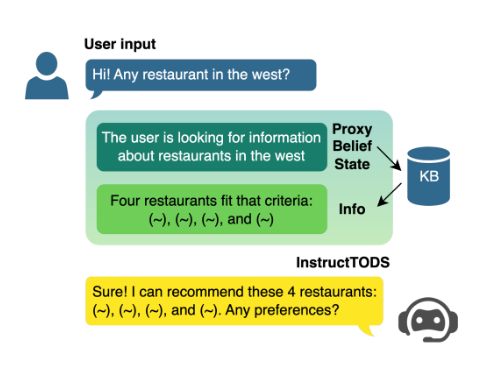
\includegraphics[width=0.5\textwidth]{InstructTODS}}
    \caption{معماری سیستم InstructTODS 
    \cite{chung2023instructtods}
    }
    \label{fig:InstructTODS}
\end{figure}


در این پژوهش، نویسندگان از مدل‌های زبانی بزرگ تنظیم شده با دستورالعمل برای ایجاد حالت باور استفاده می‌کنند که به عنوان نماینده‌ی نیت‌های کاربر عمل می‌کند و پایگاه‌های دانش را به صورت پویا در زبان طبیعی جستجو می‌کند. سپس اطلاعات بازیابی شده برای تولید پاسخ استفاده می‌شود. بر خلاف سیستم‌های سنتی وظیفه‌گرا که به مولفه‌های مجزا مانند طبقه‌بندی هدف و ردیابی وضعیت باور نیاز دارند، InstructTODS این فرآیندها را از طریق مدل‌های زبان بزرگ ادغام می‌کند و پاسخ‌ها را مستقیماً از ورودی‌های کاربر تولید می‌کند.
\newline
ارزیابی‌های جامع روی وظایف فرعی سیستم‌های گفتگو وظیفه‌گرا شامل ردیابی حالت گفتگو، طبقه‌بندی نیت، و تولید پاسخ نشان می‌دهد که InstructTODS عملکرد مشابهی با سیستم‌های 
کاملاً تنظیم‌شده%
\LTRfootnote{Fully fine-truned}
 دارد و حتی در شرایط صفر شات قادر است مکالمات را به طور مؤثر هدایت کند. همچنین، ارزیابی‌های انسانی نشان داده که از نظر مفید بودن، طبیعی بودن، و آموزنده بودن، InstructTODS از مدل‌های پیشرفته سیستم‌های گفتگو وظیفه‌گرا برتر است%
% Zhao-2023
\cite{madotto2021few}
.

جوانب مثبت پژوهش فوق به شرح زیر است:
\begin{itemize}
\item
قابلیت صفر شات: بدون نیاز به تنظیم دقیق یا داده‌های خاص وظیفه می‌توان از این سیستم استفاده کرد.
\item
تطبیق‌پذیری: توانایی کار با پایگاه‌های دانش متنوع بدون نیاز به مقادیر شکاف یا هستی‌شناسی‌های از پیش تعریف شده.
\item
کاهش هزینه‌های منابع: این رویکرد نسبت به سیستم‌های سنتی سیستم‌های گفتگو وظیفه‌گرا منابع کمتری نیاز دارد و کارایی را افزایش می‌دهد.
\item
گفتگوی طبیعی‌تر: بر اساس ارزیابی‌های انسانی، پاسخ‌های تولید شده طبیعی‌تر و مفیدتر هستند.
\end{itemize}

همچنین جوانب منفی این پژوهش نیز به شرح زیر است:
\begin{itemize}
\item
محدودیت‌های مدل‌های زبانی بزرگ: استفاده از مدل‌های زبانی بزرگ نیازمند منابع محاسباتی زیادی است که ممکن است در برخی موارد چالش‌برانگیز باشد.
\item
مشکلات بالقوه تعمیم: با اینکه روش صفر شات انعطاف‌پذیر است، ممکن است در وظایف خاص دامنه‌ای دچار مشکل شود.
\item
موارد شکست: در برخی از وظایف پیچیده‌تر، مدل ممکن است به درک زمینه‌ای بیشتری نیاز داشته باشد و شکست بخورد.
\end{itemize}

در %
\cite{madotto2021few}

، تمرکز بر شخصی‌سازی و نمایه‌سازی کاربر است تا سیستم‌های گفتگوی وظیفه‌محور به طور پویا بر اساس ترجیحات کاربر سازگار شوند. همچنین به چالش‌هایی مانند شروع سرد، حریم خصوصی، و امتیاز تعامل کاربر پرداخته‌‌شده است. برخلاف InstructTODS که بیشتر بر سازگاری عمومی و یادگیری صفر شات تمرکز دارد، رویکرد این تحقیق به شخصی‌سازی عمیق‌تر و تعامل کاربر با سیستم توجه ویژه‌ای دارد. استفاده از پروفایل کاربر به سیستم اجازه می‌دهد که پاسخ‌ها را با دقت بیشتری به نیازهای کاربر تنظیم کند، در حالی که InstructTODS بیشتر بر کارایی و سازگاری با پایگاه‌های دانش عمومی تکیه دارد. در حالی که هر دو سیستم به کاهش پیچیدگی در سیستم‌های گفتگو وظیفه را کمک می‌کنند، تفاوت اساسی در نحوه رسیدگی به نیازهای کاربران وجود دارد. رویکرد رساله فوق با تمرکز بر پروفایل کاربر، تجربه کاربر را بهینه می‌کند، در حالی که InstructTODS به انعطاف‌پذیری عمومی در تنظیمات مختلف توجه دارد.

\subsubsection{سیستم گفتگوی دامنه باز}
سیستم‌های گفتگوی دامنه باز برای درگیر شدن در گفتگو در مورد طیف گسترده‌ای از موضوعات بدون هدف یا هدف خاصی طراحی شده‌اند. برخلاف سیستم‌های وظیفه‌محور، که هدفشان دستیابی به یک نتیجه خاص (مانند رزرو پرواز یا ارائه پشتیبانی مشتری) است، سیستم‌های دامنه باز بر حفظ یک مکالمه طبیعی و روان تمرکز می‌کنند.


در % 
\cite{madotto2021few}
 ربات چند شات%
\LTRfootnote{Few-Shot Bot}
: یادگیری مبتنی بر پرامپت برای سیستم های گفتگو، سیستمی معرفی شده که بر مبنای یادگیری مبتنی بر پرامپت و چند شات طراحی شده است و به کمک چند نمونه مکالمه می‌تواند پاسخ‌های گفتگو محور را تولید کند. این سیستم بدون نیاز به تنظیم دقیق مدل و تنها با استفاده از پرامپت‌های محدود، قادر به مدیریت مکالمات مختلف است. این پژوهش به بررسی کاربردهای مختلف این رویکرد پرداخته و از جمله وظایف گفتگو، تولید پاسخ، پردازش مکالمات، و ایجاد پرسونا را ارزیابی کرده است. روش‌های مبتنی بر پرامپت به مدل‌های زبانی این امکان را می‌دهند که با بهره‌گیری از حداقل داده، عملکردی نزدیک به مدل‌های کاملاً آموزش‌دیده داشته باشند.
\newline
سهم اصلی این پژوهش، معرفی سیستم ربات چند شات است که از یادگیری چند شات مبتنی بر پرامپت بهره می‌برد تا به جای تنظیم دقیق و پرهزینه مدل‌های بزرگ زبانی، از چند نمونه مکالمه برای آموزش استفاده کند. این سیستم از توانایی یادگیری از طریق پرامپت‌ها بهره برده و با استفاده از مکانیزم 
انتخاب‌گر مهارت%
\LTRfootnote{Skill Selector}
، بهترین پاسخ را بر اساس تاریخچه مکالمات انتخاب می‌کند و از این طریق می‌تواند با جستجو در پایگاه‌های دانش پاسخ‌های طبیعی و مرتبط ارائه دهد.
\newline
دو چالش اصلی که در%
\cite{madotto2021few}
 به آن‌ها پرداخته شده عبارت‌اند از: 
\begin{enumerate}
\item
 هزینه بالای تنظیم و آموزش مدل‌های بزرگ زبانی: این مدل‌ها به منابع محاسباتی قابل‌توجهی نیاز دارند که باعث افزایش 
هزینه‌های عملیاتی و زمان‌بری فرایند آموزش می‌شود. این پژوهش تلاش کرده با استفاده از یادگیری چند شات مبتنی بر پرامپت، رویکردی کم‌هزینه و کارآمد ارائه دهد.
\item
نبود بنچمارک‌های رسمی برای ارزیابی روش‌های مبتنی بر پرامپت در سیستم‌های گفتگو: در این پژوهش، نویسندگان با بررسی یازده مجموعه داده مرتبط با مکالمات، یک بنچمارک رسمی برای یادگیری مبتنی بر پرامپت ارائه کرده‌اند که به ارزیابی عملکرد و مقایسه با روش‌های متداول کمک می‌کند.
\end{enumerate}

نویسندگان برای توسعه ربات چند شات از رویکردی استفاده کرده‌اند که در آن مدل‌های زبانی با نمونه‌های کوچک و بهینه‌شده هدایت می‌شوند. این سیستم از پرامپت‌های چند شات استفاده می‌کند و قادر است مکالمات متنوعی را مدیریت کرده و پاسخ‌های مناسبی ارائه دهد. از سوی دیگر، یک انتخاب‌گر مهارت به سیستم اضافه شده که بر اساس داده‌های ورودی، بهترین مهارت  مورد نیاز یک مکالمه را برای هر سوال انتخاب می‌کند. در این رویکرد، از هیچگونه تنظیم دقیق برای بهینه‌سازی مدل استفاده نمی‌شود و تنها پرامپت‌های کوتاه و ساده هدایتگر مدل هستند.

ارزیابی و نتایج پژوهش با استفاده از چندین معیار ارزیابی، از جمله تولید پاسخ‌های دقیق، پردازش پرسونا و ارزیابی‌های انسانی، نشان داده که ربات چند شات در بسیاری از موارد توانسته است به عملکردی مشابه یا بهتر از مدل‌های کاملاً تنظیم‌شده دست یابد. نتایج حاکی از آن است که این سیستم بدون نیاز به تنظیم دقیق و تنها با بهره‌گیری از پرامپت‌های چند شات، قادر به تولید پاسخ‌های طبیعی و مرتبط است که این رویکرد برای محیط‌هایی که نیاز به تنظیم دقیق و منابع زیاد ندارند، مناسب است.
\newline
از جمله مزایای اصلی این رویکرد، کاهش چشمگیر هزینه‌های محاسباتی است. به دلیل عدم نیاز به تنظیم دقیق و استفاده تنها از پرامپت‌ها، هزینه‌ها به میزان قابل‌توجهی کاهش یافته و این روش سازگاری مناسبی با وظایف مختلف مانند چت آزاد، تولید پاسخ‌های مبتنی بر دانش و پردازش اطلاعات دارد. همچنین، استفاده از انتخاب‌گر مهارت و یادگیری مبتنی بر پرامپت، باعث افزایش دقت پاسخ‌ها و تناسب آن‌ها با نیازهای کاربر می‌شود. 
\newline
از معایب این روش می‌توان به نیاز به طراحی دقیق پرامپت‌ها اشاره کرد که برای هر وظیفه نیازمند تخصص است. همچنین، در تعاملات پیچیده و شرایط خاص دامنه، این روش ممکن است دقت کمتری نسبت به مدل‌های کاملاً تنظیم‌شده داشته باشد.

پژوهش «XDAI: چارچوبی بدون تنظیم برای بهره‌برداری از مدل‌های زبانی از پیش آموزش‌دیده در تولید گفتگوی مبتنی بر دانش»%
\cite{yu2022xdai}
چارچوبی بدون نیاز به تنظیم دقیق ارائه می‌دهد که برای ایجاد سیستم‌های گفتگوی مبتنی بر دانش طراحی شده است. این سیستم از مدل‌های زبانی از پیش‌آموزش‌دیده استفاده می‌کند و تلاش می‌کند تا چالش‌های موجود در ساخت چنین سیستم‌هایی، از جمله گردآوری منابع دانش و نیاز به تنظیم مدل‌ها، را کاهش دهد. با استفاده از XDAI، توسعه‌دهندگان می‌توانند به سرعت سیستم‌های گفتگوی عمومی یا خاص دامنه ایجاد کنند. \\


مهم‌ترین نوآوری%
\cite{yu2022xdai}
 ارائه چارچوب XDAI است که شامل ویژگی‌های زیر است:
\begin{enumerate}
\item
 شروع سریع: ارائه یک سرویس گفتگوی مبتنی بر دانش که از منابع آماده برای دامنه عمومی استفاده می‌کند.
\item
 استنتاج کارآمد: استفاده از الگوهای پرسشی جدید که کیفیت دیالوگ‌ها را بدون نیاز به تنظیم دقیق مدل بهبود می‌بخشند.
\item
 استقرار سفارشی: امکان استفاده از افزونه‌های قابل تغییر برای جمع‌آوری خودکار منابع دانش خاص دامنه.
\item
 تغییرات افزایشی: ابزارهایی برای توسعه و شخصی‌سازی تدریجی سیستم فراهم می‌کند.
\end{enumerate}
در%
\cite{yu2022xdai}
 آزمایش‌های گسترده‌ای شامل ارزیابی‌های آنلاین و آزمون تورینگ انجام داده‌است و نتایج نشان می‌دهد که عملکردی رقابتی با مدل‌های پیشرفته کاملا تنظیم‌شده ارائه می‌دهد. همچنین قابلیت استفاده در دامنه‌های مختلف را با هزینه محاسباتی کمتر فراهم می‌کند.

از مزایای سیستم %
\cite{yu2022xdai}
 می توان به عدم نیاز به تنظیم دقیق و کاهش هزینه‌های محاسباتی و زمانی اشاره کرد. همچنین انعطاف‌پذیری بالا، قابلیت شخصی‌سازی و استفاده در دامنه‌های مختلف از نقاط قوت دیگر این سیستم است. علاوه بر موارد ذکرشده این سیستم ازشروع سرد پشتیبانی می کند که استفاده از قابلیت‌های شات صفر برای پاسخ‌دهی بدون نیاز به داده‌های اولیه آنرا میسر کرده است.\\

پژوهش ارایه‌شده در%
\cite{yu2022xdai}
 بر شخصی‌سازی، پروفایل‌سازی کاربران و همچنین ملاحضات حریم خصوصی تأکید دارد. در حالی که اXDAI با تمرکز بر یادگیری بدون تنظیم دقیق و تزریق دانش با پرامپت‌ها عملکردی کارآمدی ارائه می‌دهد، پژوهش رساله فوق قابلیت‌های بیشتری در زمینه تطبیق با کاربران و استفاده از پروفایل‌های کاربری برای تولید پاسخ‌های شخصی‌سازی‌شده دارد.

از معایب سیستم%
\cite{yu2022xdai}
می‌توان به کیفیت محدود پرامپت‌ها اشاره کرد. طراحی بهینه پرامپت‌ها برای وظایف پیچیده نیازمند تخصص است. همچنین عدم شخصی‌سازی عمیق را نیز می‌توان به عنوان عیب دیگری از این سیستم نام برد. در XDAI، تمرکز بیشتر بر بهره‌وری عمومی مدل‌ها و نه بر شخصی‌سازی عمیق پروفایل کاربر بوده است.


\subsection{تنظیم سریع و تکنیک های انطباق مدل}

\begin{enumerate}
\item
\textbf{تنظیم سریع برای کارایی سیستم گفتگو}

سیستم گفتگوی شخصی‌سازی‌شده با استفاده از تکنیک تنظیم سریع%
\cite{kasahara2022building}
 از روش‌های بهینه‌سازی 
بردارهای تعبیه‌شده%
\LTRfootnote{Embedding Vectors}
 برای پیش‌برد گفتگوها استفاده می‌کند. هدف اصلی این سیستم، ارائه پاسخ‌های گفتگو محوری است که هم از نظر 
پرسونا%
 \LTRfootnote{Persona}
(شخصیت از پیش تعریف شده) منسجم باشد و هم هزینه محاسباتی اندکی داشته باشد. این سیستم توانسته با به‌ حداقل رساندن تغییرات در پارامترهای اصلی مدل زبانی، کارایی مطلوبی از نظر منابع ارائه دهد.

این پژوهش به‌طور دقیق به چالش‌های 
سیستم‌های گفتگوی چند نوبتی%
\LTRfootnote{multi-turn dialogue system}
پرداخته و راه‌حل‌هایی برای بهبود شخصی‌سازی پاسخ‌ها بدون نیاز به داده‌های زیاد و قدرت محاسباتی ارائه می‌دهد. از جمله مشکلات اصلی که سیستم‌های چند نوبته با آن مواجه هستند، تناقض در پاسخ‌ها است؛ به عنوان مثال، ممکن است یک سیستم در مکالمه‌های مختلف مکان‌های متفاوتی را به عنوان محل سکونت خود اعلام کند. از طرف دیگر، سیستم‌های سنتی برای تعبیه اطلاعات شخصی در ورودی مدل، نیاز به طول ورودی زیادی دارند که کارایی را کاهش می‌دهد.
\newline
رویکرد % 
\cite{kasahara2022building}
 بر استفاده از تنظیم سریع تأکید دارد که با مسدود کردن پارامترهای مدل از پیش‌آموزش‌دیده و افزودن یک پرامپت با طول ثابت قبل از توالی ورودی، اطلاعات شخصیتی کاربر (پرسونا) را جاسازی می‌کند. 
\newline
این تکنیک از چند مولفه کلیدی تشکیل شده است:
\begin{itemize}
\item
مدل‌های زبانی از پیش‌آموزش‌دیده: استفاده از مدل‌های مبتنی بر معماری جی‌پی‌تی که از قبل قابلیت‌های گفتگوی عمومی دارند.
\item
تنظیم سریع: تنظیم تعداد کمی از بردارهای تعبیه‌شده که به خوبی می‌توانند اطلاعات شخصیت را ضبط و بهینه کنند.
\item
جاسازی اطلاعات شخصیت: این سیستم با استفاده از تعبیه‌های بهینه‌شده، اطمینان حاصل می‌کند که پاسخ‌ها با شخصیت خاص کاربر سازگار باشند.
\end{itemize}

کاساهارا و همکاران%
\cite{kasahara2022building}
 دو نوع ارزیابی خودکار و دستی را برای بررسی کیفیت سیستم ارائه داده‌اند. نتایج به زبان‌های انگلیسی و ژاپنی بررسی شده و نشان داده است که سیستم توانسته پاسخ‌هایی منسجم و طبیعی ارائه دهد. همچنین، کارایی محاسباتی سیستم در مقایسه با تنظیم دقیق کامل مدل به مراتب بالاتر است و نیاز به منابع محاسباتی کمتری دارد. مهم‌ترین معیارها در این ارزیابی‌ها شامل انسجام پاسخ‌ها بر اساس پرسونا، طبیعی بودن دیالوگ‌ها و کارایی محاسباتی بود که نتایج مطلوبی ارائه شد.

معماری روش پیشنهادی%
\cite{kasahara2022building}
 از چند لایه اصلی تشکیل شده است. ابتدا یک مدل زبانی از پیش‌آموزش‌دیده به عنوان هسته اصلی سیستم استفاده می‌شود. در این سیستم، پارامترهای مدل اصلی دست نخورده باقی می‌مانند و در عوض، یک پرامپت ثابت به ورودی مدل اضافه می‌شود که شامل اطلاعات مرتبط با شخصیت کاربر است. تنظیم سریع تنها بردارهای تعبیه‌شده مرتبط با پرامپت را بهینه می‌کند، بدون آنکه پارامترهای مدل اصلی تغییر کند. این رویکرد باعث می‌شود که سیستم بتواند با کمترین منابع، پاسخ‌هایی با توجه به شخصیت از پیش تعریف‌شده ارائه دهد.
معماری این سیستم در شکل
\ref{fig:Prompt-Tuning}
آورده شده‌است.

\begin{figure}[ht]
	\centerline{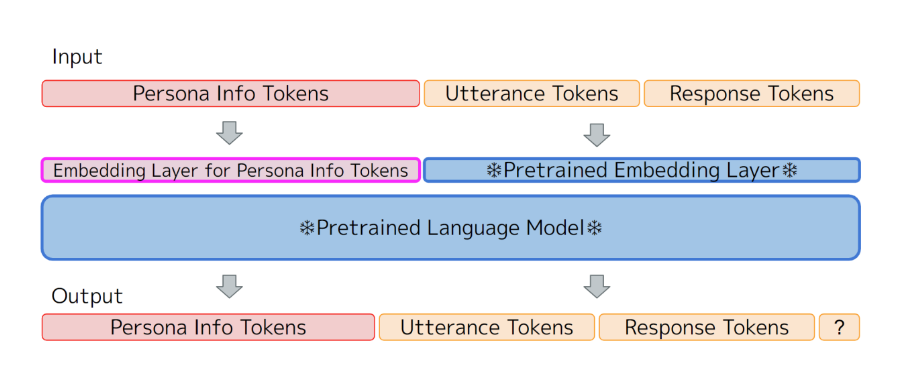
\includegraphics[width=0.8\textwidth]{8-Prompt-Tuning}}
		\caption{معماری ایجاد یک سیستم گفتگوی شخصی با تنظیم سریع 
			\cite{kasahara2022building}
	}
	\label{fig:Prompt-Tuning}
\end{figure}

مزایا و معایب سیستم به شرح زیر است.
\begin{itemize}
\item
مزایا:
\begin{itemize}
\item
کارایی محاسباتی بالا: به دلیل عدم نیاز به تغییر پارامترهای اصلی مدل، تنظیم سریع نسبت به تنظیم دقیق کامل منابع کمتری مصرف می‌کند.
\item
شخصی‌سازی با داده‌های اندک: با استفاده از داده‌های محدود (چند صد جفت گفتار-پاسخ)، سیستم می‌تواند پاسخ‌های شخصی ارائه دهد.
\item
اثربخشی بین‌المللی: سیستم در چندین زبان از جمله انگلیسی و ژاپنی عملکرد مطلوبی نشان داده‌است و از نظر زبانی قابل تطبیق است.
\item
سازگاری پرسونا: این سیستم توانسته به یکی از چالش‌های اصلی یعنی ثبات در پاسخ‌های شخصیتی به خوبی پاسخ دهد و از تضاد در مکالمات جلوگیری کند.
\end{itemize}


\item
معایب:
\begin{itemize}
\item
پیچیدگی در طراحی پرامپت: طراحی صحیح پرامپت‌ها برای هر شخصیت نیاز به تخصص دارد و اگر طراحی بهینه نباشد، ممکن است کیفیت دیالوگ کاهش یابد.
\item
محدودیت در انطباق‌پذیری: در حالی که این سیستم برای وظایف تعریف‌شده شخصیت محور عملکرد مطلوبی دارد، انعطاف‌پذیری آن در برخورد با شخصیت‌های متعدد یا وظایف پیچیده‌تر ممکن است محدود باشد.
\item
نبود مکانیزم شروع سرد: در این پژوهش به‌صراحت به مشکل شروع سرد اشاره‌ای نشده است؛ هرچند این تکنیک از طریق تنظیم سریع ممکن است برخی از مشکلات کمبود داده را کاهش دهد.
\end{itemize}
\end{itemize}
پژوهش ارائه‌شده، رویکردی کارآمد برای ایجاد سیستم گفتگوی شخصی‌سازی‌شده با استفاده از تنظیم سریع ارائه می‌دهد. این سیستم با حفظ ثبات شخصیت و مصرف حداقل منابع، توانسته است کارایی مطلوبی در چندین زبان ارائه دهد. در مقابل، تحقیقات رساله فوق به دنبال ارائه گفتگوهای هدف‌گرا و پروفایل‌سازی کاربر است که بتواند تجربه‌ای شخصی‌تر و مبتنی بر وظایف به کاربران ارائه دهد. این دو رویکرد می‌توانند در کنار یکدیگر مکمل باشند و بهبودهایی در زمینه شخصی‌سازی و انطباق‌پذیری گفتگوی هوشمند فراهم کنند.


\item
\textbf{تنظیم دقیق و رویکردهای ترکیبی}

 
دیلایت%
\LTRfootnote{DIALIGHT}
 توسعه سبک و چند زبانه و ارزیابی سیستم‌های گفتگوی وظیفه‌محور با مدل‌های زبانی بزرگ%
\cite{hu2024dialight}
، یک 
جعبه‌ابزار%
\LTRfootnote{Tool box}
 برای توسعه و ارزیابی سیستم‌های گفتگوی وظیفه‌محور چندزبانه ارائه می‌کند. این جعبه‌ابزار قابلیت مقایسه بین سیستم‌های مبتنی بر تنظیم دقیق مدل‌های زبانی از پیش آموزش دیده و سیستم‌های جدیدتر مبتنی بر مدل‌های زبانی بزرگ را دارد. دیلایت به کاربران این امکان را می‌دهد که علاوه بر ارزیابی‌های خودکار، از ارزیابی‌های انسانی دقیق در سطوح مختلف از جمله سطح گفتگو و سطح جمله نیز بهره‌مند شوند. همچنین این جعبه‌ابزار از یک معماری مبتنی بر میکروسرویس استفاده می‌کند که به مقیاس‌پذیری و کارایی بهتر کمک می‌کند 
\cite{hu2024dialight} \\
.

مشکل اصلی که در این پژوهش به آن پرداخته شده، چالش ارزیابی و توسعه‌ی کارآمد سیستم‌های گفتگوی وظیفه‌محور چندزبانه است. سیستم‌های کنونی عمدتاً بر مدل‌های زبانی از پیش آموزش دیده با تنظیم دقیق تکیه دارند که دقت بالاتری در تطبیق با وظایف خاص دارند، اما این مدل‌ها نیازمند زمان و منابع زیادی برای تنظیم هستند. از طرف دیگر، سیستم‌های مبتنی بر مدل‌های زبانی بزرگ از قابلیت تولید پاسخ‌های متنوع‌تر و طبیعی‌تر بهره‌مند هستند، اما مشکلاتی در اجرای دقیق دستورالعمل‌ها و تولید پاسخ‌های چندزبانه دارند.
\cite{hu2024dialight} \\
 دیلایت با ارائه‌ی یک جعبه‌ابزار جامع برای ارزیابی این دو رویکرد، شکاف موجود را برطرف می‌کند.

رویکرد اصلی دیلایت به شرح زیر است:
\begin{itemize}
\item
تنظیم دقیق مدل‌های مدل‌های زبانی از پیش آموزش‌دیده: دیلایت امکان تنظیم دقیق مدل‌های زبانی از پیش آموزش‌دیده برای تطبیق آن‌ها با وظایف خاص را فراهم می‌کند. این فرایند بر اساس آموزش مدل‌ها بر روی داده‌های مکالمه‌ی وظیفه‌محور انجام می‌شود.
\item
یادگیری درون‌زمینه%
\LTRfootnote{In-Context Learning}
 و بدون شات: سیستم‌های مبتنی بر مدل‌های زبان بزرگ بدون نیاز به تنظیم دقیق می‌توانند مکالمات وظیفه‌محور را در حالت‌های شات صفر و چندشات تولید کنند، اگرچه محدودیت‌هایی در تطابق دقیق با وظایف خاص دارند.
\item
پلتفرم چندزبانه: دیلایت امکان ارزیابی سیستم‌های گفتگو را در زمینه‌های تک‌زبانه، چندزبانه و حتی بین‌زبانی فراهم می‌کند و این یک قابلیت مهم برای توسعه‌ی سیستم‌های گفتگوی چندزبانه است.
\end{itemize}

ارزیابی‌ها نشان دادند که این روش منجر به دقت بالاتر و انسجام بیشتر در پاسخ‌ها می‌شود. 
اگرچه این سیستم‌ها خروجی‌های متنوعی تولید می‌کنند، اما در پیروی از دستورالعمل‌های خاص کار و ایجاد پاسخ‌های دقیق چندزبانه محدودیت‌هایی دارند. این مشکلات نشان‌دهنده نیاز به تحقیقات بیشتر در این حوزه است.

 مزایای این سیستم به شرح زیر است.
\begin{itemize}
\item
پشتیبانی از یادگیری بدون شات و درون‌زمینه: سیستم‌های مدل‌های زبانی بزرگ می‌توانند بدون نیاز به تنظیم دقیق، پاسخ‌های مورد انتظار در حالت‌های شات صفر و چندشات تولید کنند.
\item
ارزیابی چندزبانه و بین‌زبانی: دیلایت می‌تواند به‌صورت یکپارچه سیستم‌های گفتگوی وظیفه‌محور را در زبان‌های مختلف و حتی میان‌زبانی ارزیابی کند، که این یک نیاز مهم در توسعه سیستم‌های گفتگوی چندزبانه است.
\item
معماری مقیاس‌پذیر: استفاده از میکروسرویس‌ها امکان مقیاس‌پذیری بالا و کارایی بهتر را در ارزیابی‌ها فراهم می‌کند.
\item
ارزیابی جامع انسانی و خودکار: دیلایت با ترکیب ارزیابی‌های انسانی و خودکار دید جامعی از عملکرد سیستم‌ها ارائه می‌دهد.
\end{itemize}

همچنین از معایت دیلایت می توان به موارد زیر اشاره کرد.
\begin{itemize}
\item
مشکلات مدل‌های زبانی بزرگ در تطبیق با وظایف خاص: سیستم‌های مدل‌های زبانی بزرگ با چالش‌هایی در پای‌بندی دقیق به وظایف خاص و تولید پاسخ‌های منسجم مواجه هستند.
\item
مصرف منابع محاسباتی زیاد: استفاده از مدل‌های زبانی بزرگ برای سیستم‌های گفتگوی وظیفه‌محور منابع محاسباتی بالایی نیاز دارد.
\item
پیچیدگی تنظیم دقیق مدل‌های زبانی از پیش آموزش‌دیده: فرایند تنظیم دقیق مدل‌های زبانی از پیش آموزش دیده نیازمند منابع زیاد است، اما در مقایسه با مدل‌های زبانی بزرگ منجر به دقت و انسجام بیشتری در پاسخ‌ها می‌شود.
\end{itemize}

در مقایسه با روش ارایه‌شده رساله فوق، که بر شخصی‌سازی سیستم‌های گفتگو و حل مشکلات شروع سرد و حق فراموشی تمرکز دارد، دیلایت بیشتر به ارزیابی عملکرد سیستم‌های گفتگوی وظیفه گرا در زبان‌های مختلف و مقایسه بین روش‌های تنظیم دقیق مدل‌های زبانی از پیش آموزش دیده و مدل‌های زبان بزرگ پرداخته است. رساله فوق علاوه بر اینکه به یادگیری شات صفر و شخصی‌سازی مکالمات توجه دارد، به مشکلات حریم خصوصی و حق فراموشی نیز می‌پردازد که در دیلایت به‌طور خاص به آن پرداخته نشده است. \\

در %
\cite{samarinas2024simulating}
با عنوان «شبیه‌سازی گفتگوهای وظیفه‌گرا با استفاده از نمودارهای انتقال حالت و مدل‌های زبان بزرگ»، به معرفی 
سینتود%
\LTRfootnote{SynTOD}
 پرداخته است. این چارچوب نوآورانه برای تولید داده‌های مصنوعی طراحی‌شده که به توسعه و ارتقاء سیستم‌های گفتگوی وظیفه‌گرا کمک می‌کند. با استفاده از نمودارهای 
انتقال حالت%
\LTRfootnote{State Transition Graphs (STGs)}
 و مدل‌های زبانی بزرگ، سینتود مکالمات ساختاریافته‌ای را شبیه‌سازی می‌کند. مهم‌ترین ویژگی این چارچوب توانایی آن در تولید مجموعه داده‌های مصنوعی متنوع و غنی برای آموزش سیستم‌های گفتگو است که به مشکل کمبود داده‌های متنوع، که یکی از چالش‌های اصلی در آموزش مدل‌های گفتگو محور محسوب می‌شود، رسیدگی می‌کند.
در این پژوهش، سینتود به عنوان راه‌حلی برای تولید داده‌های مصنوعی معرفی شده که از جمع‌آوری داده‌های دنیای واقعی بی‌نیاز است. این چارچوب با استفاده از نمودارهای انتقال حالت به سیستم اجازه می‌دهد تا مکالمات را در قالب مسیرهای مشخص هدایت کند و سپس مدل‌های زبانی بزرگ این مسیرها را دنبال کرده و مکالمات وظیفه‌گرا تولید کنند. این مکالمات مصنوعی به بهبود عملکرد سیستم‌های گفتگویی، به ویژه در وظایف پیچیده نظیر طبقه‌بندی هدف، پر کردن شکاف و تولید پاسخ کمک می‌کنند.
\newline
یکی از چالش‌های اساسی که در طراحی سیستم‌های گفتگو وظیفه‌گرا مطرح است، کمبود داده‌های متنوع و باکیفیت برای آموزش این سیستم‌ها است. مدل‌های موجود به دلیل محدودیت‌های مرتبط با داده‌ها اغلب در انجام وظایف پیچیده مانند پاسخ‌دهی به سؤالات کاربران و دسته‌بندی مقاصد کاربران دچار مشکل هستند. روش‌های سنتی جمع‌آوری داده‌ها، مانند جمع‌سپاری، معمولاً پرهزینه و زمان‌بر هستند و نمی‌توانند حجم کافی از داده‌های لازم را برای توسعه سیستم‌های قوی فراهم کنند.
به علاوه، مدل‌های زبانی بزرگ که صرفاً برای تولید مکالمات استفاده می‌شوند، غالباً در ایجاد تنوع در مکالمات ناکام هستند و داده‌های تولید شده توسط آنها، پیچیدگی و عمق کافی برای انجام وظایف گوناگون را ندارند. سینتود با تولید مجموعه‌های داده مصنوعی از طریق ترکیب نمودارهای انتقال حالت و مدل‌های زبانی بزرگ، به این مشکل رسیدگی کرده و امکان تولید مکالمات متنوع و چندبعدی را فراهم می‌کند که در دامنه‌های مختلف وظیفه‌گرا قابل استفاده هستند.
\newline
سینتود با استفاده از نمودارهای انتقال حالت و 
پیاده‌روی‌های تصادفی%
\LTRfootnote{Random Walks}
 برای شبیه‌سازی مکالمات وظیفه‌گرا یک رویکرد جامع و ساختاریافته ارائه می‌دهد. 
مراحل این رویکرد به شرح زیر است:

\begin{itemize}
\item
نمودار انتقال حالت: در این بخش از سیستم، ساختار و جریان کلی مکالمه تعریف می‌شود. نمودار انتقال حالت نشان می‌دهد که یک کاربر از طریق مقاصد و نیازهای مختلف چگونه می‌تواند با سیستم تعامل کند. این نمودار جریان‌های مکالمه و پاسخ‌های سیستم به کاربران را در قالب حالات مختلف و گذرها به تصویر می‌کشد. نمودارهای انتقال حالت کمک می‌کنند تا مکالمات منطقی و پیش‌بینی‌پذیر طراحی شوند.
\item
پیاده‌روی‌های تصادفی: سینتود از پیاده‌روی‌های تصادفی برای پیمایش نمودارهای انتقال حالت استفاده می‌کند. این کار باعث می‌شود که سیستم بتواند مکالمات متنوع و چندگانه را تولید کند. هر بار که سیستم از یک نمودار عبور می‌کند، حالت‌های جدیدی در مکالمه به وجود می‌آیند که منجر به تولید مسیرهای متفاوت و متنوع می‌شود. این امر به سیستم امکان می‌دهد تا بتواند در شرایط مختلف، عملکردهای متفاوتی را به نمایش بگذارد.
\item
شبیه‌سازی پاسخ با مدل‌های زبان بزرگ: در مرحله نهایی، از مدل‌های زبان بزرگ تنظیم‌شده برای تولید پاسخ‌های طبیعی در مکالمات استفاده می‌شود. برخلاف روش‌های ساده که تنها به تولید یک پاسخ بر اساس یک ورودی می‌پردازند، در اینجا مدل‌های زبانی بزرگ از طریق شبیه‌سازی مکالمات در مسیرهای مختلف، پاسخ‌های ساختاریافته و مبتنی بر مکالمه تولید می‌کنند.
\end{itemize}

سینتود در دو دامنه مختلف مورد ارزیابی قرار گرفته است: کمک آشپزی و تجارت الکترونیک. در هر دو حوزه، عملکرد سینتود از طریق ارزیابی‌های خودکار و ارزیابی‌های انسانی مورد بررسی قرار گرفت. ارزیابی‌های خودکار شامل معیارهایی نظیر دقت و یادآوری بود که عملکرد سیستم را در انجام وظایف مختلف مانند طبقه‌بندی هدف و پر کردن شکاف‌ها بررسی کردند.
\newline
در کنار ارزیابی‌های خودکار، ارزیابی‌های انسانی نیز انجام شد تا کیفیت و انسجام مکالمات تولید شده توسط سیستم بررسی شود. نتایج نشان داد که سینتود قادر است مکالمات غنی‌تر و متنوع‌تری نسبت به مدل‌های ساده مبتنی بر یک ورودی ایجاد کند. به‌ویژه، مکالمات تولید شده توسط سینتود نسبت به مکالمات تک‌ورودی که توسط مدل‌های زبانی بزرگ تولید شده‌اند، بهبود قابل ملاحظه‌ای در عملکرد وظایف نشان دادند.

از مزایای سینتود می‌توان بهتولید داده‌های مصنوعی بدون نیاز به جمع‌آوری داده‌های واقعی اشاره کرد. 
یکی از بزرگ‌ترین مزیت‌های سینتود این است که نیازی به جمع‌آوری داده‌های واقعی و پرهزینه ندارد. با استفاده از مدل‌های زبان بزرگ و نمودارهای انتقال حالت، می‌توان داده‌های مصنوعی متنوع و با کیفیت بالا تولید کرد که در آموزش سیستم‌های گفتگو مورد استفاده قرار می‌گیرند.
\newline
همچنین مکالمات تولید شده توسط سینتود از نظر پیچیدگی و تنوع نسبت به مکالمات جمع‌آوری‌شده یا تولید‌شده توسط مدل‌های ساده‌تر، بسیار غنی‌تر هستند. این ویژگی به سیستم‌های گفتگو امکان می‌دهد تا در موقعیت‌های پیچیده عملکرد بهتری از خود نشان دهند.
علاوه بر این سینتود توانایی انطباق با دامنه‌های مختلف وظیفه‌محور را نشان داده است و در حوزه‌هایی نظیر تجارت الکترونیک و کمک آشپزی عملکرد موفقی داشته است.

از معایت سینتود می‌توان به وابستگی به طراحی نمودار انتقال حالت اشاره کرد. کیفیت گفتگوهای تولیدشده به میزان زیادی به طراحی دقیق نمودارهای انتقال حالت وابسته است. این به معنای آن است که برای هر دامنه، باید نمودارهای اختصاصی و متناسب طراحی شود که ممکن است نیاز به تنظیمات دستی و زمان‌بر داشته باشد.
\newline
در حالی که سینتود توانسته است در حوزه‌های محدود عملکرد موفقی از خود نشان دهد، گسترش این رویکرد به حوزه‌های متنوع‌تر و وسیع‌تر ممکن است چالش‌برانگیز باشد. به‌خصوص، مقیاس‌پذیری این رویکرد در دامنه‌های پیچیده‌تر نیاز به بررسی و آزمایش بیشتر دارد.


سینتود یک چارچوب نوآورانه است که با استفاده از نمودارهای انتقال حالت و مدل‌های زبان بزرگ، امکان تولید داده‌های مصنوعی غنی و متنوع برای آموزش سیستم‌های گفتگو را فراهم می‌کند. این رویکرد به‌ویژه در زمینه‌هایی که جمع‌آوری داده‌های واقعی دشوار است، بسیار مفید است. با این حال، شخصی‌سازی و پروفایل‌سازی کاربر در این چارچوب به‌صورت مستقیم مورد توجه قرار نگرفته است. در مقایسه، در تحقیقات این رساله، به‌طور خاص بر روی مسائل مربوط به شخصی‌سازی و مدیریت هویت گوینده تمرکز شده و تلاش می‌شود با استفاده از یادگیری چند‌شات و صفر‌شات و همچنین توسعه سیستم‌های گفتگوی وظیفه‌گرا یکی از چالش‌های اصلی در هوش مصنوعی است که هدف آن، طراحی سیستم‌هایی است که بتوانند به‌صورت دقیق و هوشمندانه به تعاملات کاربران در انجام وظایف خاص پاسخ دهند. با این حال، کمبود داده‌های متنوع و باکیفیت برای آموزش این سیستم‌ها، یکی از موانع بزرگ در بهبود عملکرد آنهاست. به همین دلیل، روش‌های جدید برای تولید داده‌های مصنوعی برای توسعه و آموزش این سیستم‌ها اهمیت ویژه‌ای پیدا کرده است.\\


سکوویچ و همکاران
\cite{sekulic2024reliable}
در پژوهش شبیه‌ساز کاربر مبتنی بر مدل‌های زبانی بزرگ قابل اعتماد برای سیستم‌های گفتگوی وظیفه‌گرا، به معرفی 
شبیه‌ساز کاربر آگاه از دامنه%
\LTRfootnote{Domain-aware user simulator}
 می‌پردازد. شبیه‌ساز کاربر آگاه از دامنه یک شبیه‌ساز مولد برای سیستم‌های گفتگوی وظیفه‌گرا است که از مدل‌های زبانی بزرگ استفاده می‌کند و با تنظیم دقیق آن‌ها بر داده‌های مکالمه‌ای خاص هر دامنه، به بهبود شبیه‌سازی کاربر می‌پردازد. هدف اصلی پژوهش، کاهش مشکلات مربوط به توهمات در شبیه‌سازی‌های کاربر و ایجاد تعاملات منسجم‌تر و مرتبط‌تر است که باعث افزایش دقت در شبیه‌سازی کاربران واقعی می‌شود. در نتیجه، شبیه‌ساز کاربر آگاه از دامنه ارزیابی و توسعه سیستم‌های گفتگو وظیفه‌گرا را به‌ویژه در تشخیص خطاها و دستیابی کاربران شبیه‌سازی‌شده به اهداف مشخص‌شده تسهیل می‌کند.
\newline
این پژوهش به مسئله عدم قابلیت اطمینان و ناسازگاری شبیه‌سازهای کاربر موجود می‌پردازد. روش‌های موجود معمولاً به سیستم‌های مبتنی بر قوانین سفت و سخت یا داده‌های حاشیه‌نویسی شده تکیه می‌کنند که منجر به تعاملات شبیه‌سازی‌شده نادرست و نامربوط می‌شوند. چالشی اصلی، توهمات شبیه‌ساز است که در آن سیستم محتوای نامرتبط یا متناقض تولید می‌کند. شبیه‌ساز کاربر آگاه از دامنه با کاهش توهمات و افزایش انسجام شبیه‌ساز با اهداف کاربر، به رفع این چالش می‌پردازد.
\newline
روش پیشنهادی شبیه‌ساز کاربر آگاه از دامنه شامل موارد زیر است:
\begin{itemize}
\item
تنظیم دقیق بر داده‌های دامنه‌محور: مدل‌های زبان بزرگ از طریق تنظیم دقیق بر روی مکالمات خاص دامنه‌ای، توانایی حفظ انسجام و مرتبط بودن مکالمات را افزایش می‌دهند.
\item
شبیه‌سازی مبتنی بر اهداف کاربر: شبیه‌ساز کاربر آگاه از دامنه با شروع از اهداف مشخص شده برای کاربر، با سیستم‌های گفتگوی وظیفه‌گرا تعامل می‌کند و دیالوگ‌های چندنوبتی ایجاد می‌کند.
\item
کاهش توهمات: تنظیم دقیق شبیه‌ساز کاربر آگاه از دامنه بر داده‌های خاص هر دامنه به کاهش توهمات کمک می‌کند و پاسخ‌های مرتبط‌تر و با دقت بیشتری را تولید می‌کند.
\item
تشخیص خطا: شبیه‌ساز کاربر آگاه از دامنه برای شناسایی خطاهای رایج در سیستم‌های گفتگوی وظیفه‌گرا طراحی شده است، که این امر باعث بهبود دقت و عملکرد سیستم می‌شود.
\end{itemize}

شبیه‌ساز کاربر آگاه از دامنه با استفاده از دو معیار معتبر در ارزیابی سیستم‌های گفتگوی وظیفه‌گرا مورد آزمایش قرار گرفته است. نتایج نشان می‌دهند که تنظیم دقیق مدل‌های زبانی بزرگ بر روی داده‌های خاص دامنه‌ای، انسجام بیشتری با اهداف کاربران فراهم می‌کند و توهمات را کاهش می‌دهد.

دستاوردهای کلیدی ارزیابی شامل موارد زیر است:
\begin{itemize}
\item
بهبود تحقق اهداف کاربر: شبیه‌ساز کاربر آگاه از دامنه منجر به تعاملات موفق‌تری شد که در آن کاربران شبیه‌سازی شده به اهداف تعیین‌شده خود رسیدند.
\item
کاهش توهمات: مدل‌های زبانی بزرگ  تنظیم شده کمتر مستعد تولید پاسخ‌های نامرتبط و نامنسجم بود.
\item
تنوع واژگانی: شبیه‌ساز کاربر آگاه از دامنه با ارائه تنوع زبانی در دیالوگ‌های شبیه‌سازی شده، اما در مقایسه با روش‌های یادگیری درون‌زمینه‌ای، کمی تنوع کمتری دارد.
\end{itemize}
از مزایای این سیستم می‌توان به انطباق ویژه دامنه اشاره کرد. تنظیم دقیق بر روی داده‌های دامنه‌محور، مکالمات منسجم‌تر و مرتبط‌تری را تولید می‌کند. همچنین تمرکز شبیه‌ساز کاربر آگاه از دامنه بر انسجام مکالمات باعث کاهش توهمات می‌شود و پاسخ‌های قابل اعتمادتر و دقیق‌تری ارائه می‌دهد.شبیه‌ساز کاربر آگاه از دامنه نیازی به دسترسی به عملکرد داخلی یا سیاست‌های سیستم ندارد، که آن را به یک راه‌حل منعطف تبدیل می‌کند. این شبیه‌ساز قادر به تشخیص خطاهای رایج در سیستم‌های گفتگوی وظیفه‌گرا است و به بهبود عملکرد کلی سیستم کمک می‌کند.
\newline
از معایب سیستم 
\cite{sekulic2024reliable}
 می توان به پیچیدگی محاسباتی اشاره کرد. تنظیم دقیق مدل‌های زبان بزرگ به قدرت محاسباتی زیادی نیاز دارد و ممکن است هزینه‌بر باشد.
همچنین تنوع واژگانی محدود از دیگر نقاط ضعف آن است. اگرچه شبیه‌ساز کاربر آگاه از دامنه تنوع زبانی را فراهم می‌کند، اما در مقایسه با روش‌های یادگیری درون‌زمینه‌ای، تنوع کمتری دارد. شبیه‌ساز کاربر آگاه از دامنه بر اهداف وظیفه‌محور متمرکز است و از نمایه‌سازی کاربر یا شخصی‌سازی استفاده نمی‌کند.

در مقایسه با روش ارایه‌شده در این رساله که بر شخصی‌سازی، نمایه‌سازی کاربر و حل مشکل شروع سرد تأکید دارد، تمرکز 
\cite{sekulic2024reliable}
 شبیه‌ساز کاربر آگاه از دامنه  بر کاهش توهمات و شبیه‌سازی وظیفه‌محور است. در حالی که هر دو از مدل‌های زبانی بزرگ استفاده می‌کنند، شبیه‌ساز کاربر آگاه از دامنه  بر تنظیم دقیق دامنه‌محور تمرکز دارد، در حالی که روش رساله فوق بر تنظیم سریع و استفاده از یادگیری چند‌شات برای افزایش انطباق سیستم بدون نیاز به تنظیم دقیق گسترده تأکید دارد.

\end{enumerate}

\subsection{پروفایل کاربری}
\subsubsection{تکنیک های پروفایل صریح و ضمنی}
پروفایل صریح به اطلاعاتی اشاره دارد که به‌صورت واضح و مستقیم از کاربران جمع‌آوری می‌شود. این اطلاعات معمولاً شامل وابستگی‌ها، علایق و نیازهای کاربر است که به‌طور مستقیم از طریق پرسشنامه‌ها، نظرسنجی‌ها یا تنظیمات حساب کاربری به‌دست می‌آید. اطلاعات به‌‌دست آمده، مستقیماً مربوط به خواسته‌ها و نظرات کاربر است لذا به آسانی قابل اندازه گیری هستند.
\newline
پروفایل ضمنی به اطلاعاتی اشاره دارد که به‌طور غیرمستقیم از رفتارها و فعالیت‌های کاربران در پلتفرم‌ها جمع‌آوری می‌شود. این اطلاعات از مرور رفتار کاربر، کلیک‌ها و تعاملات او به‌دست می‌آید. این داده‌ها از طریق رفتار کاربری مانند تاریخچه جستجو و خریدها جمع‌آوری می‌شود. 
\newline

بوکلیش و همکاران %
\cite{azzam2022model}
 ،
 یک رویکرد مبتنی بر یادگیری ماشینی برای پروفایل کاربر را با تجزیه و تحلیل داده‌های رسانه‌های اجتماعی آنلاین برای شناسایی اولویت‌ها، جزئیات جمعیت‌شناختی و رفتارهای کاربران بررسی می‌کند. ایده اولیه این پژوهش مدلی است که از تکنیک‌های رگرسیون برای استخراج پروفایل‌های کاربر بر اساس سن، جنسیت و سایر ویژگی‌ها و پیش‌بینی معیارهای تعامل، مانند تعداد لایک‌های پست، بر اساس فعالیت کاربر در پلتفرم‌های رسانه‌های اجتماعی مانند فیس‌بوک استفاده می‌کند. این مدل با تجزیه و تحلیل داده های صریح (سن، جنسیت) و ضمنی (پست ها، لایک ها، اشتراک گذاری ها) به ایجاد بینش کاربر کمک می کند.

پروفایل‌سازی کاربر که بر اساس تجزیه و تحلیل رسانه‌های اجتماعی انجام می‌شود، چالش‌هایی را در مدیریت و تحلیل مؤثر داده‌های گسترده و بدون ساختار این پلتفرم‌ها به همراه دارد. با افزایش حجم اطلاعات تولید شده توسط کاربران، پیش‌پردازش داده‌ها و شناسایی الگوهای رفتاری کاربران برای ایجاد پروفایل‌های دقیق، به‌ویژه در زمینه‌هایی مانند سیستم‌های توصیه‌گر و بازاریابی هدفمند، ضروری است. در این مدل، استفاده از تکنیک‌های رگرسیون برای تحلیل روابط میان داده‌های جمعیت‌شناختی و رفتارهای اجتماعی کاربر (مانند لایک کردن یا اشتراک‌گذاری) به منظور پیش‌بینی معیارهای تعامل و همچنین ایجاد پروفایل‌های شخصی به کار گرفته می‌شود.\\


سهم اصلی 
\cite{azzam2022model}
 توسعه یک مدل یادگیری ماشینی برای پروفایل کردن کاربران بر اساس فعالیت‌های رسانه‌های اجتماعی آن‌ها است که در درجه اول بر داده‌های فیس‌بوک تمرکز دارد. با استفاده از تجزیه و تحلیل داده های رسانه های اجتماعی، هدف نویسندگان پیش بینی تعامل و ترجیحات کاربر، پرداختن به چالش استخراج بینش ارزشمند از داده های گسترده، پویا و بدون ساختار در شبکه های اجتماعی است. این وظیفه در زمینه هایی مانند سیستم های توصیه کننده، بازاریابی هدفمند و تجزیه و تحلیل احساسات مرکزی است.
چالش در مدیریت و تجزیه و تحلیل موثر داده‌ها در دسته‌های مختلف، زیرمجموعه‌ها و تعاملات کاربر، مانند پست‌ها، لایک‌ها و اشتراک‌گذاری‌ها در مقیاس بزرگ است. با توجه به حجم و تنوع داده‌های اجتماعی، پیش پردازش و شناسایی نمایش‌های دقیق کاربر بر اساس داده‌های صریح (مانند سن، جنسیت) و داده‌های ضمنی (مانند رفتار کاربر) برای استخراج نمایه‌های دقیق و جامع کاربر حیاتی است.

رویکرد پیشنهادی شامل استفاده از یک مدل رگرسیون به عنوان یک ابزار پیش بینی است که رفتار کاربران را بر اساس سن، جنسیت و سایر عوامل جمعیت شناختی ارزیابی می کند. داده‌های فیس‌بوک، به‌ویژه تعاملات کاربر (لایک کردن، اشتراک‌گذاری، نظر دادن)، برای ایجاد یک مدل نمایه کاربر استفاده شد. این مطالعه از تجزیه و تحلیل داده‌های اکتشافی و تکنیک‌های رگرسیون استفاده می‌کند و یک رگرسیون تولید می‌کند که معیارهای تعامل مانند تعداد لایک‌هایی که ممکن است پست‌های کاربر دریافت کند را پیش‌بینی می‌کند. این مدل با استفاده از خطای 
آر-اسکورد%
\LTRfootnote{R-squared}
برای تعیین دقت و اثربخشی پیش‌بینی آن ارزیابی می‌شود.
\newcommand{\RLnum}[1]{#1} % Simply outputs the Persian numerals directly
\newcommand{\num}[1]{%
   \LR{\hspace{0pt}#1\hspace{0pt}}
}

عملکرد پیش‌بینی مدل با استفاده از معیار خطای آر-اسکورد سنجیده شده است و نتیجه نرخ خطای \num{۰.۱۹۹} به دست آمد. 
این عدد نشان می‌دهد که مدل تا حدی قابل قبول عمل کرده است، اما همچنان جای پیشرفت وجود دارد. بررسی نتایج نشان می‌دهد که استفاده از پروفایل‌های مبتنی بر رگرسیون می‌تواند بینش‌های مفیدی درباره الگوهای رفتار کاربران از طریق داده‌های موجود در فعالیت‌های رسانه‌های اجتماعی ارائه دهد. به بیان ساده‎تر، این مدل می‌تواند به ما کمک کند الگوها و رفتارهای کلی کاربران را بهتر درک کنیم.

اما در این مسیر، چالش‌هایی نیز وجود دارد. به عنوان مثال، درک دقیق احساسات کاربران یا تشخیص سطوح ظریف تعامل آن‌ها کار ساده‌ای نیست. این نوع الگوها اغلب پیچیده‌تر هستند و نیازمند رویکردهای پیشرفته‌تری برای تحلیل دقیق‌تر هستند%
\cite{azzam2022model}
. بنابراین، هرچند مدل فعلی می‌تواند نقطه شروع خوبی باشد، اما برای رسیدن به دقت بالاتر، توسعه روش‌های جدید و بهینه‌سازی بیشتر ضروری به نظر می‌رسد.


مزایای %
\cite{azzam2022model}
 به شرح زیر است.
\begin{itemize}
\item
کارایی در تولید پروفایل: این مدل می‌تواند به سرعت پروفایل‌هایی را بر اساس داده‌های اولیه جمعیت‌شناختی و رفتاری ایجاد کند و از وظایفی مانند بازاریابی هدفمند و تحلیل احساسات پشتیبانی کند.
\item
قابلیت اجرا در سراسر دامنه‌ها: پروفایل کاربری از طریق این مدل کاربردهای بالقوه ای در زمینه‌های مختلف دارد، مانند نظارت بر سلامت روان، بازاریابی شخصی و تجزیه‌وتحلیل رفتار مجرمانه.
\item
پروفایل صریح و ضمنی: این رویکرد داده‌های جمعیتی صریح را با بینش‌های مبتنی بر رفتار ضمنی ترکیب می‌کند، که اجازه می‌دهد تا نمایه کاربر دقیق‌تری داشته باشد.
\end{itemize}
از معایب این روش می توان به موارد زیر اشاره کرد.
\begin{itemize}
\item
پیچیدگی محدود: اتکای مدل به رگرسیون ساده ممکن است ظرفیت آن را برای ثبت روندهای رفتاری متفاوت، به ویژه در تطبیق داده بالا، محدود کند.
\item
وابستگی به داده‌های رسانه‌های اجتماعی: این مدل به‌شدت به دقت و دردسترس‌بودن داده‌های رسانه‌های اجتماعی متکی است، که ممکن است همیشه برای نمایه‌سازی جامع قابل اعتماد یا کافی نباشد.
\end{itemize}


در مقایسه با %
\cite{azzam2022model}
، تحقیقات پژوهش فوق بر توسعه یک سیستم گفتگوی شخصی متمرکز است که از پروفایل کاربر برای توصیه‌ها و تعاملات متناسب استفاده می‌کند. مولفه پروفایل کاربری همچنین شامل نمایه‌سازی ضمنی و صریح است، اما فراتر از داده‌های جمعیت‌شناختی ثابت است و شامل تجزیه و تحلیل احساسات پویا و روش‌های فیلتر مشارکتی، مانند فیلتر مشارکتی مبتنی بر آیتم می‌شود. علاوه بر این، سیستم فوق بر حل مشکل شروع سرد با ایجاد نمایه‌های کاربر اولیه بر اساس داده‌های تعامل محدود و ارائه یک تجربه شخصی از طریق تنظیم سریع با کمک یک مدل زبان بزرگ تأکید می‌کند.

در حالی که هر دو رویکرد از نمایه‌سازی استفاده می کنند، روش پیشنهادی رساله فوق با ادغام اصل حق فراموشی فراتر می‌رود و به کاربران اجازه می‌دهد تا درخواست حذف داده‌های خود را از سیستم کنند. این با مقررات حفظ حریم خصوصی مطابقت دارد، که به طور مستقیم در مدل پروفایل کاربری از تجزیه و تحلیل رسانه های اجتماعی به آن پرداخته نمی شود. علاوه بر این، تحقیق فوق به جای تکیه بر پیش‌بینی‌های مبتنی بر رگرسیون، از تنظیم دقیق و یادگیری چند شات برای بهبود سازگاری مدل و مدیریت تعاملات شخصی در یک محیط گفتگوی وظیفه‌محور استفاده می‌کند.

به طور خلاصه، در حالی که نمایه‌سازی کاربر از طریق تجزیه‌وتحلیل رسانه‌های اجتماعی بینش‌های ارزشمندی را در مورد نمایه سازی اولیه کاربر از داده های اجتماعی ارائه می دهد، هدف تحقیق فوق گسترش این قابلیت‌ها با شخصی‌سازی پیچیده، رعایت حریم خصوصی، و تعاملات سازگار با کاربر با استفاده از تکنیک‌های پیشرفته یادگیری‌ماشینی است.\\


نگ و همکاران %
\cite{nag2023knowledge}، 
 به بررسی چگونگی تحلیل و ایجاد پروفایل کاربران از داده‌های متنی چندزبانه که در رسانه‌های اجتماعی منتشر می‌شوند، می‌پردازد. هدف اصلی این مطالعه، توسعه مدلی برای تحلیل و پروفایل‌سازی کاربران بر اساس زبان‌ها و موضوعات مختلفی است که در این پلتفرم‌ها استفاده می‌شود. روش پیشنهادی با بهره‌گیری از تکنیک‌های مختلف پردازش زبان طبیعی و استفاده از منابع دانش‌بنیان همچون 
وردنت%
\LTRfootnote{WordNet}
، تلاش می‌کند که احساسات و موضوعات پنهان در پس متون چندزبانه را شناسایی و تحلیل کند.

مشکل اصلی در
\cite{nag2023knowledge}
، تحلیل و شناسایی احساسات و موضوعات مرتبط با متن‌های چندزبانه است. کاربران در پلتفرم‌های اجتماعی از زبان‌های مختلفی برای ابراز نظرات خود استفاده می‌کنند، که تحلیل این متن‌ها و شناسایی اطلاعات مرتبط را برای ماشین‌ها به چالش می‌کشد. چالش دیگر، دسترسی به منابع و پایگاه‌های‌داده مرتبط و آماده‌سازی آن‌ها برای استفاده در مدل یادگیری ماشین است.


رویکرد پیشنهادی شامل سه مرحله اصلی است:
\begin{enumerate}
\item
تشخیص زبان: در مرحله اول، زبان هر کلمه با استفاده از مقایسه 
یونیکد%
\LTRfootnote{UNICODE}
 و فهرستی از زبان‌های مختلف شناسایی می‌شود. سپس کل متن به زبان هدف (در این آزمایش، انگلیسی) ترجمه می‌شود.
\item
تحلیل احساسات: در این مرحله، با استفاده از مجموعه داده‌ای شامل کلمات با بار معنایی مثبت و منفی، احساسات متن شناسایی می‌شود. این مجموعه داده شامل ۴۰۰۰+ کلمه مثبت و ۴۰۰۰+ کلمه منفی از پایگاه داده 
کگل%
\LTRfootnote{Kaggle - https://www.kaggle.com/}
جمع‌آوری شده است.
\item
شناسایی موضوع: در مرحله نهایی، موضوع متن با استفاده از آرشیو روزنامه و وردنت شناسایی می‌شود. این آرشیو با استفاده از منابع آنلاین و سلسله‌مراتب واژگان وردنت ایجاد می‌شود که به شناسایی کلمات مرتبط با موضوعات مختلف تا سطح سوم کمک می‌کند.
\end{enumerate}
این مدل بر روی 200 پیام در ده زبان مختلف آزمایش شده است.
نتایج نشان داد که مدل پیشنهادی با دقت قابل قبولی می‌تواند احساسات و موضوعات متون را در زبان‌های مختلف شناسایی کند. هرچند، چالش‌هایی همچون پیچیدگی ترجمه‌های چندزبانه و نیاز به داده‌های آموزشی بیشتر برای بهبود عملکرد مدل نیز ذکر شده‌است.\\

این مدل می‌تواند احساسات و موضوعات را در چندین زبان تحلیل کند که آن را برای پروفایل‌سازی کاربران در محیط‌های چندزبانه مناسب می‌سازد.
همچنین این مدل با استفاده از وردنت و آرشیو روزنامه‌ها و استفاده از منابع دانش بنیان برای استخراج موضوعات متن، به بهبود تحلیل کمک می‌کند.

از معایت این روش نیاز باید به پردازش و پیش‌پردازش پیچیده اشاره کرد. فرآیند پیش‌پردازش داده‌ها و ترجمه متون چندزبانه نیازمند زمان و منابع است. همچنین ترجمه اتوماتیک به زبان هدف (انگلیسی) ممکن است معانی دقیق را در برخی از متون از دست بدهد که دقت تحلیل را تحت تاثیر قرار می‌دهد.

در مقایسه با پژوهش این رساله،
\cite{nag2023knowledge}
 تمرکز بیشتری بر پروفایل‌سازی بر اساس داده‌های چندزبانه دارد و از منابع خارجی همچون وردنت و داده‌های خبری برای شناسایی موضوعات استفاده می‌کند. در تحقیق این رساله، پروفایل‌سازی کاربر فراتر از اطلاعات صریح و احساسات متنی کاربران است و با استفاده از تحلیل احساسات و فیلترسازی مشارکتی، نمایه‌سازی دقیق‌تر و شخصی‌سازی شده‌ای از کاربران برای تعاملات گفتگو محور ارائه می‌شود.



\subsubsection{تحلیل احساسات و فیلتر کردن مبتنی بر آیتم}
تحلیل احساسات و فیلتر کردن مبتنی بر آیتم دو تکنیک مهم در سیستم‌های توصیه‌گر و پروفایل سازی کاربر هستند که به کمک آن‌ها می‌توان به طور مؤثری به پیش‌بینی تعاملات کاربران و ارائه پیشنهادات مناسب پرداخت. 
تحلیل احساسات فرآیندی است که به شناسایی و استخراج احساسات و نظرات کاربران از متون می‌پردازد. این متون می‌توانند شامل نظرات، نقدها، توییت‌ها و دیگر اشکال ارتباطی باشند. همچنین فیلترکردن مبتنی بر آیتم یک روش برای پیشنهاد دادن آیتم‌ها به کاربران بر اساس تعاملات قبلی آن‌ها با آیتم‌های مشابه است.


پترسون و همکاران %
\cite{peterson2021user}،
 یک رویکرد متمرکز بر افزایش روش‌های پروفایل کاربر برای بهبود توصیه‌ها در سیستم‌های توصیه‌گر ارائه می‌کند. این بر اهمیت پروفایل‌های پویا و دقیق کاربر در مقابله با اضافه بار اطلاعات تاکید می‌کند، چالشی رو به رشد زیرا پلتفرم‌های بیشتری حجم زیادی از محتوا را ارائه می‌دهند. این پژوهش دو روش کلیدی پروفایل را بررسی می‌کند: یک چارچوب پروفایل کاربری سلسله مراتبی و یک رویکرد پروفایل کاربر مبتنی بر برچسب که از نظریه بازی برای متعادل‌کردن ویژگی‌ها در نمایش پروفایل استفاده می‌کند.

سهم اصلی \cite{peterson2021user}، بررسی رویکردهای نوآورانه پروفایل کاربر در سیستم‌های توصیه‌گر برای بهبود دقت توصیه است. پروفایل کاربری برای سیستم‌های توصیه‌گر برای ایجاد توصیه های مرتبط که تجربه کاربر را غنی می‌کند و اضافه بار اطلاعات را کاهش می‌دهد بسیار مهم است. این کار در درجه اول به چالش ایجاد نمایه‌های کاربری قوی می‌پردازد که به‌طور دقیق علایق کاربر را در سطوح چندگانه منعکس می‌کند، و سیستم‌های توصیه‌گر را قادر می‌سازد تا محتوای متناسب و مرتبط را به طور کارآمد ارائه دهند.

مشکل بر روی ساختن پروفایل هایی متمرکز است که نه تنها علایق کاربر را به طور دقیق منعکس می‌کند، بلکه به صورت پویا با تغییرات رفتار کاربر تنظیم می‌شود. سیستم‌های توصیه‌گر سنتی اغلب با ایجاد پروفایل‌هایی که جزئیات و کلیات را متعادل می‌کند، مشکل دارند و بر ظرفیت آنها برای ارائه توصیه‌های مناسب تأثیر می‌گذارد. تمرکز این پژوهش بر چارچوب‌های پروفایل سلسله مراتبی و مبتنی‌بر برچسب، بینش‌هایی را برای دستیابی به این تعادل ارائه می‌دهد.

پترسون و همکاران در 
\cite{peterson2021user}
دو روش اصلی برای پروفایل کاربری را بررسی می‌کنند:
\begin{itemize}
\item
چارچوب پروفایل کاربری سلسله مراتبی: این رویکرد نشان‌دهنده علایق کاربر در سطوح مختلف جزئیات است. این یک ساختار لایه‌ای برای علایق کاربر ایجاد می‌کند و به سیستم‌های توصیه‌گر اجازه می‌دهد اولویت‌های کاربر را از دسته‌های گسترده تا موارد خاص درک کند. این چارچوب انعطاف‌پذیری را افزایش می‌دهد و سیستم را قادر می‌سازد تا توصیه‌هایی را در دسته‌های مختلف و جزئیات ارائه دهد.
\item
پروفایل کاربری مبتنی بر برچسب با استفاده از تئوری بازی: در این روش، تئوری بازی برای مدیریت مبادله بین ویژگی و عمومیت در پروفایل های کاربر استفاده می شود. برچسب‌های مرتبط با تعاملات کاربر وزن می‌شوند تا ارتباط آنها را منعکس کنند، بنابراین نمایه را اصلاح می‌کنند. تئوری بازی برای بهینه‌سازی این فرآیند استفاده می‌شود و اطمینان حاصل می‌کند که پروفایل‌ها نه خیلی وسیع و نه بیش از حد جزئی هستند و به توصیه‌های کارآمد و دقیق اجازه می‌دهند.
\end{itemize}
پترسون و همکاران
\cite{peterson2021user}
اثربخشی این روش ها را با تجزیه و تحلیل توانایی آنها در بهبود دقت توصیه ها و رضایت کاربر ارزیابی می کند. چارچوب سلسله مراتبی نشان داده شده است که انعطاف پذیری در سیستم‌های توصیه‌گر را فراهم می کند و با زمینه های مختلف توصیه سازگار می شود. در همین حال، تکنیک پروفایل‌سازی مبتنی بر برچسب دقت بهبود یافته‌ای را در تطبیق علایق کاربر با موارد موجود نشان می‌دهد. هر دو رویکرد در نهایت به یک فرآیند توصیه اصلاح‌شده کمک می‌کنند، و به طور موثر به مسئله اضافه بار اطلاعات رسیدگی می‌کنند.


از جوانب مثبت%
\cite{peterson2021user}
 باید به انعطاف‌پذیری و دقت این روش اشاره کرد. ساختار سلسله مراتبی اجازه می‌دهد تا توصیه‌هایی در سطوح مختلف دانه‌بندی ارائه شود و سازگاری با نیازهای کاربر بهبود یابد. همچنین روش پروفایل‌سازی مبتنی بر نظریه بازی تضمین می‌کند که پروفایل‌ها نه بیش از حد عمومی هستند و نه خیلی خاص، که منجر به توصیه‌های مرتبط‌تر می‌شود. هر دو رویکرد به سیستم‌های توصیه‌گر اجازه می‌دهند تا به علایق کاربر در حال تکامل پاسخ دهند و پروفایل ها را به‌روز و موثر نگه دارند.

از معایب 
\cite{peterson2021user}
 می توان به پیچیدگی پیاده‌سازی آن اشاره کرد. توسعه یک چارچوب سلسله مراتبی چند سطحی و اجرای نظریه بازی برای وزن‌دهی برچسب می‌تواند از نظر محاسباتی پیچیده باشد. همچنین پتانسیل ایجاد نویز در برچسب‌ها زیاد است. روش مبتنی بر برچسب به ارتباط دقیق برچسب متکی است و تگ‌های پر سروصدا یا نامربوط می توانند بر دقت پروفایل تأثیر بگذارند.

در مقایسه با تمرکز تحقیقاتی فعلی، که شامل پروفایل کاربری در سیستم‌های گفتگو می‌شود، رویکرد پترسون و همکاران بیشتر بر روی سیستم‌های توصیه‌گر برای مدیریت اضافه بار اطلاعات متمرکز است. در حالی که تحقیقات موجود بر شخصی‌سازی و نمایه‌سازی کاربر نیز تأکید می‌کند، تکنیک‌های اضافی مانند فیلترکردن مشارکتی و تجزیه و تحلیل احساسات را که به‌ویژه برای سیستم‌های گفتگو طراحی شده است، در خود جای داده است.

در تحقیقات سیستم گفتگو، شخصی‌سازی نه تنها از طریق نمایه‌سازی، بلکه از طریق تولید پاسخ پویا بر اساس تاریخچه تعامل کاربر و بازخورد ضمنی حاصل می‌شود که در پژوهش متمرکز بر سیستم‌های توصیه‌گر کمتر بر آن تأکید شده‌است. علاوه بر این، سیستم گفتگو حق فراموش شدن را در اولویت قرار می‌دهد و به حفظ حریم خصوصی و حفظ داده‌ها می پردازد - حوزه هایی که در این پژوهش پوشش داده نمی شوند.

به طور خلاصه، روش‌های نمایه‌سازی در 
\cite{peterson2021user}
، دقت توصیه‌ها و تجربه کاربر را با تأکید بر نمایش منافع چند سطحی و تعادل بهینه در استفاده از برچسب، افزایش می‌دهد. در مقابل، تحقیق فعلی بر ادغام پروفایل کاربر با شخصی‌سازی گفتگوی بلادرنگ تمرکز دارد و شامل یک چارچوب قوی برای حفظ حریم خصوصی داده‌ها است که آن را به یک رویکرد جامع‌تر برای سیستم‌های تعامل کاربر محور تبدیل می‌کند.

\subsubsection{تکنیک های پروفایل سازی کاربر برای افزایش حریم خصوصی}
ژنگ و همکاران %
\cite{zhang2024right}
  به بررسی و تحلیل مفهوم حق فراموشی در زمینه مدل‌های زبانی بزرگ پرداخته‌است. حق فراموشی به عنوان یکی از مفاد مهم حفاظت از داده‌های شخصی، ابتدا در قوانین حریم خصوصی اروپا%
\LTRfootnote{ General Data Protection Regulation (GDPR)}
 تعریف و شناخته‌شد و سپس با توسعه سریع مدل‌های زبانی بزرگ و کاربردهای آن‌ها در زمینه‌هایی نظیر سیستم‌های گفتگو به چالشی جدید تبدیل شد. برخلاف موتورهای جستجو که بر پایه ایندکس‌سازی و ساختارهای ساده‌تر به ذخیره و بازیابی اطلاعات می‌پردازند، مدل‌های زبانی بزرگ اطلاعات را به روش‌های پیچیده‌تر و در ساختارهای عصبی ذخیره و پردازش می‌کنند که اجرای حق فراموشی در آن‌ها نیازمند راهکارهای فنی پیشرفته است.

یکی از چالش‌های اصلی پیاده‌سازی حق فراموشی در مدل‌های زبانی بزرگ به چگونگی حذف کامل و دقیق داده‌های حساس از حافظه مدل‌ها برمی‌گردد. این امر به دلیل ساختار عمیق شبکه‌های عصبی و نحوه ذخیره‌سازی داده‌ها به صورت غیرمستقیم و پیچیده، بسیار دشوار است. به‌علاوه، به دلیل عدم وجود ساختارهای مشخص و قابل مشاهده برای ذخیره داده‌ها در مدل‌های زبانی بزرگ، فرآیند حذف داده‌ها به صورت جامع‌تر و دقیق‌تری نیاز دارد تا بتواند به سطحی از حریم خصوصی که با قوانین حریم خصوصی اروپا سازگار است، دست یابد. 

\cite{zhang2024right}
 با بررسی چالش‌های فنی حق فراموشی در مدل‌های زبانی بزرگ، چندین راه‌حل بالقوه را پیشنهاد کرده است که به ترتیب زیر خلاصه می‌شوند:
\begin{enumerate}
\item

عدم یادگیری ماشین%
\LTRfootnote{Machine Unlearning}
: در این رویکرد، تلاش می‌شود که مدل به شکلی بازآموزی شود که به‌طور خاص هیچ اثری از داده‌های حذف‌شده باقی نماند. این روش به ویژه در شرایطی که کاربر درخواست حذف کامل داده‌ها را دارد، می‌تواند مناسب باشد.
\item
ویرایش مدل%
\LTRfootnote{Model Editing}
: در این روش، پارامترهای مدل به نحوی تغییر داده می‌شوند که داده‌های حساس به‌طور خاص از بین بروند. در ویرایش مدل، هدف این است که مدل به گونه‌ای اصلاح شود که دیگر نیازی به مراجعه به داده‌های حذف شده نداشته باشد.
\item
حفاظت از حریم خصوصی تفاضلی %
\LTRfootnote{Differential Privacy}
: این روش با استفاده از تکنیک‌های آماری و داده‌کاوی، میزان دسترسی به داده‌های حساس را به‌طور قابل توجهی کاهش داده و همزمان عملکرد مدل را حفظ می‌کند. این رویکرد به عنوان راهکاری موثر برای حفاظت از داده‌های کاربر و انطباق با اصول حریم خصوصی شناخته می‌شود.
\end{enumerate}

در 
\cite{zhang2024right}
 تأثیرات استفاده از این رویکردها در عملکرد و دقت مدل‌های زبانی بزرگ ارزیابی شده است. نتایج نشان می‌دهد که ویرایش مدل و عدم یادگیری می‌تواند به کاهش چالش‌های حق فراموشی در مدل‌های زبانی بزرگ کمک کند. به‌علاوه، استفاده از حفاظت از حریم خصوصی تفاضلی به عنوان راهکاری موثر شناخته شده است که به مدل‌ها اجازه می‌دهد داده‌های کاربران را حذف کرده و در عین حال، سازگاری با قوانین حریم خصوصی را حفظ کنند.

 مزایا و محدودیت‌های پیاده‌سازی حق فراموشی در مدل‌های زبانی بزرگ به شرح زیر است.
\begin{itemize}
\item
- مزایا: اجرای حق فراموشی در مدل‌های زبانی بزرگ، مزایایی نظیر افزایش حفاظت از حریم خصوصی کاربران و انطباق بیشتر با قوانین حریم خصوصی مانند قوانین حریم خصوصی اروپا را به همراه دارد.
\item
- محدودیت‌ها: از معایب این راهکارها می‌توان به هزینه‌های محاسباتی بالا و کاهش احتمالی کارایی مدل‌ها پس از حذف داده‌ها اشاره کرد. 
\end{itemize}

حق فراموشی در عصر مدل‌های زبانی بزرگ 
\cite{zhang2024right}
، راه‌حل‌های مناسبی را برای اجرای حق فراموشی در سیستم‌های مبتنی بر مدل‌ زبانی بزرگ ارائه می‌دهد که می‌تواند به حفاظت از حریم خصوصی کاربران کمک کند. پژوهش حاضر در زمینه سیستم‌های گفتگو وظیفه‌گرا که به حذف داده‌های کاربران و حفظ حریم خصوصی توجه می‌کند، می‌تواند از این تکنیک‌ها بهره ببرد. این روش‌ها به پژوهش شما این امکان را می‌دهند که بدون کاهش کارایی سیستم، امکان حذف داده‌های حساس را فراهم کند و به اصول حریم خصوصی پایبند بماند.


در جدول%
\ref{tab:literatureReview}
مقایسه جامعی بین مقالات بررسی‌شده و روش ارایه‌شده در پژوهش حاضر آورده شده‌است.

 \renewcommand{\arraystretch}{1} % Set to 1 for normal row height
\setlength{\extrarowheight}{0pt} % No extra space

\begin{table}[ht]
    \caption{مقايسه پژوهش‌های انجام شده}
    \label{tab:literatureReview}
    \centering
    \onehalfspacing
   \begin{tabularx}{\textwidth}{|
					   >{\centering}m{3.5cm}|
                                   >{\centering}m{1cm}|
                                   >{\centering}m{0.6cm}|
                                   >{\centering}m{0.6cm}|
                                   >{\centering}m{0.6cm}|
                                   >{\centering}m{0.7cm}|
                                   >{\centering}m{0.6cm}|
                                   >{\centering}m{0.6cm}|
                                   >{\centering}m{0.6cm}|
                                   >{\centering}m{0.7cm}|
                                   >{\centering\arraybackslash}m{0.7cm}|
	} % Adjusted columns
        \hline
        	\rotatebox{0}{عنوان مقاله} & 
        	\rotatebox{90}{ سیستم گفتگوی وظیفه‌گرا } & 
        	\rotatebox{90}{شخصی‌سازی} & 
        	\rotatebox{90}{شروع سرد} & 
        	\rotatebox{90}{پروفایل کاربری} & 
        	\rotatebox{90}{استفاده از مدل زبانی} & 
        	\rotatebox{90}{تنظیم سریع} & 
        	\rotatebox{90}{تنظیم دقیق} & 
        	\rotatebox{90}{حق فراموشی} & 
       		\rotatebox{90}{یادگیری چند شات} & 
        	\rotatebox{90}{یادگیری بدون شات} \\
% In-Context learning
        \hline
	\rotatebox{0}{\cite{bocklisch2024task} 2024 Bocklisch,} & 
        	{\faCheck \quad} & 
        	{\textcolor{red}  \faTimes \quad} & 
        	{\textcolor{red}  \faTimes \quad} & 
        	{\textcolor{red}  \faTimes \quad} & 
        	{\faCheck \quad} & 
        	{\textcolor{red} \faTimes \quad} & 
        	{\textcolor{red} \faTimes \quad} & 
        	{\textcolor{red} \faTimes \quad} & 
      	 	{\faCheck \quad} & 
        	{\faCheck \quad} \\

% InstructTODS
         \hline
	\rotatebox{0}{\cite{chung2023instructtods} 2024 Chung,} & 
        	{\faCheck \quad} & 
        	{\textcolor{red}  \faTimes \quad} & 
        	{\faCheck \quad} & 
        	{\textcolor{red}  \faTimes \quad} & 
        	{\faCheck \quad} & 
        	{\textcolor{red} \faTimes \quad} & 
        	{\textcolor{red} \faTimes \quad} & 
        	{\textcolor{red} \faTimes \quad} & 
   	    	{\textcolor{red} \faTimes \quad} & 
        	{\faCheck \quad} \\

% DIALIGHT
         \hline
	\rotatebox{0}{\cite{hu2024dialight} 2024 Hu,} & 
        	{\faCheck \quad} & 
        	{\textcolor{red}  \faTimes \quad} & 
        	{\faCheck \quad} & 
        	{\textcolor{red}  \faTimes \quad} & 
        	{\faCheck \quad} & 
        	{\textcolor{red} \faTimes \quad} & 
        	{\faCheck \quad} & 
        	{\textcolor{red} \faTimes \quad} & 
    	   	{\textcolor{red} \faTimes \quad} & 
        	{\faCheck \quad} \\

% DAUS 
         \hline
	\rotatebox{0}{\cite{sekulic2024reliable} 2024 Sekuli,} & 
        	{\faCheck \quad} & 
        	{\textcolor{red}  \faTimes \quad} & 
        	{\textcolor{red}  \faTimes \quad} & 
        	{\textcolor{red}  \faTimes \quad} & 
        	{\faCheck \quad} & 
        	{\textcolor{red} \faTimes \quad} & 
        	{\faCheck \quad} & 
        	{\textcolor{red} \faTimes \quad} & 
   	    	{\textcolor{red} \faTimes \quad} & 
        	{\faCheck \quad} \\
 
% SynTOD 
         \hline
	\rotatebox{0}{\cite{samarinas2024simulating} 2024 Samarinas,} & 
        	{\faCheck \quad} & 
        	{\textcolor{red}  \faTimes \quad} & 
        	{\faCheck \quad} & 
        	{\textcolor{red}  \faTimes \quad} & 
        	{\faCheck \quad} & 
        	{\textcolor{red} \faTimes \quad} & 
        	{\faCheck \quad} & 
        	{\textcolor{red} \faTimes \quad} & 
       		{\textcolor{red} \faTimes \quad} & 
        	{\faCheck \quad} \\

% XDAI
         \hline
	\rotatebox{0}{\cite{yu2022xdai} 2022 Yu,} & 
        	{\faCheck \quad} & 
		{\textcolor{red}  \faTimes \quad} & 
        	{\faCheck \quad} &         	
        	{\textcolor{red}  \faTimes \quad} & 
        	{\faCheck \quad} & 
        	{\textcolor{red}  \faTimes \quad} & 
        	{\textcolor{red}  \faTimes \quad} & 
        	{\textcolor{red} \faTimes \quad} & 
       			{\textcolor{red}  \faTimes \quad} & 
        	{\faCheck \quad} \\

% Prompt-Tuning 
         \hline
	\rotatebox{0}{\cite{kasahara2022building} 2022 Kasahara,} & 
        	{\textcolor{red}  \faTimes \quad} & 
        	{\faCheck \quad} & 
        	{\textcolor{red}  \faTimes \quad} & 
        	{\faCheck \quad} & 
        	{\faCheck \quad} & 
        	{\faCheck \quad} & 
        	{\textcolor{red}  \faTimes \quad} & 
        	{\textcolor{red} \faTimes \quad} & 
       		{\faCheck \quad} & 
        	{\textcolor{red}  \faTimes \quad} \\
        
% Few-Shot Bot
         \hline
	\rotatebox{0}{\cite{madotto2021few} 2021 Madotto,} & 
        	{\textcolor{red}  \faTimes \quad} & 
        	{\faCheck \quad} & 
        	{\faCheck \quad} & 
        	{\textcolor{red}  \faTimes \quad} & 
        	{\faCheck \quad} & 
        	{\faCheck \quad} & 
        	{\textcolor{red}  \faTimes \quad} & 
        	{\textcolor{red} \faTimes \quad} & 
       		{\faCheck \quad} & 
        	{\textcolor{red}  \faTimes \quad} \\
        
% RTBF
         \hline
	\rotatebox{0}{\cite{zhang2024right} 2024 Zhang,} & 
        	{\textcolor{red}  \faTimes \quad} & 
        	{\faCheck \quad} & 
        	{\faCheck \quad} & 
        	{\faCheck \quad} & 
        	{\textcolor{red}  \faTimes \quad} & 
        	{\textcolor{red}  \faTimes \quad} & 
        	{\textcolor{red}  \faTimes \quad} & 
        	{\textcolor{red} \faTimes \quad} & 
       		{\textcolor{red}  \faTimes \quad} & 
        	{\textcolor{red}  \faTimes \quad} \\
        
% User Profiling Multilingual Texts
         \hline
	\rotatebox{0}{\cite{nag2023knowledge} 2023 Nag,} & 
        	{\textcolor{red}  \faTimes \quad} & 
        	{\faCheck \quad} & 
        	{\textcolor{red}  \faTimes \quad} & 
        	{\faCheck \quad} & 
        	{\textcolor{red}  \faTimes \quad} & 
        	{\textcolor{red}  \faTimes \quad} & 
        	{\textcolor{red}  \faTimes \quad} & 
        	{\textcolor{red} \faTimes \quad} & 
       		{\textcolor{red}  \faTimes \quad} & 
        	{\textcolor{red}  \faTimes \quad} \\
        
% User Profiling Recommender
         \hline
	\rotatebox{0}{\cite{peterson2021user} 2021 Peterson,} & 
        	{\textcolor{red}  \faTimes \quad} & 
        	{\faCheck \quad} & 
        	{\textcolor{red}  \faTimes \quad} & 
        	{\faCheck \quad} & 
        	{\textcolor{red}  \faTimes \quad} & 
        	{\textcolor{red}  \faTimes \quad} & 
        	{\textcolor{red}  \faTimes \quad} & 
        	{\textcolor{red} \faTimes \quad} & 
	       	{\textcolor{red}  \faTimes \quad} & 
        	{\textcolor{red}  \faTimes \quad} \\
        
% Current thesis
         \hline
	\rotatebox{0}{تحقیق فوق} & 
        	{\faCheck \quad} & 
        	{\faCheck \quad} & 
        	{\faCheck \quad} & 
        	{\faCheck \quad} & 
        	{\faCheck \quad} & 
        	{\faCheck \quad} & 
        	{\faCheck \quad} & 
        	{\faCheck \quad} & 
       		{\faCheck \quad} & 
        	{\textcolor{red}  \faTimes \quad} \\
        \hline
    \end{tabularx}
\end{table}
   


\section{جمع بندی}
در این فصل، تلاش شد تا مروری جامع بر مفاهیم، پژوهش‌ها، و تکنیک‌های مرتبط با موضوع رساله فوق ارائه شود. ابتدا، در بخش سیستم‌های گفتگو، بررسی‌ها نشان دادند که سیستم‌های گفتگوی وظیفه‌گرا به دلیل ساختار هدف‌محور خود، کارآمدتر و دقیق‌تر عمل می‌کنند و بیشتر مناسب کاربردهای خاص مانند سیستم‌های رزرواسیون و سیستم‌های پیشنهاددهنده هستند. 
از سوی دیگر، سیستم‌های گفتگوی دامنه‌باز به دلیل انعطاف‌پذیری در موضوعات گسترده، مناسب تعاملات آزادتر با کاربران می‌باشند، اما همچنان در مدیریت انسجام و دقت چالش‌هایی دارند.
\newline

در بخش تنظیم سریع، روش‌های جدیدی مانند یادگیری چند شات و استفاده از پرامپت‌های هوشمند معرفی شدند که بدون نیاز به تنظیم دقیق گسترده، توانسته‌اند عملکرد سیستم‌ها را در شرایط محدود داده ارتقاء دهند. این تکنیک‌ها، علاوه بر کاهش هزینه‌های محاسباتی، امکان بهره‌برداری از مدل‌های زبانی بزرگ را برای توسعه‌دهندگان با منابع محدود فراهم می‌کنند.\\
در حوزه پروفایل‌سازی کاربر، سه دسته اصلی از تکنیک‌ها تحلیل شدند:\\
پروفایل صریح و ضمنی: ترکیب داده‌های صریح (مانند سن یا علایق شخصی) و داده‌های ضمنی (مانند رفتار کاربران) به‌عنوان یک راهکار جامع برای درک ترجیحات کاربران پیشنهاد شد.  \\
تحلیل احساسات و فیلتر کردن مبتنی بر آیتم: این روش‌ها نشان دادند که تحلیل الگوهای رفتاری و احساسی کاربران می‌تواند به توصیه‌های دقیق‌تر و شخصی‌تر منجر شود.  \\
تکنیک‌های پروفایل‌سازی با تمرکز بر حریم خصوصی: به دلیل اهمیت روزافزون حریم خصوصی، روش‌هایی که کاربران را قادر به مدیریت داده‌های شخصی خود کنند، به‌عنوان راهکاری اساسی مورد توجه قرار گرفتند.

این فصل علاوه بر مرور پژوهش‌های پیشین، شکاف‌های موجود را نیز شناسایی کرد. برای مثال، چالش‌هایی مانند عدم انسجام در گفتگوی دامنه‌باز، هزینه‌های بالای تنظیم دقیق مدل‌ها، و عدم رعایت کامل حریم خصوصی در برخی تکنیک‌های پروفایل‌سازی، فرصت‌های تحقیقاتی جدیدی را برجسته می‌کنند.
\newline
با تحلیل جامع این پژوهش‌ها، روشن شد که برای توسعه سیستم‌های گفتگو مدرن و کارآمد، نیاز به ترکیبی از تکنیک‌های بهینه‌سازی (مانند تنظیم سریع)، بهره‌گیری از مدل‌های زبانی بزرگ، و تأکید بر حریم خصوصی کاربران وجود دارد. این فصل نه‌تنها بستری علمی برای ادامه تحقیق فراهم کرد، بلکه ابزارهایی را برای طراحی نوآوری‌های عملی در حوزه سیستم‌های گفتگو و پروفایل‌سازی کاربر ارائه داد.		% فصول دوم: مروری بر مطالعات انجام شده
% !TeX root=../main.tex
\chapter{روش پیشنهادی}
%\thispagestyle{empty} 
\section{مقدمه} 
در این فصل، روش پیشنهادی مورد استفاده برای توسعه و ارزیابی سیستم گفتگوی وظیفه‌گرا با رویکرد شخصی‌سازی مورد بررسی قرار می‌گیرد. این روش شامل طراحی معماری سیستم با تمرکز بر حل چالش‌های اساسی نظیر مشکل شروع سرد، شخصی‌سازی مبتنی بر نمایه کاربر، بهره‌گیری از مدل‌های زبانی بزرگ، و تضمین حق فراموشی است. 
همچنین به مراحل پیش‌پردازش داده‌ها، استفاده از تکنیک‌های تنظیم سریع و استخراج موجودیت‌های کلیدی از ورودی کاربران پرداخته می‌شود. در نهایت، مکانیزم‌های جمع‌آوری بازخورد و ارزیابی عملکرد سیستم توضیح داده خواهند شد تا نقش آن‌ها در بهبود پویای سیستم مشخص شود.

نام روش پیشنهادی فوق MindMeld است. MindMeld در واقع ادغام هوشیارانه ذهن و ماشین برای گفتگوهای شخصی‌سازی‌شده است.


ادغام هوشیارانه در واقع بیانگر ترکیب دقیق و هدفمند داده‌ها و الگوریتم‌هاست. ذهن و ماشین نشان‌دهنده تعامل بین کاربر (ذهن) و سیستم هوش مصنوعی (ماشین) است که در قلب رویکرد فوق قرار دارد. همچنین گفتگوهای شخصی‌سازی‌شده به هدف اصلی که پاسخ های سفارشی‌شده و منطبق با نیازهای کاربر است.

\section{جمع آوری و آماده سازی داده ها}
\label{chap:dataset}
این بخش به فرآیند آماده‌سازی داده‌ها برای توسعه سیستم گفتگوی وظیفه‌محور را توضیح می‌دهد. هدف این است که داده‌های خام از منابع مختلف، از جمله مجموعه‌داده 
مووی لنز%
\LTRfootnote{MovieLens}
، به داده‌های گفتگو‌محور تبدیل شوند که مناسب برای انجام تنظیم سریع یا یادگیری درون‌متنی%
\LTRfootnote{In-Context Learning}
 هستند.
\begin{enumerate}
\item
انتخاب و بررسی مجموعه‌داده مووی لنز\\
برای تحلیل اولیه و ایجاد مجموعه‌داده مکالمه‌محور، از 
\href{https://www.kaggle.com/datasets/garymk/movielens-25m-dataset}{مجموعه داده مووی لنز 25 میلیون}
 استفاده شده است. این مجموعه داده به طور گسترده در حوزه‌های مختلف از جمله سیستم‌های توصیه‌گر و فیلتر مشارکتی استفاده می‌شود. منبع این مجموعه داده سایت 
\href{https://www.kaggle.com}{کگل}
 است که حاوی بیش از 25 میلیون رتبه‌بندی، 1 میلیون برنامه برچسب و ابرداده برای 62000 فیلم است. همچنین این مجموعه داده بیش از 20 میلیون رتبه بندی فیلم و برچسب گذاری‌های کاربران است که از سال 1995 جمع آوری کرده است. \\


ویژگی‌های کلیدی این مجموعه داده به شرح زیر است.
\begin{itemize}
\item
امتیازات کاربران: داده‌های صریح شامل رتبه‌بندی کاربران برای فیلم‌ها (1 تا 5 ستاره).
\item
تگ‌ها: عبارات یا کلمات کلیدی مرتبط با فیلم که توسط کاربران اعمال می‌شوند.
\item
ژانرها: دسته‌بندی‌های فیلم، از جمله ژانرهای اکشن، کمدی، درام و غیره.
\item
اطلاعات زمانی: مهر زمانی مربوط به تعاملات کاربران با فیلم‌ها.
\end{itemize}

در این پژوهش، از دیتاست مووی لنز به عنوان یک مثال کاربردی استفاده شده است. همانطور که ذکر شد، این دیتاست شامل اطلاعات مربوط به علایق کاربران در حوزه فیلم‌ها و امتیازدهی به آن‌ها است. با این حال، روش پیشنهادی این پژوهش تنها محدود به این حوزه نیست و می‌تواند برای دیتاست‌های دیگر در حوزه‌های مختلف مانند موسیقی، کتاب، محصولات خرید آنلاین، یا حتی خدمات آموزشی تطبیق داده شود. این انعطاف‌پذیری به دلیل طراحی عمومی الگوریتم‌ها و عدم وابستگی به ویژگی‌های خاص دیتاست است.
 
جزییات روش پیشنهادی که به طور کامل در بخش%
\ref{sec:architecture}
 بیان خواهدشد شامل مراحلی است که مستقل از نوع داده‌ها عمل می‌کنند.

به عنوان مثال، در حوزه فیلم‌ها، داده‌های ورودی شامل امتیازهای کاربران به فیلم‌ها و ژانرهای مورد علاقه آن‌ها است. اما این ورودی‌ها می‌توانند به راحتی با داده‌های دیگری مانند امتیازهای کاربران به آهنگ‌ها یا کتاب‌ها جایگزین شوند. در ادامه، با استفاده از دیتاست مووی لنز، نحوه عملکرد این روش را در قالب یک مثال کاربردی شرح می‌دهیم." 

\item
ترکیب و یکپارچه‌سازی مجموعه‌داده
 
برای ایجاد یک مجموعه داده منسجم و مناسب سیستم گفتگو نیاز به داده‌هایی داریم که دارای ماهیت مکالمه‌محور باشند یا به بیان دیگر این داده‌ها باید به صورت جفت مقدارهای پرسه و پاسخ باشند تا بتوان مدل زبانی خود را با استفاده از این داده ها آموزش داد.

در وهله اول جهت ایجاد یک مجموعه داده متشکل از فیلم ها، نظرات و امتیازات کاربران و غیره به صورت یکجا، فایل‌های امتیازات کاربران، تگ‌های آنها که به فیلم‌های مختلف داده‌اند را بر اساس ستون‌های مشترک مانند آیدی فیلم و آیدی کاربران ادغام کرده و یک مجموعه داده شامل 126 هزار کورد ایجاد نمودیم.

خروجی نهایی این مجموعه داده شامل ستون های زیر است:
\begin{itemize}
\item
آیدی کاربر: شناسه یکتای هر کاربر.
\item
آیدی فیلم: شناسه یکتای هر فیلم.
\item
رتبه‌بندی: امتیاز داده‌شده توسط کاربر.
\item
تگ‌ها: برچسب‌های کاربران برای هر فیلم.
\item
ژانرها: دسته‌بندی‌های فیلم.
\end{itemize}

% جدول نمونه برای فیلدهای موجود در مجموعه داده movieRatingTag
\begin{table}[ht]
    \centering
    \caption{نمونه‌ای از داده‌های یکپارچه شده از مجموعه داده مووی لنز}
    \label{tab:movielens-sample}
    \renewcommand{\arraystretch}{1} % Adjust row height
    \begin{tabularx}{\textwidth}{|>
{\centering\arraybackslash}p{0.1\textwidth}|>
{\centering\arraybackslash}p{0.1\textwidth}|>
{\centering\arraybackslash}p{0.1\textwidth}|>
{\centering\arraybackslash}X|>
{\centering\arraybackslash}X|>
{\centering\arraybackslash}X|}
        \hline
        \textbf{userId} &
        \textbf{movieId} &
        \textbf{rating} &
        \textbf{title} &
        \textbf{genres} &  
        \textbf{tags} \\ 
        \hline
        1629 & 2 & 5.3 & Jumanji (1995) & Adventure, Fantasy & time travel \\ 
        \hline
    \end{tabularx}
\end{table}

\item
ایجاد مجموعه داده پیام‌های مکالمه‌محور:

برای آماده‌سازی مجموعه داده به فرم پرسش و پاسخ‌های گفتگو‌محور مراحل زیر انجام شد:
\begin{itemize}
\item
محاسبه شباهت کسینوسی:
\begin{itemize}
\item
تگ‌های فیلم‌ها به صورت ماتریس برداری با استفاده از CountVectorizer تبدیل شدند.
\item
شباهت کسینوسی بین بردارهای تگ محاسبه شد تا فیلم‌های مشابه شناسایی شوند.
\item
فیلم‌هایی با شباهت بالای 90٪ به عنوان موارد پیشنهادی برای همان فیلم در نظر گرفته شدند.
\end{itemize}

\item
فرمت‌دهی داده‌ها به صورت مکالمه‌ای:

از داده‌های شناسایی‌شده، ساختارهایی با پرسش و پاسخ ایجاد شد.\\
نمونه پرسش:
\begin{quote}
\begin{LTR}
Recommend movies similar to Harry Potter and the Philosopher's Stone
\end{LTR}
\end{quote}
نمونه پاسخ:
\begin{quote}
\begin{LTR}
"Harry Potter and the Chamber of Secrets" for its Hogwarts sequel, "The Lord of the Rings: The Fellowship of the Ring" for its fantasy adventure and "Percy Jackson The Olympians: The Lightning Thief" for its mythological adventure
\end{LTR}
\end{quote}
\end{itemize}

\item
محاسبه شباهت کسینوسی:
برای شناسایی شباهت بین فیلم‌ها و ایجاد جفت‌های پرسش و پاسخ مناسب، از شباهت کسینوسی استفاده شد. رابطه شباهت کسینوسی برای دو بردار متنی A و B به صورت رابطه ی %
\ref{eq:cosineSimilarity}
 تعریف می‌شود:

 
\begin{equation}
\label{eq:cosineSimilarity}
\text{شباهت کسینوسی} = \frac{\sum_{i=1}^{n} A_i \cdot B_i}{\sqrt{\sum_{i=1}^{n} A_i^2} \cdot \sqrt{\sum_{i=1}^{n} B_i^2}}
\end{equation}


که در آن مقادیر Ai​ و Bi​ مقدار ویژگی i در بردارهای A و B هستند. همچنین مقدار n برابر با تعداد ویژگی‌ها (کلمات کلیدی یا تگ‌های فیلم‌ها در اینجا) هستند.

این رابطه تضمین می‌کند که شباهت بین دو بردار بر اساس جهت آن‌ها و نه اندازه‌شان محاسبه شود. شباهت کسینوسی معمولاً برای داده‌های متنی و برداری در تحلیل‌های پردازش زبان طبیعی و مدل‌های توصیه‌گر به کار می‌رود.

روش پیاده‌سازی این رابطه به صورت فوق است:
\begin{itemize}
\item
تبدیل تگ‌ها به بردارها: با استفاده از تکنیک CountVectorizer، تگ‌های متنی مربوط به فیلم‌ها به بردارهای عددی تبدیل شدند. این تکنیک بسته کلمات%
\LTRfootnote{Bag of Words (BoW)}
 برای نمایه‌سازی متنی استفاده می‌شود.
\item
محاسبه شباهت: شباهت کسینوسی بین بردارهای مربوط به فیلم‌ها محاسبه شد. همانطور که بیان شد، فیلم‌هایی که شباهت آن‌ها بیش از 90٪ بود، به عنوان فیلم‌های مشابه در نظر گرفته شدند.
\end{itemize}

جهانگیر و همکاران%
\cite{singh2020movie}
 با استفاده از تکنیک فوق، الگوریتم‌هایی توسعه داده شده‌اند که از داده‌های مشابه مووی لنز برای شناسایی فیلم‌های مشابه استفاده می‌کنند. برای مثال، با بهینه‌سازی عبارات کلیدی و اضافه کردن وزن به ژانرها، دقت مدل‌ها افزایش یافته است.


\item
گسترش تنوع پرسش و پاسخ:

با استفاده از فیلم مرجع و فیلم هایی که شباهت کسینوسی بالایی نسبت به فیلم فوق داشته اند، مجموعه ای از فیلم ها به همراه فیلم های مشابه با آن ها را در دسترس خواهیم داشت که می تواند در ادامه ایجاد مجموعه داده مکالمه‌محور کمک کند.\\
برای شباهت بیشتر داده‌ها به گفتگوهای روزمره، 50 قالب مختلف برای پرسش و 50 قالب برای پاسخ طراحی شد.


به عنوان مثال فیلم Hard Die را در نظر بگیرید، یک نمونه پرسه به فرم زیرخواهد بود:
\begin{quote}
\begin{LTR}
Looking for hidden gems like 'Die Hard 1988' in the action genre
\end{LTR}
\end{quote}

برای فیلم های با ژانرهای مختلف یکی از ژانرها به تصادف برای ایجاد مجموعه داده استفاده می‌شود.
همچنین یک نمونه پاسخ کاندید به صورت زیر خواهد بود:
\begin{quote}
\begin{LTR}
Finding more action films similar to ‘Die Hard 1988'. How about: Hellboy 2004
\end{LTR}
\end{quote}


\item
ایجاد مجموعه‌داده نهایی: 

ساختار مجموعه‌داده نهایی به سبک زیرخواهد بود
\begin{itemize}
\item
ورودی: شامل سوالات کاربران در قالب طبیعی
\item
خروجی: لیست فیلم‌های پیشنهادی
\item
نام فیلم: فیلم ذکر‌شده در سوال
\item
سال: سال انتشار فیلم
\item
ژانر: ژانرهای فیلم.

\end{itemize}

با این روش، مجموعه‌داده‌ای شامل 210 هزار ردیف مکالمه‌ای ایجاد شد که برای مراحل بعدی در توسعه سیستم گفتگوی وظیفه‌محور مورد استفاده قرار گرفت.


\end{enumerate}

\section{معماری سیستم}
\label{sec:architecture}
\subsection{مراحل تولید پاسخ}

این معماری برای تقویت تعامل کاربر با سیستم گفتگو وظیفه‌گرا و با  توجه به چالش‌های کلیدی مانند مسائل شروع سرد، شخصی‌سازی، استفاده از مدل های بازی تنظیم شده و رعایت حق فراموشی طراحی شده‌است. هر ماژول و اجزای آن برای بهبود سازگاری سیستم، رضایت کاربر و عملکرد خاص دامنه مورد نظر طراحی شده‌اند. در ادامه کلیّت معماری پیاده‌سازی‌شده توضیح داده‌شده و در بخش‌های آتی، هر قسمت به صورت مجزا و مفصل تر مورد بحث قرار خواهد گرفت.

جهت سهولت درک توضیحات شکل%
\ref{fig:architecture}
شماره گذاری در قسمت های مختلف آن انجام شده است که در هنگام توضیح هر قسمت، شماره آن نیز رو به روی آن آورده شده است.


\begin{figure}[ht]
	\centerline{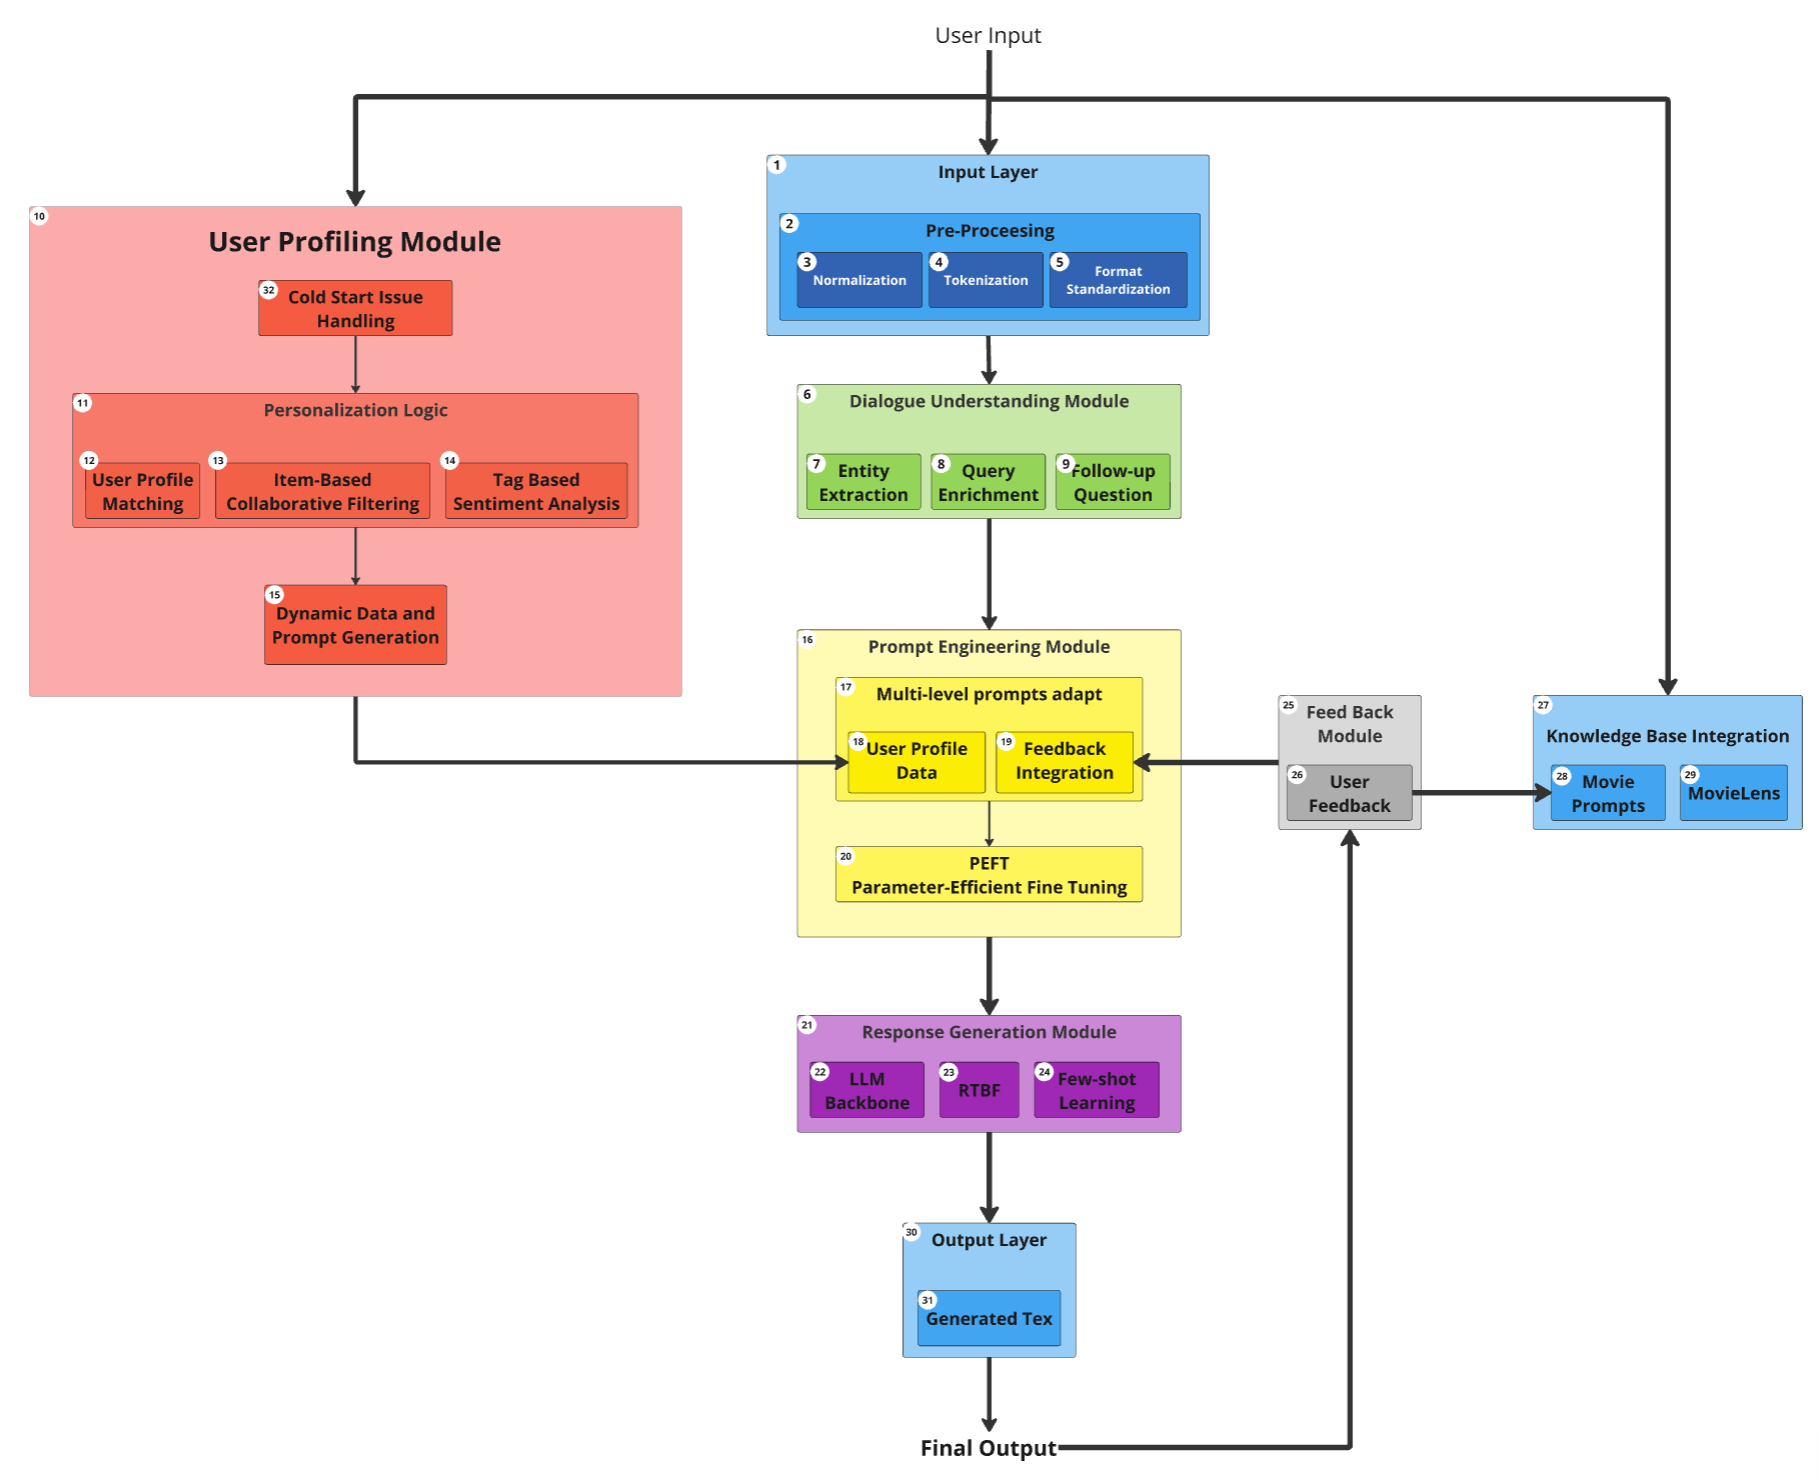
\includegraphics[width=1.0\textwidth]{architecture}}
	\caption{معماری سیستم}
	\label{fig:architecture}
\end{figure}


\begin{enumerate}
\item
 لایه ورودی
\begin{itemize}
\item
ورودی کاربر(بخش 1): این ماژول نقطه شروع دسترسی کاربر جهت پرسش سوال خود است. در این سیستم گفتگو، پرسه های مبتنی بر متن از کاربر پذیرفته می‌شود.
\item
پیش پردازش (بخش 2):
در مرحله پیش‌پردازش، داده‌های خام تمیز شده و ویژگی‌های ناقص یا نویزی حذف می‌شوند. اولین مرحله از پیش‌پردازش پرسه کاربر، 
عادی سازی%
\LTRfootnote{Normalization}
  (بخش 3) است. در این مرحله سیستم قالب متن ورودی به عنوان مثال، حروف کوچک و علامت‌گذاری را استاندارد می کند.
\item
توکن‌بندی کردن%
\LTRfootnote{Tokenization}
 (بخش 4) :متن به واحدهای قابل مدیریت (کلمات یا عبارات) شکسته می‌شود.
\item
استاندارد‌سازی فرمت%
\LTRfootnote{format standardization}
 (بخش 5) که سازگاری با ماژول‌های پردازش مراحل بعدی را تضمین می‌کند.
\end{itemize}

فرآیندهای مرحله پیش‌پردازش به طور کلی مستقل از حوزه کاربرد است و می‌تواند برای هر نوع داده‌ای اعمال شود. به عنوان مثال، در دیتاست مووی لنز، این شامل حذف رکوردهای ناقص امتیازدهی کاربران به فیلم‌ها می‌شود. اما در یک دیتاست مربوط به خرید آنلاین، این مرحله می‌تواند شامل حذف محصولاتی باشد که توضیحات ناقص دارند.
\item
 ماژول درک گفتگو (بخش 6)
\begin{itemize}
\item
استخراج موجودیت%
\LTRfootnote{Entity Extraction}
 (بخش 7) : موجودیت‌های کلیدی مانند نام فیلم و ژانرها را در پرسه کاربر را شناسایی می‌کند. اما این رویکرد به هیچ وجه محدود به فیلم‌ها نیست و می‌تواند برای استخراج ویژگی‌های دیگری مانند قیمت، برند، یا رنگ محصولات در دیتاست‌های خرید آنلاین استفاده شود.
\item
تولید‌کننده سوال بعدی%
\LTRfootnote{Follow-up question}
 (بخش 9) : برای روشن‌کردن ورودی‌های مبهم یا ناقص کاربر، درخواست‌های بعدی ایجاد می کند.
\item
غنی‌سازی پرس‌وجو%
\LTRfootnote{Query Enrichment}
 (بخش 8) : داده‌های ورودی را به صورت پویا تنظیم و اصلاح می‌کند تا درک و زمینه سیستم را بهبود بخشد. به عنوان مثال به مدل زبانی پرسه کامل به همراه فراداده هایی چون ژانر موردنظر کاربر و فیلم مورد بحث را به همراه پرسه اصلی کاربر به ورودی مدل جهت انجام عملیات تنظیم سریع بعدی ارسال می‌کند.
\end{itemize}

\item
 ماژول پروفایل کاربری (بخش 10)
\begin{itemize}
\item
رسیدگی به مشکل شروع سرد (بخش 32):\\
 زمانی که حداقل داده های کاربر در دسترس نباشد، ماژول از یک تا پنج ژانرهای مورد علاقه کاربر را از وی دریافت می‌کند و علاوه بر آن با به کارگیری فیلترمشارکتی مبتنی بر آیتم،  ترجیحات کاربر را استنتاج و استفاده می‌کند.
\item
منطق شخصی سازی (بخش 11):
\begin{itemize}
\item
تطابق نمایه کاربر (بخش 12): از داده‌های موجود کاربر، مانند امتیازات وی، تگ ها یا ژانرهای مورد علاقه (مانند استفاده از مجموعه داده مووی‌لنز) استفاده می‌کند.
\item
تحلیل احساسات مبتنی بر برچسب (بخش 14): لحن و اولویت درخواست کاربر را بر اساس داده های برچسب‌گذاری‌شده تجزیه‌وتحلیل می‌کند و آیتم‌هایی که وی به آنها تگ‌هایی با لحن مثبت و خوب داده است را استخراج می‌کند.
\item
استفاده از فیلتر مشارکتی مبتنی‌بر آیتم جهت استخراج ژانرها و فیلم‌هایی که کاربر احتمالا به آنها علاقه دارند (بخش 13).
\end{itemize}

\item
تولید داده‌های پویا و تولید پرامپت (بخش 15): رفتار سیستم را در زمان واقعی با استفاده از داده‌های نمایه کاربر تطبیق و شخصی می‌کند و یک پرسه شخصی‌سازی‌شده را به مدل ارسال می‌کند.
\end{itemize}


\item
ماژول مهندسی پرامپت (بخش 16)
\begin{itemize}
\item
تنظیم سریع: 
تنظیم دقیق پارامترهای کارآمد%
\LTRfootnote{Parameter Efficient Fine Tuning(PEFT)}
 (بخش 20) برای کاهش منابع مورد نیاز و در عین حال تنظیم مدل‌های پایه برای ویژگی خاص دامنه پیاده‌سازی در این قسمت اجرایی می‌شوند. این قسمت پیام‌های چند سطحی را ایجاد می‌کند که به صورت پویا بر اساس پروفایل‌ها و تنظیمات کاربر تطبیق می‌یابد.
\item
یکپارچه سازی بازخورد (بخش 19):
رتبه‌بندی کاربران (پسندیدن/نپسندیدن/خنثی) را در پاسخ‌های سیستم جمع‌آوری می‌کند و به طور مکرر درخواست‌ها را به روز می‌کند تا بهتر با انتظارات کاربر هماهنگ شود.
\end{itemize}

\item
ماژول تولید پاسخ (بخش 21)
\begin{itemize}
\item
استفاده از مدل زبانی (بخش 22):\\
با یک مدل زبانی که با دستورات مخصوص دامنه تنظیم شده‌است تا پاسخ‌های مرتبط و منسجمی ایجاد کند.
\item
حق فراموشی (بخش 23):\\
با ناشناس‌کردن ورودی‌های کاربر و حذف داده‌هایی که مدل با استفاده از آنها برای یک کاربر خاص شخصی‌سازی شده است در صورت درخواست، حریم خصوصی کاربر را تضمین می‌کند.
\item
آموزش چند شات (بخش 24):\\
به سرعت با ورودی‌های جدید با استفاده از نمونه‌های چند شات بدون نیاز به بازآموزی گسترده سازگار می‌شود و از پاسخگویی به سناریوهای جدید اطمینان می‌دهد.
\end{itemize}

\item
جمع آوری و ارزیابی بازخورد 
\begin{itemize}
\item
بازخورد کاربر (بخش 26): بازخورد کاربر (پسندیدن/نپسندیدن/خنثی) برای هر یک از پاسخ های سیستم را از کاربران جمع آوری می‌کند.
\item
تنظیم تکراری%
\LTRfootnote{Iterative Tuning}
: به طور مداوم عملکرد سیستم را بر اساس بازخورد جمع آوری شده کاربران اصلاح می کند.
\end{itemize}


\item
لایه خروجی (بخش 30)

خروجی های متن تولید شده، پاسخ های ساختارمند و مبتنی بر متن را ارائه می دهد که برای سیستم گفتگو مبتنی بر چت بهبود یافته اند.

\end{enumerate}

\subsection{ویژگی های کلیدی پرداخته شده در معماری}
در معماری ارائه شده در شکل%
\ref{fig:architecture}
 ،به مشکلات زیر پرداخته است.
 
\begin{enumerate}
\item
مشکل شروع سرد:
از طریق فیلتر مشارکتی مبتنی بر آیتم و تنظیم دقیق مدل با استفاده از تنظیمات پیش‌فرض و ترجیحات دریافت شده انجام می‌شود.
\item
حق فراموشی:
حق فراموشی یکی از اصول مهم حفظ حریم خصوصی کاربران است. این حق به کاربران اجازه می‌دهد تا درخواست حذف اطلاعات شخصی خود را از پلتفرم‌ها ارائه دهند. این شامل اطلاعات حساس مانند علایق، سابقه جستجو، یا حتی کل حساب کاربری است.

سازگاری با ورودی های جدید:
سیستم از تکنیک‌های پیشرفته‌ای مانند یادگیری چند شات استفاده می‌کند تا بتواند به راحتی با سناریوهای جدید سازگار شود. این تکنیک به سیستم اجازه می‌دهد تا با مشاهده تنها چند نمونه جدید، به سرعت عملکرد خود را بهبود بخشد. علاوه بر این، تنظیم سریع مجدد نیز به کار گرفته می‌شود. این فرآیند شامل به‌روزرسانی مدل بدون نیاز به آموزش مجدد کامل است. به این ترتیب، سیستم می‌تواند به سرعت به تغییرات محیطی یا نیازهای جدید کاربران پاسخ دهد و کارایی خود را حفظ کند.

این رویکردها، سیستم را انعطاف‌پذیرتر و کاربرپسندتر می‌کنند.
\end{enumerate}


\section{ماژول درک مکالمه}
ماژول درک مکالمه%
\LTRfootnote{Dialogue Understanding Module}
 (بخش 6) به نحوه پردازش پرسش‌های کاربر برای آماده‌سازی داده‌های ورودی مناسب جهت استفاده در مدل می پردازد. این ماژول به‌عنوان نقطه شروع تعاملات کاربر با سیستم عمل کرده و با تجزیه و تحلیل ورودی‌های کاربر (پرامپت‌ها) و اضافه کردن جزئیات مفقود، پرسش‌های کامل و ساختاریافته‌ای را برای مدل تولید می‌کند.

فرآیند درک مکالمه از سه گام اصلی تشکلیل شده است که به شرح زیر است.
\begin{enumerate}
\item

استخراج موجودیت‌های نام‌گذاری‌شده%
\LTRfootnote{Named Entity Recognition (NER)}
 (بخش 7) برای درک بهتر درخواست‌های کاربر، از تکنیک‌های استخراج موجودیت‌های نام‌گذاری‌شده استفاده می‌شود.\\
شناسایی موجودیت نام‌گذاری شده یک کار اساسی در پردازش زبان طبیعی است که شامل شناسایی و دسته‌بندی موجودیت‌های نام‌گذاری شده در یک سند متنی به دسته‌های از پیش تعیین‌شده است
\cite{singh2020movie}
.
این دسته ها معمولاً عبارتند از:
\begin{itemize}
\item
شخص: نام افراد، مانند «جان اسمیت»
\item
سازمان: نام شرکت‌ها، مؤسسات یا سازمان‌ها، مانند "Google"
\item
منطقه: نام مکان‌های جغرافیایی، مانند «نیویورک»
\item
تاریخ: تاریخ‌ها، زمان‌ها یا دوره‌ها، مانند "01-01-2022"
\item
رویداد: نام رویدادها، مانند «جام جهانی»
\end{itemize}

هدف استخراج موجودیت‌های نام‌گذاری‌شده، شناسایی و طبقه‌بندی خودکار این موجودیت‌های نام‌گذاری شده در یک متن است که می‌تواند برای برنامه‌های مختلف استفاده شود، مانند:
\begin{itemize}
\item
استخراج اطلاعات: استخراج اطلاعات مرتبط از داده‌های متنی
\item
خلاصه‌سازی متن: خلاصه‌کردن متن براساس موجودیت‌های شناسایی‌شده
\item
تجزیه‌وتحلیل احساسات: تجزیه‌وتحلیل احساس متن براساس موجودیت‌های ذکرشده
\item
پاسخ به سؤال: پاسخ به سؤالات براساس نهادهای شناسایی‌شده
\end{itemize}


چندین رویکرد برای استخراج موجودیت‌های نام‌گذاری‌شده وجود دارد %
\cite{corecco2024evolution}

، از جمله:
\begin{itemize}
\item
رویکرد مبتنی بر قانون: استفاده از قوانین از پیش تعیین‌شده برای شناسایی موجودیتها
\item
رویکرد نظارت شده: با استفاده از الگوریتم‌های یادگیری ماشین آموزش‌داده‌شده بر روی داده‌های برچسب‌دار
\item
رویکرد بدون نظارت: استفاده از خوشه‌بندی یا تکنیک‌های دیگر برای شناسایی موجودیت‌ها بدون داده‌های برچسب‌دار
\item
رویکرد یادگیری عمیق: استفاده از شبکه‌های عصبی برای یادگیری الگوهای موجود در داده‌ها%
\cite{fan2024recommender}

\end{itemize}


هدف اصلی در این بخش از سیستم شناسایی موارد زیر است:
\begin{itemize}
\item
نام فیلم: برای یافتن نام فیلم در متن پرامپت، از روش‌های ساده‌ای مانند استفاده از نقل‌قول‌ها استفاده می‌شود. اگر نام فیلم داخل نقل‌قول باشد، سیستم به‌طور مستقیم آن را به‌عنوان یک فیلم شناسایی می‌کند و از سایر روش‌های پردازش صرف نظر می‌کند. در غیر این صورت با استفاده از پردازش زبانی طبیعی تلاش می‌کند که نام فیلم را از عبارت وارد شده استخراج کند.
\item
ژانر فیلم: سیستم تلاش می‌کند تا ژانر را از میان لیستی از ژانرهای از پیش تعریف‌شده تشخیص دهد. ژانرهای موجود به شرح زیر است:
کمدی، موزیکال، هیجان‌انگیز، عاشقانه، مستند، ترسناک، جنایی، انیمیشن، فانتزی، ماجراجویی، علمی تخیلی، معمایی، کودکان، درام، جنگی، اکشن و وسترن.
\end{itemize}

استفاده از این تکنیک‌ها به سیستم کمک می‌کند تا اطلاعات اصلی از پرامپت استخراج شده و با دقت بیشتری پرسش کاربر پردازش شود. با این حال، برای حفظ سادگی، تمرکز ما در این بخش بر پاسخ‌های اولیه و پرسش‌های پیگیری است و سیستم از مدل‌های پیچیده‌تر استخراج موجودیت‌های نام‌گذاری‌شده صرف نظر کرده است.

\item
پرسش‌های پیگیری (بخش 9):

اگر کاربر اطلاعاتی ناقص ارائه دهد (مانند عدم ذکر فیلم یا ژانر)، سیستم به صورت خودکار پرسش‌های پیگیری تولید می‌کند. این پرسش‌ها با استفاده از الگوهای از پیش تعریف‌شده طراحی شده‌اند. برای مثال:
\begin{itemize}
\item
اگر نه نام فیلم و نه ژانر در پرسه کاربر نباشد، «لطفا نام فیلم و ژانر مورد نظر خود را ذکر کنید»
\item
اگر نام فیلم مشخص نباشد: «لطفاً نام فیلم موردنظر خود را مشخص کنید؟»
\item
اگر ژانر ذکر نشده باشد: «آیا ژانر خاصی را مدنظر دارید؟»
\end{itemize}
کاربر می‌تواند به این پرسش‌ها پاسخ دهد و سیستم پاسخ‌های کاربر را به پرامپت اولیه اضافه می‌کند تا یک پرامپت کامل و ساختاریافته ایجاد شود.
\newline
هرچه یک پرسه جزییات دقیق‌تر مانند جزییات ژانر و نام فیلم را دارا باشد مدل توانایی تولید عبارات بهتر و متناسب تر برای کاربر خواهد بود که در نهایت به بهبود تجربه کاربری منجر خواهد شد.
\newline
برای حفظ انعطاف‌پذیری، کاربران می‌توانند از این مرحله عبور کرده و پرامپت اولیه خود را بدون تغییر ارسال کنند. این قابلیت، تجربه کاربری را بهبود  داده و امکان استفاده از سیستم را برای کاربران حرفه‌ای‌تر که می‌خواهند پرسش‌های خود را مستقیماً به مدل ارسال کنند، فراهم می‌کند.

\item

پیش‌پردازش پرامپت:

پیش‌پردازش پرامپت از طریق ماژول درک مکالمه، تضمین می‌کند که مدل داده‌های ورودی کامل و دقیق دریافت می‌کند. همچنین احتمال بروز خطا یا پاسخ‌های نامرتبط کاهش می‌یابد و  تعاملات کاربر به شکلی ساختاریافته‌تر و قابل‌فهم‌تر برای مدل تبدیل می‌شود.

به عنوان مثال، اگر کاربر پرامپت زیر را وارد کند: 
\begin{displayquote}
\begin{LTR}
"I need movies similar to Inception"
\end{LTR}
\end{displayquote}

سیستم از استخراج موجودیت‌های نام‌گذاری‌شده برای استخراج نام فیلم ("Inception") استفاده می‌کند.
اگر ژانری مشخص نشده باشد، سیستم پرسشی مانند: «آیا ژانر خاصی را برای پیشنهاد مدنظر دارید؟» ارائه می‌دهد.
پاسخ کاربر به این پرسش‌ها اضافه شده و پرامپت نهایی، به شکل: 

\begin{displayquote}
\begin{LTR}
"I need movies similar to Inception in the Sci-Fi genre"
\end{LTR}
\end{displayquote}
به مدل ارسال می‌شود.
\\
این مرحله از پیش‌پردازش پرامپت، تضمین می‌کند که تعاملات کاربر با سیستم گفتگوی وظیفه‌محور در فازهای بعدی (تولید پاسخ) بهینه باشد. علاوه بر این، رویکرد ساده و مؤثر آن به حفظ کارایی و پاسخگویی سریع سیستم کمک می‌کند.

خروجی نهایی این بخش ، عبارت ورودی کاربر به صورت کامل و همچنین نام فیلم و ژانر در صورت استخراج به صورت فراداده به عنوان ورودی به مدل وارد شده و عملیات های بعدی بر روی این عبارت صورت خواهد گرفت.

یک نمونه پرامپت جهت استفاده از مدل به صورت زیر خواهد بود
\begin{displayquote}
\begin{LTR}
{I need movies similar to Inception in the Sci-Fi genre} (metadatas: movie={Inception} - genre={Sci-Fi})
\end{LTR}
\end{displayquote}


\section{ماژول تولید پاسخ}
بخش تولید پاسخ%
\LTRfootnote{Response Generation}
 (بخش 21) به توضیح فرآیند تولید پاسخ‌های شخصی‌سازی‌شده و متناسب با زمینه برای سیستم گفتگوی پیشنهادی می‌پردازد. هدف از این بخش آن است که مدل با استفاده از داده‌هایی که در مرحله قبل و مختص هر کاربر تولید شده‌اند، تنظیم سریع شود. این داده‌ها شامل اطلاعاتی است که از پایگاه داده‌های فیلترشده استخراج شده و ترجیحات کاربر، مانند ژانرهای منتخب، را در خود جای داده است. علاوه بر این، مدل با پرامپت‌های خاصی که مبتنی بر ورودی‌های کاربر و دارای فراداده‌هایی مانند نام فیلم‌ها و ژانرهای آنها هستند، تنظیم می‌شود. این فرآیند به مدل اجازه می‌دهد تا پاسخ‌هایی دقیق، منطقی و سازگار با نیازهای کاربر تولید کند. 


این رویکرد نه تنها به تولید پاسخ‌های شخصی‌سازی‌شده کمک می‌کند، بلکه باعث می‌شود که سیستم بتواند به طور دقیق‌تری با ترجیحات و رفتارهای کاربران سازگار شود . از طرفی، استفاده از مدل زبانی بزرگ و تنظیم سریع، امکان تطبیق سریع با سناریوهای جدید را فراهم می‌کند . این ترکیب از داده‌های شخصی‌سازی‌شده و مدل‌های زبانی پیشرفته، به سیستم کمک می‌کند تا پاسخ‌هایی با کیفیت بالا و مرتبط با زمینه تولید کند.


مراحل اصلی در تولید پاسخ به شرح زیر است.
\begin{itemize}
\item
رمزگذاری پرسش کاربر: برای تبدیل پرسش‌های متنی به قالبی که مدل قادر به درک آن باشد، از توکنایزر استفاده می‌شود. این مرحله، پرسش‌های کاربر را به توالی‌های عددی تبدیل می‌کند.
\item
تولید پاسخ: از مدل زبانی تنظیم‌شده برای تولید پاسخ استفاده می‌شود. این مدل قادر است بر اساس ورودی‌ها، پاسخ‌هایی سازگار با تاریخچه تعاملات کاربر تولید کند.
\item
استخراج اطلاعات کلیدی: پس از تولید پاسخ، اطلاعاتی مانند نام فیلم‌ها یا ژانرها از پاسخ‌های تولیدشده استخراج می‌شوند. این اطلاعات برای ذخیره‌سازی و تحلیل‌های بعدی ثبت می‌گردند.
\end{itemize}


طراحی پارامترهای تولید پاسخ
\
برای اطمینان از کیفیت و تنوع پاسخ‌ها، پارامترهایی مانند doSample، top-k، و temperature تنظیم شده‌اند.
\begin{itemize}
\item
پارامتر doSample: این پارامتر برای ایجاد تنوع در پاسخ‌ها فعال شده‌ است. مقداردهی به این پارامتر به مدل امکان می‌دهد که پاسخ‌هایی غیرتکراری تولید کند.
\item
پارامتر top-k : این مقدار برای محدود‌کردن تعداد گزینه‌های کاندیدای تولید در هر مرحله به 100 تنظیم شده‌است.
\item
پارامتر temperature: این پارامتر بر نحوه‌ی تعادل میان تنوع و انسجام پاسخ‌ها تاثیر می‌گذارد و مقدار آن 
\num{0.8}
 تنظیم شده است.
\end{itemize}


\subsection{مدیریت تاریخچه تعاملات}

یکی از ویژگی‌های کلیدی سیستم این است که برای هر سوال جدید کاربر، تاریخچه گفتگو در نظر گرفته می‌شود. این تاریخچه تنها برای تعامل جاری کاربر استفاده می‌شود و از مکالمات چندمرحله‌ای برای تولید پاسخ پشتیبانی نمی‌شود. این رویکرد تضمین می‌کند که پاسخ‌ها مرتبط با موضوع باشند و پیچیدگی‌های اضافی را کاهش می‌دهد.


\subsection{فرآیند پاکسازی داده}

سیستم شامل مکانیزمی برای اجرای «حق فراموشی» است. این امکان به کاربر اجازه می‌دهد که درخواست حذف داده‌های پیشین خود را ارائه دهد. عملکرد پاک‌سازی داده‌ها به صورت زیر است:
\begin{itemize}
\item
بررسی ورودی کاربر برای تشخیص عبارت "RTBF"
\item
پاکسازی داده‌های ذخیره‌شده مرتبط با کاربر.
\item
بازگرداندن اطلاعات در مورد تعداد رکوردهای حذف‌شده.
\item
استفاده از بقیه داده ها جهت تنظیم سریع مجدد مدل و پاسخ به سوالات بعدی کاربر
\end{itemize}




\subsection{واکنش‌های کاربر به پاسخ‌ها}

\begin{itemize}
\item
سیستم بازخورد: پس از تولید هر پاسخ، کاربر می‌تواند واکنش خود که شامل «پسندیدم» یا «نپسندیدم» است را به پاسخ ثبت کند. در صورت عدم ارائه بازخورد، واکنش به صورت پیش‌فرض روی «هیچ» تنظیم می‌شود.
\item
هدف بازخورد: این مکانیزم به بهبود دقت و شخصی‌سازی پاسخ‌ها کمک می‌کند و امکان تحلیل بیشتر برای ارتقای مدل را فراهم می‌سازد. همچنین جهت دست یافتن به میزان کیفیت پاسخ های تولیدشده باید از بازخوردهای کاربران استفاده کرد که به تفضیل در بخش% 
\ref{chap:results}
 به آن پرداخته خواهد شد.


این بخش از سیستم، با بهره‌گیری از قابلیت‌های مدل‌های زبانی و تنظیم داده‌ها، تضمین می‌کند که پاسخ‌های تولیدشده متناسب با ورودی‌های کاربران و نیازهای آن‌ها باشند. علاوه بر این، طراحی انعطاف‌پذیر سیستم امکان ارتقا و بهبود آن در آینده را فراهم می‌کند.
\end{itemize}

\section{منطق شخصی سازی}
 
شخصی‌سازی یکی از اجزای کلیدی در سیستم‌های گفتگوی وظیفه‌گرا است که بر اساس ترجیحات و بازخورد کاربران، پاسخ‌هایی دقیق و مرتبط تولید می‌کند.این منطق بر اساس تحلیل داده‌های کاربران و به‌روزرسانی‌های پویا در مدل‌های تنظیم‌شده برای هر کاربر طراحی شده است.

این بخش به بررسی مراحل ایجاد مجموعه داده‌های شخصی‌سازی‌شده، مکانیزم بازخورد کاربر، و تأثیر این بازخورد در تولید پاسخ‌ها می‌پردازد.

ایجاد مجموعه داده‌های شخصی‌سازی‌شده%
\LTRfootnote{Personalized User Datasets}
، سنگ بنای سیستم‌های مبتنی بر شخصی‌سازی است که نیازهای کاربران را در مرکز توجه قرار می‌دهد. \\
یکی از گام‌های کلیدی در سیستم‌های توصیه‌گر و شخصی‌سازی گفتگوها، ایجاد مجموعه داده‌هایی است که مختص هر کاربر بوده و نیازهای خاص او را منعکس کنند. \\
همچنین این گام یکی از مهمترین کارهای انجام شده در راستای ایجاد یک مدل کاملا شخصی سازی‌شده برای هر کاربری است که می‌خواهد با سیستم فوق کارکند و از آن به بهترین شکل برای روزمره خود بهره ببرد.
در این‌جا گام‌های اصلی این فرآیند همراه با جزئیات کامل بیان می‌شود. این فرآیند شامل سه مرحله اصلی است:

\subsection{پروفایل‌سازی ساده}
پروفایل‌سازی ساده%
\LTRfootnote{Simple User Profiling}
 ساده‌ترین نوع ایجاد پروفایل کاربری برای کاربران، استفاده از المان‌های کلیدی برای هر فرد نظیر جنسیت، سن، علایق شخصی در یک حیطه خاص و مواردی از این دست است.

در مرحله اول ایجاد پروفایل شخصی کاربر نیز از همین روش استفاده شده است.
هدف از انجام این مرحله، تحلیل رفتار کاربران و استخراج اطلاعات کلیدی مانند فیلم‌های مورد علاقه، ژانرهای محبوب و سایر ترجیحات برای هر کاربر و فیلترکردن مجموعه داده اصلی با استفاده از موارد مورد علاقه کاربر هدف است. 


مراحل انجام‌شده در این گام به شرح زیر است:\\
\begin{itemize}
\item
تحلیل داده‌های کاربران: اطلاعات مربوط به تعداد فیلم‌های امتیازدهی‌شده، میانگین امتیازات، و ژانرهای پرتکرار برای هر کاربر استخراج می‌شود. به عنوان مثال، شناسایی پنج ژانر برتر با استفاده از تکنیک‌های آماری و فراوانی.
\item
فیلترکردن داده‌ها: بر اساس نتایج تحلیل، مجموعه داده‌های اصلی محدود به فیلم‌ها و ژانرهایی می‌شود که با ترجیحات کاربر تطابق دارند.
\end{itemize}

اهمیت این مرحله پایه‌ای برای شناسایی دقیق‌تر سلیقه کاربر است و اطلاعات اولیه لازم برای مراحل بعدی را فراهم می‌کند.

رابطه استفاده شده جهت شناسایی ژانرهای برتر مطابق با رابطه ی %
\ref{eq:topGeneres} 
 است:

\begin{LTR}
\begin{equation}
\label{eq:topGeneres}
\text{TopGenres} = \arg\max_{g} \sum_{m \in \text{LikedMovies}} \mathbb{I}(g \in \text{Genres}(m))
\end{equation}
\end{LTR}

رابطه%
\ref{eq:topGeneres} 
 به دنبال شناسایی ژانرهای برتر برای یک کاربر هدف است که بیشترین تعداد تکرار را در فیلم‌های مورد علاقه کاربر دارند. برای این منظور، تعداد حضور هر ژانر در فیلم‌های پسندیده‌شده محاسبه می‌شود و ژانرهایی که بیشترین فراوانی را دارند، به عنوان ژانرهای برتر انتخاب می‌شوند. این روش به استخراج ترجیحات کاربر بر اساس داده‌های موجود کمک می‌کند.


\subsection{تحلیل احساسات بر اساس برچسب‌های کاربر}
تجزیه و تحلیل احساسات، تکنیکی است که در سیستم‌های توصیه‌گر برای تجزیه و تحلیل لحن احساسی یا نگرش منتقل‌شده توسط کاربران در بررسی‌ها یا بازخوردهای خود استفاده می‌شود. این به استخراج احساسات یا نظر از داده‌های متنی می‌تواند برای بهبود دقت توصیه ها استفاده شود.

تجزیه و تحلیل احساسات در سیستم‌های توصیه‌گر مهم است زیرا می‌تواند درک بیشتری از ترجیحات و نظرات کاربر ارائه دهد. با تجزیه و تحلیل احساسات نظرات کاربران، سیستم‌های توصیه‌گر می‌توانند لحن عاطفی کاربران نسبت به محصولات یا خدمات خاص را شناسایی می‌کند. همچنین بینش‌های ارزشمندی را از بازخورد کاربران استخراج می‌کند که ممکن است توسط سیستم‌های مبتنی بر رتبه‌بندی سنتی دریافت نشوند. علاوه بر آن باعث بهبود دقت توصیه‌ها با در نظر گرفتن احساسات کاربران در کنار رتبه‌بندی آن‌ها می‌شود.

همچنین تجزیه و تحلیل احساسات این پتانسیل را دارد که سهم قابل توجهی در ایجاد پروفایل کاربری دقیق‌تر برای هر فرد داشته باشد. 

با تجزیه و تحلیل احساسات نظرات کاربران، سیستم‌های توصیه‌گر می‌توان ترجیحات عاطفی کاربر را شناسایی کرد، تفاوت‌های ظریف نظرات و نگرش‌های کاربر را به تصویر کشید و  درک شخصی‌تر از رفتار و ترجیحات کاربر ایجاد کرد.

این می‌تواند به توصیه‌های مؤثرتر و مرتبط‌تری منجر شود که لحن و نگرش عاطفی کاربر را در نظر می‌گیرد
\cite{elahi2023hybrid}


هدف استفاده از تحلیل احساسات برای شناسایی فیلم‌ها و ژانرهایی که کاربر هدف بیشترین احساس مثبت را نسبت به آن‌ها داشته است.
مراحل طی‌شده جهت استفاده از این روش به شرح زیر است:
\begin{itemize}
\item
تحلیل برچسب های کاربران:
از مدل آماده 
\href{https://huggingface.co/cardiffnlp/twitter-roberta-base-sentiment-latest}{twitter-roberta-base-sentiment-latest}
 برای تحلیل برچسب‌های کاربران استفاده شده است.
\item
استخراج داده‌های برتر:
شناسایی ۵ فیلم با بالاترین امتیاز احساسی گام اول است. این گام با تعیین ژانرهای مورد علاقه کاربر بر اساس امتیازات احساسی تگ‌هایی که کاربران به فیلم‌های مختلف داده‌اند انجام می‌شود.
 به عنوان مثال مثال فیلم‌هایی با برچسب مثبت مانند inspirational یا funny ممکن است ژانرهای کمدی و درام را برجسته کنند.


\end{itemize}

این تحلیل، لایه عمیق‌تری از ترجیحات کاربر را کشف می‌کند که فراتر از رتبه‌بندی‌های ساده است. نتایج می‌توانند در ارائه توصیه‌هایی دقیق‌تر و مؤثرتر مورد استفاده قرار گیرند.

\subsection{فیلتر مبتنی بر آیتم}


فیلتر مشارکتی مبتنی بر آیتم%
\LTRfootnote{Item-Based Collaborative Filtering}
 نوعی الگوریتم توصیه است که موارد را براساس رفتار سایر کاربرانی که با موارد مشابه تعامل داشته‌اند به کاربر پیشنهاد می‌کند. با تجزیه و تحلیل روابط بین موارد و شناسایی الگوها در رفتار کاربر کار می‌کند %
\cite{abdalla2023boosting}
.

نحوه عملکرد فیلتر مشارکتی مبتنی بر آیتم به شرح زیر است:
\begin{itemize}
\item
محاسبه شباهت آیتم: شباهت بین موارد را بر اساس تعاملات کاربر (به عنوان مثال، رتبه‌بندی، مشاهده فیلم) محاسبه می‌کند.
\item
ساخت نمایه کاربر: با تجزیه و تحلیل تاریخچه تعامل آنها با موارد، یک نمایه کاربری ایجاد می‌کند.
\item
تولید توصیه: مواردی را بر اساس شباهت بین پروفایل کاربر و پروفایل سایر کاربرانی که با موارد مشابه تعامل داشته اند به کاربر توصیه می‌کند
\cite{dwivedi2023item}
.

\end{itemize}


در زمینه یک سیستم گفتگو برای توصیه های کاربر، فیلتر مشارکتی مبتنی بر آیتم می تواند برای موارد زیر استفاده شود:
\begin{itemize}
\item
ایجاد نمایه کاربری:  تجزیه و تحلیل تاریخچه تعامل کاربر با سیستم جهت ایجاد نمایه‌ای که ترجیحات و رفتار آن‌ها را نشان می‌دهد.
\item
ایجاد توصیه: از نمایه کاربر برای توصیه مواردی که احتمالاً مورد علاقه کاربر هستند استفاده می‌کند.
\item
به‌روزکردن نمایه کاربر: به طور مداوم نمایه کاربر را بر اساس تعامل آن‌ها با موارد توصیه‌شده به‌روز میشود تا توصیه‌ها در طول زمان اصلاح شود.
\end{itemize}

هدف از استفاده از این روش  پیشنهاد فیلم‌های جدید به کاربر بر اساس شباهت به فیلم‌هایی که کاربران دیگر که سلیقه ای مشابه با کاربر هدف دارند تماشا کرده است. مراحل این کار به شرح زیر است.
\begin{itemize}
\item
ایجاد ماتریس کاربر-فیلم:  یک ماتریس از داده‌های امتیازدهی ایجاد می‌شود که نشان‌دهنده تعاملات کاربران با فیلم‌هاست.
\item
نرمال‌سازی داده‌ها: ماتریس نرمال‌سازی شده برای کاهش تأثیر تعصبات کاربر استفاده می‌شود که مطابق با 
\ref{eq:NormalizedMatrix}
 است.

 
\begin{equation}
	\label{eq:NormalizedMatrix}
	\text{NormalizedMatrix} = \text{Ratings} - \text{UserRatingsMean}
\end{equation}

\item
پیش‌بینی امتیاز برای فیلم‌های جدید: فیلم‌های مشابه با استفاده از میانگین وزنی امتیازات و شباهت‌ها رتبه‌بندی می‌شوند.
\end{itemize}


این روش، فیلم‌هایی را پیشنهاد می‌کند که کاربران با سلیقه مشابه آن‌ها را ترجیح داده‌اند و به بهبود دقت سیستم کمک می‌کند.

\subsection{ترکیب و فیلترسازی نهایی}
در نهایت، اطلاعات جمع‌آوری‌شده از سه مرحله فوق ترکیب می‌شود:
\begin{itemize}
\item
ژانرهای برتر کاربر: تعیین ژانرهایی که بیشترین تعداد فیلم محبوب کاربر را شامل می‌شوند.
\item
فیلم‌های توصیه‌شده:  فیلم‌های جدید با استفاده از فیلتر مبتنی بر آیتم و تحلیل احساسات انتخاب می‌شوند.
\item
فیلترسازی نهایی: فیلم‌های انتخاب‌شده در صورتی که با ژانرهای هدف مشخص‌شده در پرسه کاربر سازگار باشند، به مجموعه نهایی اضافه می‌شوند.
\end{itemize}

این روش با استفاده از داده‌های موجود از رفتار کاربر، تحلیل احساسات و تکنیک‌های فیلتر سازی مبتنی بر آیتم، مجموعه داده‌ای شخصی‌سازی‌شده ایجاد می‌کند. این مجموعه داده، مدل‌های زبانی تنظیم‌شده را قادر می‌سازد تا پاسخ‌های دقیق‌تر و مرتبط‌تر با نیازهای کاربران تولید کنند. همچنین مکانیزم بازخورد و تطبیق با ژانرهای مشخص‌شده توسط کاربر، دقت سیستم را بهبود می‌بخشد.

\subsection{مکانیزم بازخورد}
این سیستم از یک مکانیزم بازخورد کاربر برای بهبود مستمر شخصی‌سازی بهره می‌برد:
کاربران می‌توانند به پاسخ‌های سیستم واکنش های «پسندیدم»، «نپسندیدم» و «هیچ» (پیش‌فرض) را نشان دهند.


این بازخورد‌ها برای اصلاح مجموعه داده‌های کاربر و تطبیق بیشتر پاسخ‌ها استفاده می‌شوند.
این بازخورد به طور مستقیم مجموعه داده کاربر را به‌روزرسانی کرده و داده‌های مرتبط با ترجیحات او را اصلاح می‌کند.


در واقع ترجیحات کاربر در زمان واقعی به‌روزرسانی می‌شود و ژانرهای برتر کاربر و داده‌های مرتبط با بازخورد وی در هر مرحله تنظیم می‌شوند.


تاثیر بازخورد در تولید پاسخ:\\
بازخورد کاربران نه تنها مجموعه داده‌های آموزشی را تغییر می‌دهد، بلکه پاسخ‌های تولیدی آینده را نیز به‌طور مستقیم تحت تأثیر قرار می‌دهد.

با تغییر مجموعه داده‌هایی که برای تنظیم مدل زبانی استفاده می‌شوند، پاسخ‌های شخصی‌سازی‌شده‌تری بر اساس داده‌های به‌روز شده تولید می‌شوند.
همچنین برای سیستم این امکان فراهم است که حتی پس از ایجاد مدل تنظیم‌شده، با ارائه بازخورد بیشتر، پاسخ‌ها دقیق‌تر و متناسب‌تر شوند.

منطق شخصی‌سازی از طریق ایجاد مدل‌های تنظیم‌شده بر اساس ترجیحات کاربران و بازخوردهای آن‌ها، تجربه کاربری بهتری را فراهم می‌کند. انعطاف‌پذیری این سیستم، امکان تعامل پویا و ارائه پاسخ‌های متناسب‌تر را فراهم می‌کند. علاوه بر این، قابلیت فیلترکردن داده‌ها بر اساس ژانر هدف، به بهبود کیفیت و کارایی سیستم کمک شایانی می‌کند.

\end{enumerate}


\section{نتیجه‌گیری}
در این بخش، به منظور بهبود تعاملات کاربران با سیستم‌های گفتگوی وظیفه‌گرا، رویکردی چندلایه طراحی شده که هر بخش آن به حل یکی از چالش‌های مهم در این حوزه اختصاص یافته است. در لایه ورودی، فرآیندهای پیش‌پردازش و نرمال‌سازی داده‌ها به شکلی انجام می‌شود که هم دقت سیستم و هم درک متنی افزایش یابد. همچنین ماژول‌های درک گفتگو و شخصی‌سازی پروفایل کاربر به سیستم امکان می‌دهند که نیازها و اولویت‌های کاربران را به‌صورت پویا شناسایی کرده و پاسخ‌های دقیق‌تری ارائه دهد.

در لایه تنظیم سریع و تولید پاسخ، استفاده از مدل‌های زبانی و تکنیک‌های تنظیم سریع، انعطاف‌پذیری سیستم را برای سازگاری با داده‌های جدید بهبود داده است. علاوه بر این، تضمین حق فراموشی و توجه به حفظ حریم خصوصی کاربران، از جمله نوآوری‌های مهم این سیستم بوده است. مکانیزم جمع‌آوری بازخورد و تطبیق مکرر نیز به عنوان ابزاری موثر برای بهبود مستمر سیستم معرفی شد. این رویکرد چندجانبه نشان می‌دهد که چگونه می‌توان با ترکیب تکنیک‌های پیشرفته، تعاملات کاربر و عملکرد کلی سیستم‌های گفتگو را به سطح بالاتری ارتقا داد.

در این پژوهش، روشی عمومی برای توصیه‌سازی پیشنهاد شد که می‌تواند در حوزه‌های مختلفی از جمله فیلم‌ها، موسیقی، کتاب‌ها، و حتی خدمات آموزشی استفاده شود. اگرچه به منظور دستیابی به نتایج قابل مقایسه از دیتاست مووی لنز به عنوان مثالی کاربردی استفاده کردیم، اما تمامی مراحل و الگوریتم‌های ارائه‌شده به گونه‌ای طراحی شده‌اند که مستقل از حوزه خاصی هستند. این انعطاف‌پذیری، امکان استفاده از روش پیشنهادی در بسیاری از کاربردهای دیگر را فراهم می‌کند.

		% فصل سوم: روش تحقیق
% !TeX root=../main.tex
\chapter{ارزیابی و تحلیل نتایج}
%\thispagestyle{empty} 
\label{chap:results}
\section{مقدمه} 
در این فصل یک کاوش عمیق از مجموعه داده‌ها، مجموعه داده‌های آزمایشی، ابرپارامترها، معیارهای ارزیابی و نتایج مورد استفاده در تحقیق ارائه شده است که با توصیف مجموعه داده‌های اولیه، از جمله ساختار، ویژگی‌ها و ارتباط آنها با حوزه شروع می‌گردد. 

این فصل به تشریح مجموعه داده‌های آزمایشی مورد استفاده برای اعتبارسنجی و مقایسه‌های مورد نیاز ادامه می‌دهد و به دنبال آن یک ارایه با جزییات از ابرپارامترهای انتخاب‌شده برای بهینه‌سازی عملکرد مدل ارائه می‌شود. 

علاوه بر این، معیارهای ارزیابی مورد استفاده جهت تعیین کمیت اثربخشی مدل و تجزیه و تحلیل نتایج تجربی، از جمله آنالیز‌های حساسیت، برای ارزیابی استحکام رویکرد پیشنهادی تعریف شده‌است. این بحث جامع به اعتبار نتایج تحقیق کمک می‌کند.

\section{مجموعه داده‌های مورد استفاده}
در این قسمت دیتاست‌های مورد استفاده در این پژوهش توضیح‌داده شده است.


\subsection{مجموعه داده مووی‌لنز} 
همانطور که در بخش 
\ref{chap:dataset}
گفته شد، از دیتاست ۲۵ میلیونی مووی‌لنز استفاده شده است. این مجموعه داده‌های کاربران و فیلم ها، مانند رتبه‌بندی‌ها، ژانرها، و مُهرهای زمانی را ارائه می‌کند که پایه و اساس نماگر‌سازی کاربر و وظایف پیشنهادی را تشکیل می‌دهند.

 مجموعه داده های موجود در مووی‌لنز به شرح زیر است:
\begin{enumerate}
\item
دیتاست فیلم‌ها:
ویژگی های این دیتاست به شرح زیر است
\begin{itemize}
\item
آیدی: یک شناسه منحصر به فرد برای هر فیلم. 
\item
عنوان: عنوان فیلم به همراه سال اکران آن. 
\item
ژانرها: فهرستی از ژانرهای مرتبط با فیلم.
\end{itemize}

\item
دیتاست امتیازها:
ویژگی های این دیتاست به شرح زیر است
\begin{itemize}
\item
آیدی کاربر: یک شناسه منحصر به فرد برای هر کاربر.
\item
آیدی فیلم: شناسه فیلم رتبه‌بندی‌شده توسط کاربر.
\item
امتیاز: امتیاز ارائه‌شده توسط کاربر، از 0.5 تا 5.0.
\item
مهر زمان: یک مهر زمانی یونیکس از زمانی که امتیاز داده‌شده‌ا‌ست.
\end{itemize}

\item
دیتاست تگ‌ها:
ویژگی‌های این دیتاست به شرح زیر است.
\begin{itemize}
\item
 آیدی کاربر: کاربری که تگ را اضافه کرده‌است.
\item
آیدی فیلم: شناسه فیلم تگ‌شده.
\item
 برچسب: تگ توصیفی اضافه‌شده توسط کاربر.
\item
مهر زمان: یک مهر زمانی یونیکس از زمانی که برچسب اضافه شده‌است.
\end{itemize}
\end{enumerate}

همچنین با استفاده از دیتاست‌های فوق، یک مجموعه داده تلفیقی از پیش پردازش شده MovieRatingTag ایجاد شده‌است.

 ویژگی‌های این مجموعه‌داده به صورت زیر است.
\begin{itemize}
\item
آیدی کاربر: شناسه کاربر.
\item
 آیدی فیلم: شناسه فیلم.
\item
 امتیاز: امتیاز کاربر برای فیلم.
\item
 عنوان: عنوان فیلم.
\item
 ژانرها: ژانرهای مرتبط.
\item
 برچسب: برچسب داده‌شده توسط کاربر، در صورت وجود.
\end{itemize}



\subsection{جمع آوری و آماده سازی داده ها}

با توجه به آن‌که جهت آموزش یک مدل زبانی بزرگ جهت ایجاد یک سیستم گفت‌وگو نیازمند مجموعه داده ای با فرمت سوالات پرسیده و جواب‌های داده‌شده است، یک مجموعه داده به فرمت فوق ایجاد کردیم.

این مجموعه‌داده برگرفته از مووی‌لنز، مکالمه طبیعی را با ایجاد جفت پرسش-پاسخ شبیه سازی می‌کند. این مجموعه داده برای تکرارپذیری و استفاده سایرین در سایت 
\href{https://huggingface.co/datasets/Arefyzd8/MoiveLensDiscussionRecommendationsPrompts}{هاگینگ فیس}
 منتشر شده‌است. 

\label{chap:dataset}
هدف این است که داده‌های خام از منابع مختلف، از جمله مجموعه‌داده 
مووی لنز%
\LTRfootnote{MovieLens}
، به داده‌های گفتگو‌محور تبدیل شوند که مناسب برای انجام تنظیم سریع یا یادگیری درون‌متنی%
\LTRfootnote{In-Context Learning}
 هستند.
\begin{enumerate}
\item
انتخاب و بررسی مجموعه‌داده مووی لنز\\
برای تحلیل اولیه و ایجاد مجموعه‌داده مکالمه‌محور، از 
\href{https://www.kaggle.com/datasets/garymk/movielens-25m-dataset}{مجموعه داده مووی لنز 25 میلیون}
 استفاده شده است. این مجموعه داده به طور گسترده در حوزه‌های مختلف از جمله سیستم‌های توصیه‌گر و فیلتر مشارکتی استفاده می‌شود. منبع این مجموعه داده سایت 
\href{https://www.kaggle.com}{کگل}
 است که حاوی بیش از 25 میلیون رتبه‌بندی، 1 میلیون برنامه برچسب و ابرداده برای 62000 فیلم است. همچنین این مجموعه داده بیش از 20 میلیون رتبه بندی فیلم و برچسب گذاری‌های کاربران است که از سال 1995 جمع آوری کرده است. \\


ویژگی‌های کلیدی این مجموعه داده به شرح زیر است.
\begin{itemize}
\item
امتیازات کاربران: داده‌های صریح شامل رتبه‌بندی کاربران برای فیلم‌ها (1 تا 5 ستاره).
\item
تگ‌ها: عبارات یا کلمات کلیدی مرتبط با فیلم که توسط کاربران اعمال می‌شوند.
\item
ژانرها: دسته‌بندی‌های فیلم، از جمله ژانرهای اکشن، کمدی، درام و غیره.
\item
اطلاعات زمانی: مهر زمانی مربوط به تعاملات کاربران با فیلم‌ها.
\end{itemize}

در این پژوهش، از دیتاست مووی لنز به عنوان یک مثال کاربردی استفاده شده است. همانطور که ذکر شد، این دیتاست شامل اطلاعات مربوط به علایق کاربران در حوزه فیلم‌ها و امتیازدهی به آن‌ها است. با این حال، روش پیشنهادی این پژوهش تنها محدود به این حوزه نیست و می‌تواند برای دیتاست‌های دیگر در حوزه‌های مختلف مانند موسیقی، کتاب، محصولات خرید آنلاین، یا حتی خدمات آموزشی تطبیق داده شود. این انعطاف‌پذیری به دلیل طراحی عمومی الگوریتم‌ها و عدم وابستگی به ویژگی‌های خاص دیتاست است.
 
جزییات روش پیشنهادی که به طور کامل در بخش%
\ref{sec:architecture}
 بیان خواهدشد شامل مراحلی است که مستقل از نوع داده‌ها عمل می‌کنند.

به عنوان مثال، در حوزه فیلم‌ها، داده‌های ورودی شامل امتیازهای کاربران به فیلم‌ها و ژانرهای مورد علاقه آن‌ها است. اما این ورودی‌ها می‌توانند به راحتی با داده‌های دیگری مانند امتیازهای کاربران به آهنگ‌ها یا کتاب‌ها جایگزین شوند. در ادامه، با استفاده از دیتاست مووی لنز، نحوه عملکرد این روش را در قالب یک مثال کاربردی شرح می‌دهیم." 

\item
ترکیب و یکپارچه‌سازی مجموعه‌داده
 
برای ایجاد یک مجموعه داده منسجم و مناسب سیستم گفتگو نیاز به داده‌هایی داریم که دارای ماهیت مکالمه‌محور باشند یا به بیان دیگر این داده‌ها باید به صورت جفت مقدارهای پرسه و پاسخ باشند تا بتوان مدل زبانی خود را با استفاده از این داده ها آموزش داد.

در وهله اول جهت ایجاد یک مجموعه داده متشکل از فیلم ها، نظرات و امتیازات کاربران و غیره به صورت یکجا، فایل‌های امتیازات کاربران، تگ‌های آنها که به فیلم‌های مختلف داده‌اند را بر اساس ستون‌های مشترک مانند آیدی فیلم و آیدی کاربران ادغام کرده و یک مجموعه داده شامل 126 هزار کورد ایجاد نمودیم.

خروجی نهایی این مجموعه داده شامل ستون های زیر است:
\begin{itemize}
\item
آیدی کاربر: شناسه یکتای هر کاربر.
\item
آیدی فیلم: شناسه یکتای هر فیلم.
\item
رتبه‌بندی: امتیاز داده‌شده توسط کاربر.
\item
تگ‌ها: برچسب‌های کاربران برای هر فیلم.
\item
ژانرها: دسته‌بندی‌های فیلم.
\end{itemize}

% جدول نمونه برای فیلدهای موجود در مجموعه داده movieRatingTag
\begin{table}[ht]
    \centering
    \caption{نمونه‌ای از داده‌های یکپارچه شده از مجموعه داده مووی لنز}
    \label{tab:movielens-sample}
    \renewcommand{\arraystretch}{1} % Adjust row height
    \begin{tabularx}{\textwidth}{|>
{\centering\arraybackslash}p{0.1\textwidth}|>
{\centering\arraybackslash}p{0.1\textwidth}|>
{\centering\arraybackslash}p{0.1\textwidth}|>
{\centering\arraybackslash}X|>
{\centering\arraybackslash}X|>
{\centering\arraybackslash}X|}
        \hline
        \textbf{userId} &
        \textbf{movieId} &
        \textbf{rating} &
        \textbf{title} &
        \textbf{genres} &  
        \textbf{tags} \\ 
        \hline
        1629 & 2 & 5.3 & Jumanji (1995) & Adventure, Fantasy & time travel \\ 
        \hline
    \end{tabularx}
\end{table}

\item
ایجاد مجموعه داده پیام‌های مکالمه‌محور:

برای آماده‌سازی مجموعه داده به فرم پرسش و پاسخ‌های گفتگو‌محور مراحل زیر انجام شد:
\begin{itemize}
\item
محاسبه شباهت کسینوسی:
\begin{itemize}
\item
تگ‌های فیلم‌ها به صورت ماتریس برداری با استفاده از CountVectorizer تبدیل شدند.
\item
شباهت کسینوسی بین بردارهای تگ محاسبه شد تا فیلم‌های مشابه شناسایی شوند.
\item
فیلم‌هایی با شباهت بالای 90٪ به عنوان موارد پیشنهادی برای همان فیلم در نظر گرفته شدند.
\end{itemize}

\item
فرمت‌دهی داده‌ها به صورت مکالمه‌ای:

از داده‌های شناسایی‌شده، ساختارهایی با پرسش و پاسخ ایجاد شد.\\
نمونه پرسش:
\begin{quote}
\begin{LTR}
Recommend movies similar to Harry Potter and the Philosopher's Stone
\end{LTR}
\end{quote}
نمونه پاسخ:
\begin{quote}
\begin{LTR}
"Harry Potter and the Chamber of Secrets" for its Hogwarts sequel, "The Lord of the Rings: The Fellowship of the Ring" for its fantasy adventure and "Percy Jackson The Olympians: The Lightning Thief" for its mythological adventure
\end{LTR}
\end{quote}
\end{itemize}

\item
محاسبه شباهت کسینوسی:
برای شناسایی شباهت بین فیلم‌ها و ایجاد جفت‌های پرسش و پاسخ مناسب، از شباهت کسینوسی استفاده شد. رابطه شباهت کسینوسی برای دو بردار متنی A و B به صورت رابطه ی %
\ref{eq:cosineSimilarity}
 تعریف می‌شود:

 
\begin{equation}
\label{eq:cosineSimilarity}
\text{شباهت کسینوسی} = \frac{\sum_{i=1}^{n} A_i \cdot B_i}{\sqrt{\sum_{i=1}^{n} A_i^2} \cdot \sqrt{\sum_{i=1}^{n} B_i^2}}
\end{equation}


که در آن مقادیر Ai​ و Bi​ مقدار ویژگی i در بردارهای A و B هستند. همچنین مقدار n برابر با تعداد ویژگی‌ها (کلمات کلیدی یا تگ‌های فیلم‌ها در اینجا) هستند.

این رابطه تضمین می‌کند که شباهت بین دو بردار بر اساس جهت آن‌ها و نه اندازه‌شان محاسبه شود. شباهت کسینوسی معمولاً برای داده‌های متنی و برداری در تحلیل‌های پردازش زبان طبیعی و مدل‌های توصیه‌گر به کار می‌رود.

روش پیاده‌سازی این رابطه به صورت فوق است:
\begin{itemize}
\item
تبدیل تگ‌ها به بردارها: با استفاده از تکنیک CountVectorizer، تگ‌های متنی مربوط به فیلم‌ها به بردارهای عددی تبدیل شدند. این تکنیک بسته کلمات%
\LTRfootnote{Bag of Words (BoW)}
 برای نماگر‌سازی متنی استفاده می‌شود.
\item
محاسبه شباهت: شباهت کسینوسی بین بردارهای مربوط به فیلم‌ها محاسبه شد. همانطور که بیان شد، فیلم‌هایی که شباهت آن‌ها بیش از 90٪ بود، به عنوان فیلم‌های مشابه در نظر گرفته شدند.
\end{itemize}

جهانگیر و همکاران%
\cite{singh2020movie}
 با استفاده از تکنیک فوق، الگوریتم‌هایی توسعه داده شده‌اند که از داده‌های مشابه مووی لنز برای شناسایی فیلم‌های مشابه استفاده می‌کنند. برای مثال، با بهینه‌سازی عبارات کلیدی و اضافه کردن وزن به ژانرها، دقت مدل‌ها افزایش یافته است.


\item
گسترش تنوع پرسش و پاسخ:

با استفاده از فیلم مرجع و فیلم هایی که شباهت کسینوسی بالایی نسبت به فیلم فوق داشته اند، مجموعه ای از فیلم ها به همراه فیلم های مشابه با آن ها را در دسترس خواهیم داشت که می تواند در ادامه ایجاد مجموعه داده مکالمه‌محور کمک کند.\\
برای شباهت بیشتر داده‌ها به گفتگوهای روزمره، 50 قالب مختلف برای پرسش و 50 قالب برای پاسخ طراحی شد.

این قالب ها در پیوست %
\ref{app:naturalDiscussionTemplate}
 آورده شده اند.

به عنوان مثال فیلم Hard Die را در نظر بگیرید، یک نمونه پرسه به فرم زیرخواهد بود:
\begin{quote}
\begin{LTR}
Looking for hidden gems like 'Die Hard 1988' in the action genre
\end{LTR}
\end{quote}

برای فیلم های با ژانرهای مختلف یکی از ژانرها به تصادف برای ایجاد مجموعه داده استفاده می‌شود.
همچنین یک نمونه پاسخ کاندید به صورت زیر خواهد بود:
\begin{quote}
\begin{LTR}
Finding more action films similar to ‘Die Hard 1988'. How about: Hellboy 2004
\end{LTR}
\end{quote}


\item
ایجاد مجموعه‌داده نهایی: 

ساختار مجموعه‌داده نهایی به سبک زیرخواهد بود
\begin{itemize}
\item
ورودی: شامل سوالات کاربران در قالب طبیعی
\item
خروجی: لیست فیلم‌های پیشنهادی
\item
نام فیلم: فیلم ذکر‌شده در سوال
\item
سال: سال انتشار فیلم
\item
ژانر: ژانرهای فیلم.

\end{itemize}

با این روش، مجموعه‌داده‌ای شامل 210 هزار ردیف مکالمه‌ای ایجاد شد که برای مراحل بعدی در توسعه سیستم گفتگوی وظیفه‌گرا مورد استفاده قرار گرفت.


\end{enumerate}


ویژگی‌های مجموعه‌داده به شرح زیر است.
\begin{itemize}
\item
ورودی: اعلان ورودی که به سیستم گفتگو داده می‌شود.
\item
 خروجی: پاسخ مورد انتظار تولید‌شده توسط سیستم گفتگو.
\item
 عنوان فیلم: عنوان فیلم مربوط به دیالوگ.
\item
 سال: سال اکران فیلم.
\item
 ژانرها: ژانر(های) مرتبط با فیلم.
\item
امتیاز شباهت: امتیاز شباهت بین پاسخ‌های تولید‌شده و فیلم موجود در ورودی.
\end{itemize}	

یک نمونه از رکوردهای این دیتاست به فرمت زیر است.

 ورودی: من چند فیلم جنایی می خواهم که مانند«باشگاه مشت زنی (1999)» باشد. پیشنهاد شما چیست؟\\
 خروجی: پس از لذت بردن از «باشگاه مشت زنی (1999)»، فیلم‌های جنایی پنهان را کشف کنید. در اینجا چند پیشنهاد برای فیلم وجود دارد: Seven (1995)\\
 نام فیلم: باشگاه مشت زنی (1999)\\
 سال : 1995\\
 ژانر: اکشن | جنایی | درام | هیجان انگیز\\
 امتیاز شباهت: 
\num{0.93}\\


\section{مجموعه داده تست}
مجموعه‌داده مووی‌لنز برای استخراج نماگر‌های کاربر، داده‌های آموزشی و داده‌های ارزیابی استفاده می‌شود.
نماگر‌های کاربران با تجزیه و تحلیل رتبه‌بندی کاربران، ژانرها و برچسب ها ساخته شده است.
\newline
داده‌های آموزشی شامل 80 درصد از دیتاست شخصی‌سازی‌شده کاربر و تعاملات وی است که برای تنظیم دقیق سیستم گفتگو استفاده می‌شود. با استفاده از این دیتاست، برای هرکاربر موجود در دیتاست یک مدل مجزا آموزش داده شده است که در مرحله ارزیابی مورد استفاده قرار گرفته‌ است.
\newline
داده‌های آموزشی شامل 20 درصد از دیتاست شخصی‌سازی‌شده کاربر و تعاملات وی برای ارزیابی استفاده شده است. ده نمونه تصادفی از هر کاربر برای آزمایش استفاده شد که با استفاده از مدل آموزش‌دیده‌شده خاص کاربر، مجموعه‌ای از جواب‌های شخصی‌سازی‌شده کاربر را ایجاد می‌کند که در نهایت پارامترهای ارزیابی بر روی این مجموعه داده‌ها اعمال خواهند شد.



\section{ابرپارامترها}
ابرپارامترها تنظیمات کلیدی در مدل‌های یادگیری ماشینی هستند که به طور قابل‌توجهی بر آموزش و عملکرد تأثیر می‌گذارند. برای این کار، ابرپارامترهای انتخاب‌شده بر روی تنظیم سریع و رفتار تولید مدل، و همچنین پیکربندی آموزش تمرکز دارند. در زیر به تفکیک هر یک از ابرپارامترها و تأثیر آن می‌پردازیم.
\subsection{ابرپارامترهای تنظیم سریع و تولید پاسخ}

\begin{itemize}
\item
max-length

این مقدار حداکثر تعداد کلماتی را که مدل می‌تواند برای یک پاسخ ایجاد کند را تعیین می‌کند که ارزش 500 برای این مقدار در نظر گرفته شده‌است. 

 مقدار بالاتر، پاسخ‌های طولانی‌تر و دقیق را امکان‌پذیر می‌کند، اما زمان محاسبات و استفاده از حافظه را افزایش می‌دهد در حالی که مقادیر پایین‌تر می‌تواند طول پاسخ را محدود کند و به طور بالقوه پاسخ‌های معنی‌دار را کوتاه کند. مقدار انتخاب‌شده پرحرفی و کارایی محاسباتی را متعادل می‌کند.

\item
pad-token-id

شناسه پدتوکن، نشانه مورد استفاده‌ای است که فاصله‌های توالی به طول یکنواخت را مشخص می‌کند. 

اندازه ورودی ثابت و سازگاری با معماری مدل را تضمین می‌کند و از بروز خطا در طول آموزش یا استنتاج جلوگیری می‌کند. به همین دلیل مقدار tokenizer.eos-token-id برای این ابرپارامتر در نظر گرفته شده‌است.

\item
no-repeat-ngram-size

از تکرار هر اِن-گرام (توالی از n کلمه) در طول تولید توسط مدل جلوگیری می‌کند.

افزایش این مقدار تنوع در متن تولید‌شده را تشویق می‌کند، افزونگی را کاهش می‌دهد و منجر به پاسخ‌های طبیعی‌تر و متنوع‌تر می‌شود. برای این مقدار در آموزش مدل مقدار پنج انتخاب شده‌است.
\item
do-sample

نمونه‌ برداری از توزیع احتمال نشانه بعدی را به جای انتخاب همیشه نشانه با بیشترین احتمال (رمزگشایی حریصانه) فعال می‌کند.

 فعال‌کردن این مقدار در مدل تصادفی‌بودن را به پاسخ‌ها اضافه می‌کند و تنوع را افزایش می‌دهد.
 برای تولید خروجی‌های خلاقانه یا کمتر قطعی مفید است.
\item
top-k

 این ابرپارامتر در آموزش مدل تعداد توکن‌های بالقوه بعدی را به k محتمل‌ترین آن‌ها محدود می‌کند. مقدار در نظرگرفته‌شده برای این پارامتر 100 است.

افزایش مقدار این ابرپارامتر تصادفی‌بودن را به ادامه‌های قابل‌قبول‌تر محدود می‌کند. مقادیر بالاتر تنوع را افزایش می‌دهد اما می‌تواند منجر به پاسخ‌های منسجم کمتری شود.
\item
top-p

توکن‌هایی که احتمال تجمعی آن‌ها با تمرکز بر محتمل‌ترین نتایج تا p باشد را انتخاب می‌کند.

مقدار این ابرپارامتر تعادل بین رفتار قطعی و تصادفی را تضمین می‌کند. مقدار کمتر پاسخ‌های منسجم‌تری را در اولویت قرار می‌دهد.
\item
tempreture

این ابرپارامتر تصادفی‌بودن انتخاب نشانه را در طول تولید کنترل می‌کند.

مقادیر نزدیکتر به صفر مدل را قطعی تر می‌کند، در حالی که مقادیر بالاتر تغییرپذیری را ایجاد می‌کند. مقدار انتخاب شده
\num{0.8}
 است که خروجی‌های متنوع و نسبتاً منسجم را تضمین می‌کند.
\item
 target-device

سخت‌افزار مورد استفاده برای محاسبات را مشخص می‌کند. که با توجه به سیستم و سخت افزار  مقدار، "cuda" در صورت موجود‌بودن یا "cpu" در صورت عدم وجود حافظه گرافیکی مجزا انتخاب می‌شوند

 استفاده از جی‌پی‌یو به طور قابل توجهی سرعت آموزش و استنتاج را افزایش می‌دهد. همچنین مقدار سی‌پی‌یو سازگاری را در سیستم های بدون جی‌پی‌یو تضمین می‌کند.
\end{itemize}

\subsection{ابرپارامترهای آموزشی}

\begin{itemize}
\item
learning-rate


این ابرپارامتر اندازه گام را برای به‌روزرسانی پارامترهای مدل در طول آموزش تعیین می‌کند.

 نرخ بالای یادگیری همگرایی را تسریع می‌کند، اما خطر فراتر رفتن از مقادیر بهینه را به‌همراه دارد که منجر به بی‌ثباتی می‌شود.  نرخ یادگیری تنظیم دقیق معمولا کمتر است (به عنوان مثال، 5e-5)، اما تنظیم سریع از مقادیر بالاتر برای تطبیق سریع جاسازی‌ها استفاده می‌کند. به همین دلیل مقدار 
\num{0.03}
 برای این ابرپارامتر در نظر گرفته شده است.
\item
 prompt-tuning-training-epoch

تعداد ایپاک%
\LTRfootnote{epoch}
‌ها‌ی کامل از مجموعه‌داده آموزشی را مشخص می‌کند.

دوره‌های بیشتر انطباق مدل را بهبود می‌بخشد، اما در صورت زیاده‌روی، خطر 
تطبیق بیش از حد%
\LTRfootnote{Overfitting}
 را دارد. مقدار انتخاب‌شده برای آموزش مدل پنچ ایپاک است عمق تمرین و کارایی زمان را متعادل می‌کند.

\item
 auto-find-batch-size

 با مقداردهی به این ابرپارامتر، مدل به صورت پویا بزرگترین اندازه دسته‌ای را که در حافظه جا می‌گیرد، تعیین می‌کند.

 راه‌اندازی آموزش را با جلوگیری از مشکلات سرریز حافظه ساده می‌کند و همچنین استفاده موثر از سخت‌افزار موجود را تضمین می‌کند.
\item
 no-cuda

اطمینان حاصل می‌کند که مدل در صورت وجود از منابع جی‌پی‌یو استفاده می کند.

 سرعت آموزش و توان عملیاتی مدل را بهبود می بخشد و همچنین سازگاری با هر دو سیستم جی‌پی‌یو و سی‌پی‌یو را تضمین می‌کند.
\end{itemize}

\subsection{تعامل ابرپارامترها}
\begin{itemize}
\item
 تعادل تصادفی و انسجام

 ترکیب top-k ،top-p و tempreture مستقیماً بر تنوع و طبیعی‌بودن پاسخ‌های تولید‌شده تأثیر می‌گذارد. ارزش‌های انتخاب شده به نفع خروجی‌های خلاقانه بدون قربانی کردن انسجام است.
\item
 ثبات آموزش مدل

 نرخ یادگیری بالاتر (3e-2) به‌روزرسانی‌های تعبیه‌شده را در طول تنظیم سریع تسریع می‌کند.
\item
 استفاده از منابع

 ویژگی‌هایی مانند auto-find-batch-size و پشتیبانی از جی‌پی‌یو تضمین می‌کند که فرآیند آموزش با منابع موجود سازگار می‌شود و کارایی را به حداکثر می‌رساند.
\end{itemize}

\section{معیارهای ارزیابی}
در این بخش، به معیارهای ازریابی مورد استفاده در ارزیابی سیستم گفتگو وظیفه‌گرا را بررسی می‌کنیم.

هدف از این معیارهای ارزیابی هم کیفیت پاسخ‌های تولید‌شده توسط مدل و هم میزان موفقیت سیستم گفتگو است. هر معیار بر جنبه‌های خاصی از سیستم، مانند موفقیت‌کار، رضایت کاربر، یا کیفیت پاسخ تمرکز می‌کند. در ادامه بحث مفصلی از معیارهای مربوطه، از جمله تعاریف، محاسبات و نقش آنها در ارزیابی ارائه شده است.

\subsection[معیار گیجی]{معیار گیجی\LTRfootnote{Perplexity}}

گیجی معیاری است برای اینکه یک مدل زبان احتمالی چقدر یک نمونه را پیش‌بینی می‌کند. این نشان دهنده عدم قطعیت مدل در تولید توکن بعدی در یک دنباله است.

\begin{equation}
\label{eq:perplexity}
P(W) = 2^{-\frac{1}{N} \sum_{i=1}^{N} \log_2 P(w_i | w_1, w_2, \ldots, w_{i-1})}
\end{equation}

در رابطه
\ref{eq:perplexity}
مقدار N  تعداد کل توکن ها در دنباله است.
همچنین P(wi) احتمالی که توسط مدل به توکن wi اختصاص داده شده است.


 گیجی کمتر نشان می دهد که مدل در پیش بینی نشانه بعدی بهتر است. در سیستم های گفتگو، گیجی روان بودن پاسخ و ارتباط پاسخ ها را ارزیابی می کند.

\subsection[معیار تمایز]{معیار تمایز\LTRfootnote{Distinct}}

مقاله%
\cite{li2015diversity}
به معیارهای ارزیابی تمایز برای ارزیابی تنوع پاسخ‌های تولید‌شده اشاره می‌کند. تمایز-n، تنوع متن تولیدشده را با محاسبه نسبت n-گرام منحصر‌به‌فرد به کل n-گرام در پاسخ‌ها اندازه گیری می‌کند.


معیار تمایز-1: تنوع یونیگرام‌ها (کلمات فردی) در متن تولیدشده را ارزیابی می‌کند.
\begin{LTR}
\begin{equation}
Distinct-1 = \frac{NumberOfUniqueUnigrams}{TotalNumberOfUnigrams}
\end{equation}
\end{LTR}

معیار تمایز-2: تنوع توالی دو کلمه‌ای‌ها در متن تولیدشده را ارزیابی می‌کند.
\begin{LTR}
\begin{equation}
Distinct-2 = \frac{NumberOfUniqueBigrams}{TotalNumberOfBigrams}
\end{equation}
\end{LTR}

 مقادیر بالاتر نشان‌دهنده پاسخ‌های متنوع‌تر و کمتر تکراری است که برای طبیعی‌بودن مکالمه بسیار مهم است.

\subsection[معیار میزان موفقیت]{معیار میزان موفقیت\LTRfootnote{Success Rate}}

میزان موفقیت یک معیار ارزیابی پرکاربرد برای سیستم‌های گفتگو، به ویژه در سیستم‌های گفتگوی وظیفه‌گرا است. این معیار به صورت کلی درصد اهداف موفق کاربر که توسط سیستم به‌دست‌آمده است را اندازه‌گیری می‌کند.

نرخ موفقیت به عنوان نسبت اهداف موفق کاربر به تعداد کل اهداف کاربر محاسبه می‌شود. هدف کاربر در صورتی موفق تلقی می‌شود که سیستم بتواند درخواست کاربر را برآورده کند یا کار را کامل کند%
\cite{sekulic2024reliable} .

در ارزیابی سیستم گفتگو فوق میزان موفقیت معادل آن است که هر چند وقت یکبار سیستم به یک نتیجه مثبت بر اساس بازخورد کاربر می‌رسد.

در این معیار محاسبه میزان موفقیت آسان است و آن‌ را به معیاری مناسب برای ارزیابی تبدیل می‌کند. همچنین درک روشنی از توانایی سیستم برای تحقق اهداف کاربر ارائه می‌دهد و میزان موفقیت امکان مقایسه سیستم‌های گفتگوی مختلف را فراهم می‌کند. 

رابطه محاسبه میزان موفقیت مطابق با 
\ref{eq:SuccessRate}
است.

\begin{LTR}
\begin{equation}
\label{eq:SuccessRate}
SuccessRate = \frac{Number of 'LIKE' Feedbacks}{Total Feedbacks ('LIKE' + 'DISLIKE')}
\end{equation}
\end{LTR}

با استفاده از این معیار می‌توان توانایی سیستم در برآوردن انتظارات کاربر را ارزیابی کرد. همچنین بازخورد خنثی را برای تمرکز بر ترجیحات صریح کاربر در نظر گرفته نمی‌شود.


\subsection[معیار نرخ تکمیل]{معیار نرخ تکمیل\LTRfootnote{Completion Rate}}


نرخ تکمیل یک معیار ارزیابی است که برای ارزیابی عملکرد سیستم‌های گفتگو، به ویژه در سیستم‌های گفتگوی وظیفه‌گرا استفاده می‌شود. درصد مکالماتی که توسط سیستم با موفقیت انجام شده است را اندازه‌گیری می‌کند% 
\cite{sekulic2024reliable}
.

در واقع نرخ تکمیل کار، توانایی سیستم را برای انجام موفقیت‌آمیز یک کار در نوبت گفتگو اندازه‌گیری می‌کند. معیار تکمیل کار در سیستم گفتگو فوق، نشان‌دهنده موفقیت تکلیف‌محور، مانند ارائه توصیه‌های فیلم یا تکمیل هدف گفتگو است %
\cite{xu2024beyond}
.
 
نرخ تکمیل به عنوان نسبت مکالماتی که معیارهای تکمیل را دارند به تعداد کل مکالمات آغاز شده محاسبه می‌شود.

معیارهای تکمیل به شرح زیر خواهد بود:
\begin{enumerate}
\item
پایان معتبر پیام تولید‌شده: 

متن تولید‌شده با علائم نگارشی معتبر (نشان دهنده پاسخ کامل) به پایان می‌‌رسد.
\item
توصیه فیلم: 

پاسخ حاوی توصیه حداقل یک فیلم است. بعد از دریافت گزاره تولیدشده توسط مدل ، فیلم‌های موجود در آن گزاره از آن استخراج  می‌گردد. این معیار خالی بودن یا نبودن این لیست از فیلم‌های پیشنهادی را بررسی می‌کند.
\end{enumerate}

رابطه محاسبه نرخ تکمیل مطابق با رابطه 
\ref{eq:CompletionRate}
است.

\begin{LTR}
\begin{equation}
\label{eq:CompletionRate}
Completion Rate = \frac{Number of Completed Tasks}{Total Number of Tasks}
\end{equation}
\end{LTR}



این معیار درکی واضح از تکمیل کار را ارائه می‌دهد.نرخ تکمیل نشانه واضحی از توانایی سیستم برای تکمیل مکالمات با موفقیت ارائه می‌دهد.
همچنین با در نظرگرفتن هر دو معیار، میزان تکمیل موفقیت جزئی را در نظر می‌گیرد، مانند مکالماتی که پایان معتبری دارند اما توصیه فیلم ندارند.

\subsection[معیار امتیاز تعامل کاربر]{معیار امتیاز تعامل کاربر\LTRfootnote{User engagement score metric}}

امتیاز تعامل کاربر سطح تعامل کاربران با سیستم را اندازه‌گیری می‌کند. این معیار با توجه به نشست‌های کاربر و بازخوردهایی که به سیستم داده است محاسبه می‌شود
\cite{es2023ragas}
.

برای هر کاربر به ازای هر نشست جدیدی که ایجاد می‌کند، تعداد جواب‌های تولیدی مدل که بازخورد مثبت گرفته‌اند را به تعداد کل پیام‌های ردو‌بدل‌شده مدل تقسیم می‌کند.

\begin{flushright}
\begin{equation}
UES = \left( \frac{Total Interactions in the Session}{Number Of 'LIKE' Feedbacks} \right) \times 10
\end{equation}
\end{flushright}

امتیاز تعامل کاربر بالاتر سیستم جذاب‌تری را پیشنهاد می‌کند.

\subsection[مطابقت تنوع نماگر]{مطابقت تنوع نماگر\LTRfootnote{Profile Diversity Match}}

مطابقت تنوع نماگر تنوع ژانرهای تحت پوشش توصیه‌های سیستم را در مقایسه با ترجیحات کاربر اندازه‌گیری می‌کند. این معیار در واقع ارزیابی می‌کند که سیستم تا چه حد از وسعت علایق کاربر به درستی در جواب‌های تولیدی خود استفاده کرده است.
\begin{equation}
PDM = \frac{Number Of Unique Recommended Genres}{Number Of Unique User-Preferred Genres}
\label{eq:PDM}
\end{equation}
   

 در رابطه 
\ref{eq:PDM}
ژانرهای توصیه‌شده منحصر به فرد برای کاربر در واقع  ژانرهای متمایز در توصیه‌های سیستم گفتگو در طول دوره ارزیابی هستند. همچنین ژانرهای منحصربه‌فرد ترجیحی کاربر، ژانرهای متمایز در نماگر کاربر هستند که در ابتدای ایجاد نماگر به وجود آمده‌اند و در طول زمان نیز به‌روز می‌شوند.\\


مقدار مطابقت تنوع نماگر بالا نشان می‌دهد که سیستم طیف گسترده‌ای از ژانرهای ترجیحی کاربر را پوشش می‌دهد و توانایی آن در تنوع بخشیدن به توصیه‌ها را نشان می‌دهد.
\\
مقدار مطابقت تنوع نماگر پایین نشان می‌دهد که توصیه‌ها تکراری هستند یا نمی توانند دامنه علایق کاربر را جلب کنند.

\section{ارزیابی اعمال تغییرات بر روی معیارهای ارزیابی}

در این بخش تأثیر تکنیک‌های نماگر‌سازی کاربر، به عنوان مثال تحلیل معنایی و فیلتر مشارکتی مبتنی بر آیتم، بر عملکرد مدل و رضایت کاربر ارزیابی شده است.

تحلیل معنایی به درک تفاوت‌های احساسات کمک می‌کند. این تحلیل باعث می‌شود پاسخ‌ها با زمینه و نیازهای کاربر سازگارتر باشند. از طرف دیگر، فیلتر مشارکتی توصیه‌های دقیق‌تری ارائه می‌دهد. این فیلتر بر اساس شباهت‌های بین کاربران عمل می‌کند و دقت توصیه‌ها را تضمین می‌کند.
معیارهای قبلی نشان داده‌اند که ترکیب این دو رویکرد می‌تواند تعامل و دقت را بهبود بخشند. این نتایج نقش حیاتی هر دو رویکرد را در بهبود عملکرد سیستم تأکید می‌کند.

در ادامه، چارچوبی برای آزمایش تأثیرات مستقیم نماگر کاربر ارائه شده است. این چارچوب به بررسی فرضیه‌های خاص می‌پردازد. برای مثال، سهم تحلیل معنایی در درک بهتر زمینه و نقش فیلتر مشارکتی در بهبود دقت توصیه‌ها مورد بررسی قرار می‌گیرد.
هدف از این بخش، جداسازی و اندازه‌گیری تأثیر هر بخش سیستم بر نتایج نهایی است. علاوه بر این، تأثیر ترکیبی مؤلفه‌های مختلف نماگر‌سازی نیز بررسی می‌شود. این بررسی شامل کیفیت تولید گفتگو، موفقیت کاربر در رسیدن به هدف، و معیارهای تعامل کاربر است.

جهت انجام مطالعات فرسایشی%
\LTRfootnote{ablation study}
 برروی بخش های مختلف سیستم، باید سیستم را به طور کامل و در چندین مرحله بررسی کنیم.

در هر مرحله کل سیستم بدون یک قسمت از برنامه مورد ارزیابی مجزا قرارداده می‌شود تا نتایج با و بدون وجود آن قسمت باهم مقایسه شوند و میزان تاثیر قسمت فوق در برنامه مشخص گردد. این رویکرد به شناسایی اهمیت هر جزء کمک می کند و بینش هایی را در مورد استحکام و رفتار سیستم کلی ارائه می کند %
\cite{na2024scalable}
.

همچنین معیارهای دیگر نظیر تغییر بیشینه طول رشته تولیدی توسط مدل نیز در این قسمت مورد ارزیابی قرار گرفته‌است.

در ادامه انواع قسمت‌ها از سیستم حذف شده‌اند و نتایج در قالب جدول آورده شده‌است.


مدل پایه، مدل تولید پاسخ بدون اجزای نماگر کاربر اجرا و ارزیابی‌شده است که نشان می‌د‌هد چگونه هر عنصر نماگر به عملکرد سیستم کمک می‌کند. این راه‌اندازی پایه یک سناریوی کنترلی را فراهم کرده‌است که امکان مقایسه مستقیم و ارائه بینش‌هایی در مورد اثربخشی اجزای نماگر در افزایش کیفیت گفتگو و تعامل کاربر را فراهم می‌کند.

شکل%
\ref{fig:fundation}
نشان دهنده پیکربندی مدل است.


\begin{figure}[ht]
	\centerline{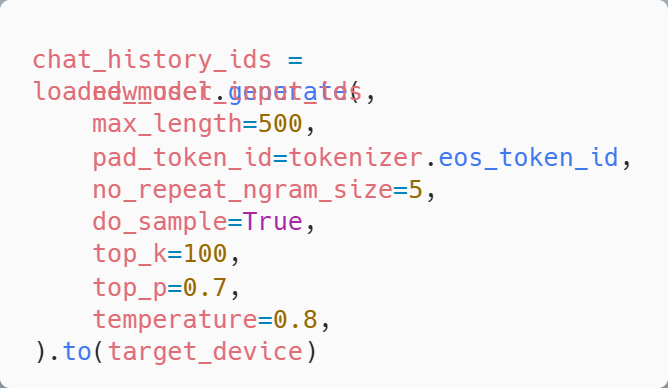
\includegraphics[width=0.8\textwidth]{fundation}}
	\caption{پیکربندی مدل}
	\label{fig:fundation}
\end{figure}

آزمایش‌های فرعی جهت ارزیابی قسمت‌های مختلف دخیل در فرآیند نماگر‌سازی کاربر به شرح زیر دسته‌بندی می‌شوند.
\begin{itemize}
\item
بدون ماژول تحلیل معنایی
\item
بدون فیلتر مشارکتی: صرف نظر از محاسبات شباهت و توصیه‌های مستقیم.
\item
ورودی توکن کاهش/افزایش‌یافته: مقایسه کیفیت کار و پیشنهادهای تولیدی سیستم زمانی که بیشینه طول عبارت تولیدی توسط سیستم کاهش یا افزایش باید.
\end{itemize}

در جدول 
\ref{tab:SensitivityAnalysis}
مقایسه تغییر مقادیر معیارهای ارزیابی معرفی‌شده با استفاده از مطالعات فرسایشی بر روی قسمت‌های مختلف سیستم آورده شده است.

% جدول مقایسه معیارهای ارزیابی با استفاده از مطالعات فرسایشی
\setlength{\extrarowheight}{0pt} % No extra space

\begin{table}[ht]
    \centering
    \caption{مطالعه فرسایشی}
    \label{tab:SensitivityAnalysis}
    \renewcommand{\arraystretch}{1} % Adjusts row height
    \onehalfspacing
    \begin{tabularx}{0.91\textwidth}{|
             >{\centering\arraybackslash}m{3.6cm}|
             >{\centering\arraybackslash}m{0.9cm}|
             >{\centering\arraybackslash}m{0.9cm}|
             >{\centering\arraybackslash}m{0.9cm}|
             >{\centering\arraybackslash}m{0.9cm}|
             >{\centering\arraybackslash}m{1.2cm}|
             >{\centering\arraybackslash}m{0.9cm}|
             >{\centering\arraybackslash}m{0.9cm}|} % Updated column count
        \hline
        \rotatebox{0}{معیارهای ارزیابی} & 
        \rotatebox{90}{Perplexity} &         
        \rotatebox{90}{ \text{\num{Distinct-1}}} & 
        \rotatebox{90}{ \text{\num{Distinct-2}}} & 
        \rotatebox{90}{\text{\num{SuccessRate}}} & 
        \rotatebox{90}{\text{\num{CompletionRate}}} & 
        \rotatebox{90}{UES} & 
        \rotatebox{90}{PDM} \\ % Ensure header matches columns
        \hline
        \rotatebox{0}{سیستم کامل} & 
        \textbf{\num{8.84}} &         
        \text{\num{0.26}} & 
        \text{\num{0.58}} & 
        \textbf{\num{91.97}} & 
        \textbf{\num{93.87}} & 
        \textbf{\num{91.97}} & 
        \textbf{\num{94.29}} \\
        \hline
        \rotatebox{0}{بدون تحلیل معنایی} & 
        \text{\num{9.50}} &         
        \text{\num{0.22}} & 
        \text{\num{0.5}} & 
        \text{\num{88}} & 
        \text{\num{90}} & 
        \text{\num{88}} & 
        \text{\num{91}} \\
        \hline
        \rotatebox{0}{بدون فیلتر مشارکتی} & 
        \text{\num{9.30}} &         
        \text{\num{0.24}} & 
        \text{\num{0.54}} & 
        \text{\num{89}} & 
        \text{\num{91}} & 
        \text{\num{89}} & 
        \text{\num{92.5}} \\
        \hline
        \rotatebox{0}{کاهش طول خروجی مدل} & 
        \text{\num{10.20}} &         
        \text{\num{0.18}} & 
        \text{\num{0.45}} & 
        \text{\num{85}} & 
        \text{\num{88}} & 
        \text{\num{85}} & 
        \text{\num{89}} \\
        \hline
        \rotatebox{0}{بدون پروفایل کاربری} & 
        \text{\num{11.50}} &         
        \textbf{\num{0.15}} & 
        \textbf{\num{0.4}} & 
        \text{\num{80}} & 
        \text{\num{83}} & 
        \text{\num{80}} & 
        \text{\num{85}} \\
        \hline
    \end{tabularx}
\end{table}





\subsection{تاثیر ماژول نماگر کاربری بر رضایت کاربران}
مشاهدات از مطالعات فرسایشی بخش نماگر سازی کاربربه شرح زیر است.

\subsubsection{ماژول تحلیل معنایی}

همانطور که انتظار می‌رفت، حذف برچسب‌گذاری احساسات باعث کاهش امتیازهای معیارهای ارزیابی مرتبط به نماگر کاربری شده‌است، زیرا نشانه‌های زمینه‌ای خاص ژانر یا برچسب از بین می‌رود.

معیار PDM زمانی که این مؤلفه حذف می‌شود، دقت و اثربخشی نماگر را کاهش می‌دهد. 

\subsubsection{ماژول فیلتر مشارکتی}

با حذف ماژول فیلتر مشارکتی مبتنی بر آیتم کاهش متوسط ​​در میزان موفقیت و تکمیل قابل مشاهده است، زیرا توصیه‌های شخصی‌شده حذف می‌شوند.
همچنین معیار PDM نشان‌دهنده کاهش جزئی به دلیل عدم وجود بینش مشترک بین نماگر کاربر و نتایج تولیدشده توسط مدل است.

\subsubsection{بدون هیچ‌ گونه نماگر کاربری}

بالاترین گیجی و کمترین UES، که منعکس‌کننده شخصی‌سازی و تعامل ضعیف است. معیار PDM در پایین‌ترین حد خود قرار دارد که نشان‌دهنده حداقل مشارکت در نماگر کاربری است.

\subsection{تاثیر کاهش طول بیشینه متن تولیدی توسط مدل}

تخریب قابل توجه در معیارهای تمایز و موفقیت به‌دلیل زمینه محدود برای تولید پاسخ، که ناشی از اتکای مدل به داده‌های ورودی گسترده‌تر و تولید متن طولانی‌تر برای حفظ انسجام و ایجاد پاسخ‌های متنوع است. این نشان می‌دهد که کاهش طول ورودی، توانایی مدل را برای استفاده مؤثر از داده‌های نماگر کاربر و تاریخچه گفتگو، و همچنین ارایه پیشنهاد در متن خروجی که برای تولید پاسخ‌های ظریف و شخصی‌شده حیاتی هستند، محدود می‌کند.


معیار PDM منعکس کننده تأثیر منفی گسترده‌تری بر تصمیمات نماگر است.

% \subsection{تاثیر استفاده از حق فراموشی در کیفیت خروجی مدل}



\subsection{جمع بندی}
ارزیابی های انجام شده نشان می‌دهد که چگونه تکنیک‌های نماگر کاربر به طور مستقیم با برجسته‌کردن تأثیر آنها بر معیارهایی مانند PDM و UES به عملکرد سیستم کمک می‌کند. 

این تجزیه و تحلیل همچنین زمینه‌های بالقوه برای بهینه‌سازی، مانند پالایش اجزای فیلتر مشارکتی یا تجزیه و تحلیل معنایی را روشن می‌کند و در نتیجه راه را برای تعامل کاربر افزایش‌ یافته و سیستم‌های گفتگوی قوی‌تر در آینده هموار می‌کند. ردیابی امتیاز PDM بینش بیشتری در مورد اثربخشی روش های نماگر ارائه می‌دهد. این یافته‌ها بهینه‌سازی بیشتر سیستم گفتگو و بهبود رضایت کاربر را راهنمایی می‌کند.

\section{نتایج نهایی و مقایسه با کارهای موجود}

\subsection{نتایج نهایی}
در این بخش با تاکید بر ایجاد یک سیستم گفتگوی شخصی با استفاده از تکنیک‌های تنظیم سریع و نماگر کاربری، عملکرد سیستم را از طریق معیارهای مختلفی ارزیابی کردیم. که کیفیت پاسخ های تولید‌شده، تعامل سیستم و رضایت کاربر را ارزیابی شده است. 

روش‌شناسی در اینجا شامل استفاده از سیستم‌های گفتگوی وظیفه‌گرا است که با تنظیم سریع بهبود یافته‌اند، جایی که مدل در طول زمان با ترجیحات کاربر سازگار می‌شود. برای ارزیابی عملکرد سیستم، مجموعه‌ای از معیارهای کلیدی را به کار می‌گیریم، از جمله:

نتایج نهایی و عملکرد روش پیشنهادی برای تمامی معیارهای کلیدی مورد ارزیابی در جدول%
\ref{tab:evaluationMetrics}
آمده است.

\begin{table}[ht]
    \caption{معیارهای ارزیابی و مقادیر آنها}
    \label{tab:evaluationMetrics}
    \centering
    \onehalfspacing
    \begin{tabularx}{0.5\textwidth}{|>{\centering\arraybackslash}X|>{\centering\arraybackslash}X|}
        \hline
        \rotatebox{0}{معیار} & 
        \rotatebox{0}{مقدار} \\ \hline
        Perplexity              & \num{8.84}         \\ \hline
        1Distinct               & \num{0.26}         \\ \hline
        2Distinct               & \num{0.58}         \\ \hline
        SuccessRate            & \num{91.97\%}       \\ \hline
        CompletionRate         & \num{93.87\%}       \\ \hline
        UES                     & \num{91.97}       \\ \hline
        PDM                     & \num{94.29}       \\ \hline
    \end{tabularx}
\end{table}


\subsection{مقایسه با کارهای موجود}

در این بخش، عملکرد روش پیشنهادی با کارهای موجود مقایسه شده است. از آنجایی که هیچ مرجعی وجود ندارد که شامل تمام معیارهای ارزیابی خاص ما باشد، مقایسه‌ها بر اساس معیارهای مشترک بین مقالات مختلف انجام شده است. به عبارت دیگر، هر مرجع تنها شامل بخشی از معیارهای ارزیابی است و ما عملکرد خود را با هر مرجع در معیارهای مربوطه مقایسه کرده‌ایم. مقایسه فوق در شکل%
\ref{fig:evaluationMetrics}
آمده است که در ادامه به طور جزیی تر مورد بحث قرارگرفته است.

\begin{figure}[ht]
    \centerline{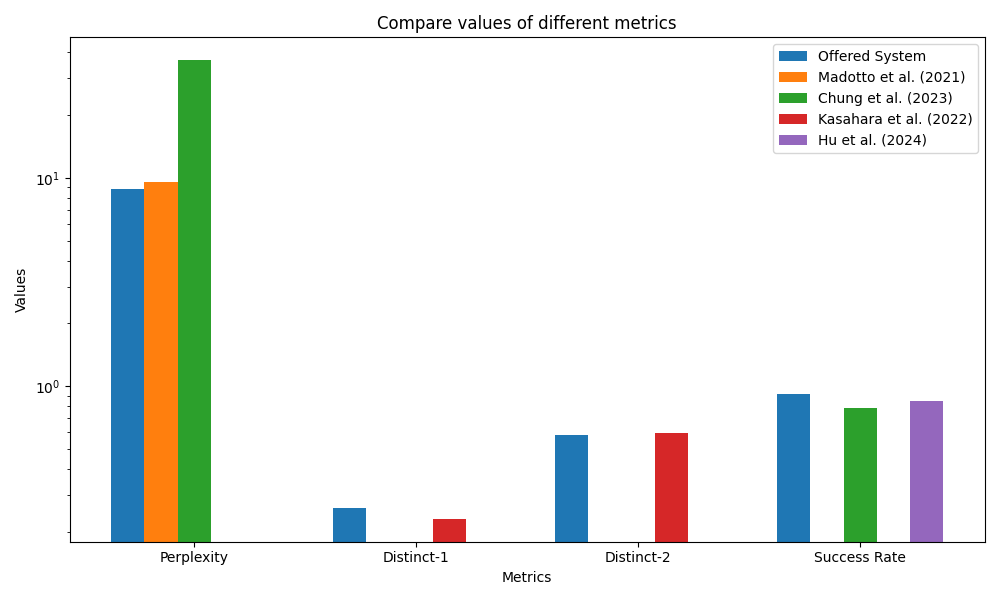
\includegraphics[width=1\textwidth]{evaluationMetrics}}
    \caption{مقایسه مقادیر معیارهای ارزیابی با کارهای موجود}
    \label{fig:evaluationMetrics}
\end{figure}
\begin{enumerate}
\item
گیجی: گیجی  روش پیشنهادی مقدار 
 \num{8.84}
 است که کمتر از مدل بیان‌شده در مقاله %
\cite{madotto2021few}
با مقدار
\num{9.5}
 و همچنین کمتر از مقدار بیان‌شده در مقاله %
\cite{chung2023instructtods}
با مقدار 
\num{36.63}
است، که نشان می‌دهد مدل در مقایسه با مقالات بیان‌شده در پیش‌بینی‌های خود اطمینان بیشتری دارد. این اختلاف می‌تواند به دلیل ماهیت خاص دامنه و بهبودهای انجام شده هنگام تنظیم سریع مدل باشد.

\item
معیار دیستینک-1: امتیاز مدل بیان شده 
 \num{0.26}
 است که با امتیاز گزارش شده در مقاله%
\cite{kasahara2022building}
\num{0.231}
 مطابقت دارد. این نشان می‌دهد که مدل فوق نسبت به تعداد کل تک‌گرم‌ها، یونی‌گرام‌های منحصربه‌فرد بیشتری تولید می‌کند، که نشان‌دهنده تنوع واژگانی بالاتر در سطح یونیگرام است.

\item
معیار دیستینک-2: مقاله 
\cite{kasahara2022building}
در مقایسه با کار مدل بیان شده با امتیاز 
\num{0.58}
 دارای امتیاز کمی بالاتر 
\num{0.595}
است. این نشان می‌دهد که مدل این مقاله نسبت به تعداد کل بای گرام‌ها، بای گرام‌های منحصربه‌فرد بیشتری تولید می‌کند که نشان‌دهنده تنوع واژگانی اندکی بالاتر در سطح بای‌گرام است.

\item
میزان موفقیت: میزان موفقیت در  روش پیشنهادی 
\num{91.79}
 متفاوت از آنچه در InstructTODS ارائه شده است.
مقاله «InstructTODS: مدل‌های زبان بزرگ برای سیستم‌های گفتگوی وظیفه‌گرا انتها به انتها»
\cite{chung2023instructtods}
 نرخ موفقیت را به عنوان معیاری از توانایی سیستم گفتگو برای دستیابی به هدف کاربر تعریف می‌کند. بر این اساس محاسبه می‌شود که آیا سیستم وظیفه درخواست‌شده توسط کاربر را با موفقیت انجام می‌دهد یا خیر. این مقاله مقدار نهایی
\num{78.48}
را برای میزان موفقیت خود ارایه داده است.

همچنین در 
\cite{hu2024dialight}
این مقدار به صورت میانگین برابر با 
\num{85.1}
محاسبه می‌شود. 


برای معیارهایی مانند میزان موفقیت، که در آن آثار مختلف از تعاریف متفاوتی استفاده می‌کنند تفاوت در روش‌های محاسبه باید مورد توجه قرار گیرد، زیرا ما از یک تعریف سفارشی بر اساس تکمیل کار استفاده می‌کنیم، در حالی که InstructTOD ممکن است شامل عوامل اضافی باشد اما تعریف نهایی همه در حیطه به انجام ‌رساندن وظیفه محول‌شده به سیستم گفتگو یکسان است.

در ارزیابی فوق میزان موفقیت را بر اساس تعداد کارهایی که با موفقیت توسط سیستم انجام شده است، با توجه به تشخیص قصد و دقت پاسخ محاسبه می‌کنیم.

\end{enumerate}


\subsection{ارزیابی انسانی}
علاوه بر ارزیابی‌های انجام شده، یک ارزیابی انسان-هوش مصنوعی انجام شده است که در آن ده ارزیاب انسانی با  روش پیشنهادی تعامل داشتند و در مورد جنبه‌های مختلف عملکرد سیستم بازخورد ارائه می‌کردند. در زیر نتایج آماری برای بازخورد انسانی آورده شده است.

ارزیابی انسانی به فرآیند ارزیابی خروجی های سیستم های توصیه از طریق قضاوت مستقیم انسانی اشاره دارد. این رویکرد به‌ویژه برای ارزیابی جنبه‌های کیفی توصیه‌ها، مانند ارتباط، انسجام، شخصی‌سازی و رضایت کاربر، که ممکن است معیارهای خودکار به‌طور کامل نتوانند از آن‌ها استفاده کنند، مهم است. ارزیاب‌های انسانی معمولاً توصیه‌ها را بر اساس معیارهای از پیش تعریف‌شده رتبه‌بندی یا رتبه‌بندی می‌کنند و بینش‌هایی را در مورد اینکه چقدر سیستم با انتظارات و نیازهای کاربر همسو می‌شود، ارائه می‌دهند.

برای مثال، در سیستم‌های توصیه مبتنی بر LLM، ارزیاب‌های انسانی ممکن است ارزیابی کنند که آیا آیتم‌های توصیه‌شده (مانند فیلم‌ها، محصولات یا مقالات) برای کاربر هدف مناسب، متنوع و جذاب هستند یا خیر %
\cite{elangovan2024considers}
.
نتایج ارزیابی‌های انسانی انجام‌شده به همراه ارسال همان سوالات و پاسخ‌ها به مدل هوش مصنوعی جی‌پی‌تی 
\num{3.5}
جهت انجام ارزیابی هوشمند و مقایسه آن در جدول 
\ref{tab:ComparisonGPT35}
آورده شده است.
\begin{table}[ht]
    \caption{مقایسه نتایج ارزیابی انسان و مدل}
    \label{tab:ComparisonGPT35}
    \centering
    \onehalfspacing
    \begin{tabularx}{\textwidth}{|>{\centering\arraybackslash}X|>{\centering\arraybackslash}X|>{\centering\arraybackslash}X|}
        \hline
        \rotatebox{0}{معیارها} & 
        \rotatebox{0}{ارزیابی انسان} &         
        \rotatebox{0}{ارزیابی هوش مصنوعی}  \\
        \hline
        \rotatebox{0}{Perplexity} & 
        \num{13.49} &         
        \num{13.09} \\
        \hline
        \rotatebox{0}{1Distinct} & 
        \num{0.29} &         
        \num{0.29} \\
        \hline
        \rotatebox{0}{2Distinct} & 
        \num{0.60} &         
        \num{0.60} \\
        \hline
        \rotatebox{0}{SuccessRate} & 
        \num{84.42} &         
        \num{85.29}\\
        \hline
        \rotatebox{0}{CompletionRate} & 
        \num{94.19} &         
        \num{93.89}  \\
        \hline
        \rotatebox{0}{UES} & 
        \num{79.57} &         
        \num{85.29}  \\
        \hline
    \end{tabularx}
\end{table}

\begin{itemize}
\item
گیجی: ارزیابی انسان برای گیجی تقریباً با نتایج مدل هوش‌مصنوعی یکسان است.
این نشان می‌دهد که پاسخ‌های این مدل برای انسان‌ها به همان اندازه که برای خود سیستم هوش‌مصنوعی گیج‌کننده است.
\item
دیستنیک ۱و ۲: هر دو معیار بین ارزیابی‌های انسان و هوش‌مصنوعی سازگار هستند، که نشان می‌دهد این مدل پاسخ‌های مشابهی را در تعاملات انسانی ایجاد می‌کند که در ارزیابی‌های هوش‌مصنوعی انجام می‌دهد.
\item
میزان موفقیت: میزان موفقیت در ارزیابی انسانی در مقایسه با نتایج مدل هوش‌مصنوعی کمی کمتر است. این اختلاف را می‌توان به ماهیت ذهنی ارزیابی انسانی نسبت داد، جایی که کاربران ممکن است همیشه در مورد تکمیل کامل یک کار به توافق نرسند.
\item
نرخ تکمیل: میزان تکمیل در هر دو ارزیابی تقریباً یکسان است، با یک تفاوت بسیار کوچک، که نشان می‌دهد سیستم در هر دو ارزیابی پاسخ‌های منسجم و کاملی را ارائه می‌دهد.
\item
 امتیاز تعامل کاربر: در ارزیابی انسانی در مقایسه با هوش‌مصنوعی به طور قابل ‌توجهی کمتر است. این اختلاف ممکن است منعکس‌کننده تفاوت در نحوه درک ارزیابی‌های انسانی از کیفیت تعامل در مقابل ارزیابی داخلی مدل هوش‌مصنوعی باشد.
\end{itemize}

بازخورد انسانی نشان می‌دهد که در حالی که مدل هوش‌مصنوعی در ایجاد پاسخ‌ها عملکرد خوبی دارد، تفاوت‌های ظریفی در نحوه درک انسان از اثربخشی سیستم، به ویژه در مورد تعامل کاربر وجود دارد. این بینش، پیشرفت‌های آینده را در افزایش توانایی سیستم برای تعامل مؤثرتر با کاربران راهنمایی می‌کند.

\subsection{رابط‌کاربری برای ارزیابی انسانی}

برای ارزیابی اثربخشی سیستم گفتگوی وظیفه‌گرا و جمع‌آوری بازخورد انسانی، یک رابط کاربری مبتنی بر اپلیکیشن موبایل نیز توسعه داده شد. این رابط کاربری برای تقلید از سناریوهای دنیای واقعی طراحی شده است که در آن کاربران با سیستم‌های توصیه‌ای تعامل دارند و به آنها اجازه می‌دهد:
\begin{itemize}
\item
ثبت ٰژانرهای مورد علاقه: برای همه کاربران به‌ویژه برای کاربران تازه وارد، امکان انتخاب ژانرهای مورد علاقه فراهم است.
\item
 ارسال پرسش‌ها: کاربران عبارت‌های زبان طبیعی را وارد می‌کنند، مانند «آیا می‌توانید یک فیلم اکشن توصیه کنید؟»
\item
 دریافت پاسخ‌ها: سیستم توصیه‌های سریع تنظیم‌شده متناسب با پرس‌و‌جو و نماگر کاربر را ارائه می‌دهد.
\item
 ارائه بازخورد: کاربران می‌توانند با انتخاب یکی از سه گزینه به پاسخ‌ها واکنش نشان دهند: «پسندیدن»، «نپسندیدن» یا «خنثی».
\end{itemize}

هدف اولیه رابط کاربری ارزیابی عملکرد سیستم از نظر موارد زیر بود:
\begin{itemize}
\item
 ارتباط و انسجام: توسط بازخورد کاربر در مورد پاسخ‌های فردی ارزیابی می‌شود.
\item
 تعامل و رضایت: از طریق تعاملات مکرر و ورودی کیفی کاربر اندازه گیری می‌شود.
\item
 تنوع پاسخ: با مشاهده واکنش کاربران به ژانرها یا سبک‌های مختلف پاسخ‌ها ارزیابی می‌شود.
\end{itemize}

این رابط همچنین ثبت تمام تعاملات کاربر را تسهیل کرد و یک مجموعه داده حیاتی را برای ارزیابی انسانی تشکیل داد. این مجموعه، داده برای محاسبه معیارهایی مانند امتیاز تعامل کاربر و میزان موفقیت و اعتبارسنجی معیارهای خودکار استفاده شد.

یک نمونه از این رابط کاربری مطابق با شکل%
\ref{fig:MindMeldUi}
 است.

\begin{figure}[ht]
	\centerline{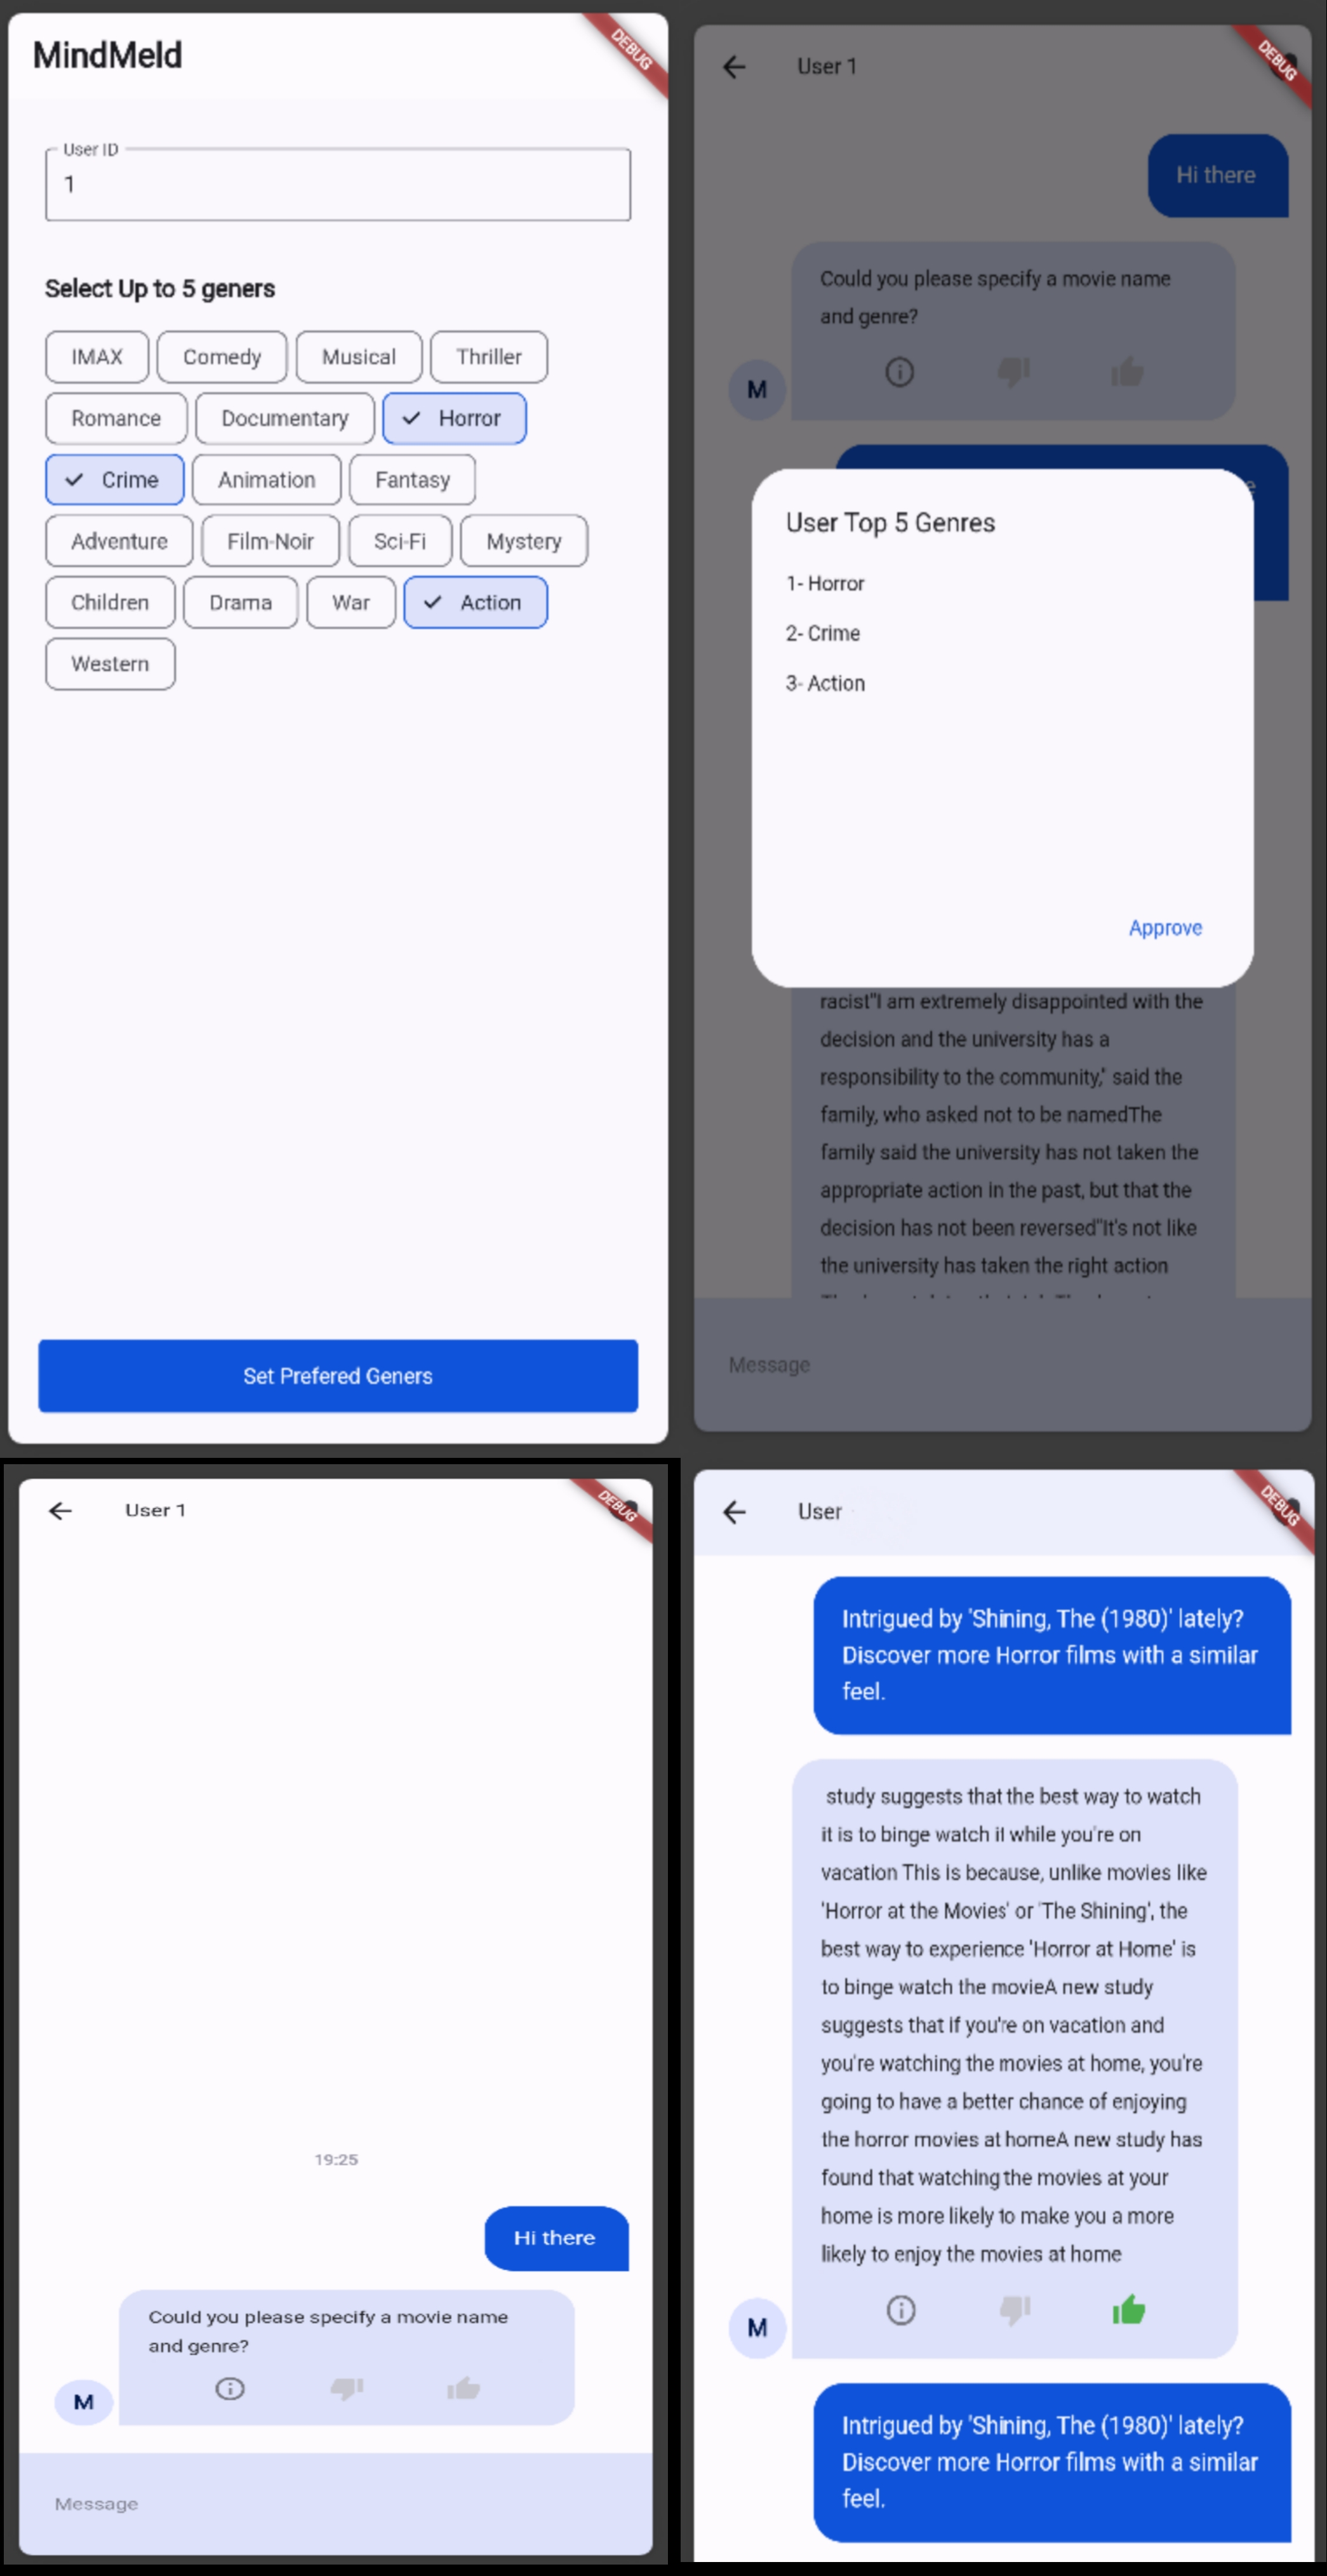
\includegraphics[width=0.5\textwidth]{prototype}}
	\caption{رابط کاربری طراحی‌شده}
	\label{fig:MindMeldUi}
\end{figure}



\section{نتیجه‌گیری}

در این فصل، به طور سیستماتیک مجموعه داده‌های مورد استفاده برای آموزش و ارزیابی مدل را با تمرکز اولیه روی مجموعه داده‌های مووی‌لنز مورد بررسی قرار گرفت. 

این مجموعه داده‌های غنی و متنوعی از تعاملات کاربران ارائه می‌دهد که مبنایی برای کارهای شخصی‌سازی و توصیه‌ها را تشکیل می‌دهد. ویژگی‌های مجموعه داده‌ها، از جمله رتبه‌بندی‌های کاربر، ژانرهای فیلم، و مُهرهای زمانی را که برای ایجاد نماگر‌های دقیق کاربر ضروری بودند، به تفصیل شرح داده شدند. 

مجموعه داده‌های آزمایشی به دقت تنظیم شدند تا عملکرد مدل را تحت سناریوهای واقعی ارزیابی کنند و از مقایسه منصفانه و قابل اعتماد نتایج اطمینان حاصل کنند. علاوه بر این، این فصل در مورد پیکربندی ابرپارامتر که برای افزایش کارایی مدل، از جمله نرخ یادگیری به خوبی تنظیم شده بودند، توضیح داده‌شد.

نتایج با استفاده از معیارهایی مانند گیجی، تمایز، میزان موفقیت، میزان تکمیل و امتیاز تعامل کاربر و همچنین معیارهای مرتبط به طور مستقیم با نماگر کاربری مانند دقت توصیه شخصی و تطابق تنوع نماگر ارزیابی شدند. 

این معیارها نقاط قوت و محدودیت‌های مدل را برجسته می‌کنند و نمای شفافی از عملکرد آن در ابعاد مختلف ارائه می‌دهند. تجزیه و تحلیل حساسیت بیشتر استحکام مدل را در برابر تغییرات در پارامترهای کلیدی نشان داد و بر سازگاری و قابلیت اطمینان آن در محیط‌های پویا تأکید کرد. 

این فصل چارچوب آزمایش و ارزیابی دقیق را در بر می‌گیرد که از نتیجه‌گیری‌ها و بینش‌های گسترده‌تر ارائه‌شده در این تحقیق پشتیبانی می‌کند.

 روش پیشنهادی در بسیاری از زمینه‌ها خوب عمل می‌کند، اما فضایی برای بهبود، به ویژه در تعامل با کاربر، همانطور که توسط ارزیابی انسان-هوش‌مصنوعی برجسته شده‌است، نشان می‌دهد.



		% فصل چهارم: نتایج
% !TeX root=../main.tex
\chapter{[جمع بندی و پیشنهادهایی برای ادامه پژوهش]}
%\thispagestyle{empty} 
\section{مقدمه}

\section{اهداف تحقیق}
هدف این رساله، بهبود سیستم‌های گفتگوی وظیفه‌محور با مقابله با چالش‌ها در شخصی‌سازی، نمایه‌سازی کاربر، مشکل شروع سرد و در عین حال تضمین حریم خصوصی از طریق رعایت حق فراموشی بود. 

با استفاده از تکنیک هایی مانند تنظیم سریع، فیلتر مشارکتی، و پروفایل پویا کاربری، پیشرفت‌های قابل‌توجهی از نظر دقت سیستم، سازگاری و رضایت کاربر به دست آمد.

\subsection{نتایج کلیدی}

\subsubsection{پیشرفت در شخصی سازی}
\begin{itemize}
\item
تولید دیالوگ تطبیقی:
 
سیستم گفتگو با ترکیب ترجیحات کاربر مانند ژانرهای مورد علاقه، تعاملات گذشته و ویژگی‌های خاص زمینه، پاسخ‌های خود را به صورت پویا تنظیم می‌کند. به عنوان مثال کاربرانی که فیلم‌های علمی تخیلی را ترجیح می‌دهند، توصیه‌ها و تعاملات غنی‌شده با زبان مرتبط را دریافت کردند که به طور قابل‌توجهی امتیاز تعامل آنها را بهبود بخشید.

همچنین نمرات گیجی و تمایز بهبود‌یافته تعادل بین ارتباط و تنوع پاسخ را نشان می‌دهد.
\item
 تنظیم سریع برای شخصی‌سازی:
 این رویکرد اجازه کنترل دقیق بر پاسخ‌های سیستم را بدون آموزش مجدد کل مدل می‌دهد. همچنین با استفاده از این روش می‌توان به قابلیت‌های یادگیری چند شات دست یافت و سیستم را قادر ساخت حتی با داده‌های محدود به خوبی تعمیم یابد.
استفاده از این روش، از روش‌های تنظیم دقیق سنتی با کاهش سربار محاسباتی و در عین حال حفظ تعاملات با کیفیت بالا و مرتبط با زمینه، عملکرد بهتری داشت.
\end{itemize}
\subsubsection{حل مشکل شروع سرد}
سیستم با استفاده نوآورانه از فیلتر مشارکتی تعاملات اولیه با کاربران با استفاده از فیلتر اشتراکی مبتنی بر آیتم را افزایش داده‌ها از کاربران مشابه برای شخصی‌سازی به طرز محسوسی افزایش یافت.

در نتیجه سیستم به طور موثر مشکل شروع سرد را برطرف کرد و توصیه‌های دقیق و تعاملات معناداری را برای کاربران جدید ارائه کرد.

\subsubsection{متریک و ارزیابی}
 معیارهای ارزیابی مختلفی مورد بحث قرارگرفت. این سیستم با استفاده از معیارهایی مانند گیجی، تمایز، میزان موفقیت، نرخ تکمیل کار و میزان درگیری کاربر به شدت مورد ارزیابی قرار گرفت.
\begin{itemize}
\item
 گیجی: نمرات پایین‌تر توانایی بهبودیافته سیستم را برای ایجاد پاسخ‌های منسجم و مرتبط با زمینه نشان می‌دهد.
\item
 تمایز: افزایش قابل‌بیانی را نشان داد که نشان‌دهنده تنوع بیشتر در پاسخ‌های ایجاد شده است.
\item
 امتیاز تعامل کاربر : با انطباق پویا با پروفایل‌های کاربر و نرخ تکمیل کار بهبود یافته‌است.
\item
 میزان موفقیت کار: در میان پرس‌وجوهای مختلف، این سیستم در مقایسه با سیستم‌های گفتگوی وظیفه‌محور ذکر شده، هشت الی 17 درصد پیشرفت در موفقیت کار به دست آورد. تجربه کاربری شخصی‌سازی‌شده به طور قابل‌توجهی به این موفقیت کمک کرد.
\end{itemize}
\subsection{ادغام حق فراموشی و حریم خصوصی}
این سیستم نگرانی‌های فزاینده در مورد حفظ حریم خصوصی در حوزه‌ي داده‌ها را از طریق رعایت حق فراموشی برطرف کرد.

 حذف پویا اطلاعات کاربر مکانیسم‌هایی را برای کاربران به منظور درخواست حذف داده‌های خود پیاده‌سازی کرده است، که از عدم وجود اثر باقی‌مانده در پروفایل‌های کاربر یا سیستم‌های فیلتر مشترک اطمینان حاصل می‌کند. این ویژگی اعتماد کاربر را افزایش داد و با قوانین حفظ حریم خصوصی جهانی هماهنگ شد و معیاری برای سیستم‌های هوش مصنوعی اخلاقی تعیین کرد. علیرغم حذف داده‌های کاربر، تنظیم سریع و یادگیری چند شات به سیستم اجازه می‌دهد تا عملکرد بالایی را بدون اتکا به داده‌های تاریخی حفظ کند.

\subsection{سازگاری با دامنه های جدید}

 انعطاف‌پذیری در استفاده از پایگاه دانش برای سیستم فوق نیز قابل بیان است.

 می‌توان از قابلیت انطباق مدل‌های زبانی با هر پایگاه دانشی استفاده کرد و از ارتباط سیستم در حوزه‌های مختلف اطمینان حاصل کرد. در صورت وجود دیتاست‌ مرتبط با هرحوزه، سیستم را می‌توان به راحتی به برنامه‌های کاربردی خدمات مشتری، مراقبت‌های بهداشتی و تجارت الکترونیک گسترش داد.

همچین تکنیک‌های شروع سرد و آموزش چندشات، سیستم را قادر می‌سازد حتی در سناریوهایی که قبلاً دیده نشده بود یا با حداقل داده‌های مربوط به کار، به خوبی عمل کند و نیاز به بازآموزی گسترده را به حداقل برساند.

\subsection{زمینه‌های فراگیر}

\begin{itemize}
\item
رضایت و تعامل کاربر

 شخصی‌سازی و رعایت حریم خصوصی به طور جمعی رضایت کاربر را افزایش می‌دهد، همانطور که با نمرات تعامل بالاتر مشهود است.
 تعادل بین حریم خصوصی و عملکرد استاندارد جدیدی را برای سیستم‌های هوش مصنوعی در حوزه‌های تنظیم‌شده ایجاد می‌کند.
\item
مقیاس پذیری

ماهیت سبک تنظیم سریع مقیاس‌پذیری را در دستگاه‌های با قدرت محاسباتی محدود تضمین می‌کند و این رویکرد را برای مخاطبان گسترده‌تری قابل دسترسی می‌سازد.
\item
حفظ حریم خصوصی

گنجاندن انطباق با حق فراموشی، همسویی سیستم را با شیوه‌های هوش‌مصنوعی اخلاقی برجسته می‌کند و به مسائل مربوط به اعتماد کاربر که اغلب در سیستم‌های گفتگوی وظیفه‌محور سنتی نادیده گرفته می‌شوند، می‌پردازد.
\end{itemize}

\section{مشارکت و نوآوری}
این رساله از سیستم‌های گفتگوی وظیفه محور، با تمرکز بر شخصی سازی،شروع سرد و حفظ حریم خصوصی، در حالی که از تکنیک های نوآورانه مانند تنظیم سریع و ساخت پروفایل کاربری با استفاده از تکنیک‌هایی مانند فیلتر مشارکتی مبتنی بر آیتم و تحلیل احساسات استفاده می کند.

در زیر یک طرح کلی ساختار یافته از مشارکت ها و جنبه های بدیع این تحقیق آورده شده است.

\subsection{مشارکت های اصلی}
\subsubsection{شخصی سازی در سیستم های گفتگو}


\begin{itemize}
\item
 پروفایل کاربری پویا:

 یک چارچوب جدید برای ایجاد و حفظ نمایه‌های کاربر پویا با استخراج اولویت‌ها (مانند ژانرهای برتر، فیلم‌های پسندیده) از تعاملات ایجاد شد.

در نتیجه سیستم پاسخ‌ها را در زمان واقعی تطبیق داده و تعامل و رضایت کاربر را بهبود می‌بخشد.

برخلاف سیستم‌های شخصی‌سازی ایستا یا مبتنی‌بر قانون، این رویکرد یادگیری و سازگاری مداوم را امکان‌پذیر می‌کند که پروفایل هرکاربر به مرور و با تعامل با برنامه به‌روز شود.
\item
 تعاملات آگاه از زمینه:

استفاده از تنظیم سریع امکان ادغام بلادرنگ زمینه کاربر (به عنوان مثال، ترجیحات، تاریخچه هر گفتگو) را در پاسخ‌های سیستم فراهم می‌کند. با اتکا به این روش افزایش ارتباط و انسجام در گفتگو ایجاد شده‌است که با نرخ موفقیت بالاتر و معیارهای تعامل این پیشرفت نشان داده شده‌است.
\item
پرداختن به مشکل شروع سرد:

این سیستم علاوه بر ژانرهای دریافتی مورد علاقه کاربر نوپا، فیلتر مشارکتی مبتنی بر آیتم را برای مدیریت مشکل شروع سرد با استفاده از داده‌های کاربران مشابه پیاده‌سازی کرده است.

این رویکرد با موفقیت شکاف را برای کاربران جدید پر می‌کند و از تعاملات معنی‌دار حتی با حداقل داده‌های اولیه اطمینان حاصل می‌ند. این عملکرد جهت حل مشکل شروع سرد در سیستم نشان می‌دهد که فیلتر کردن مشارکتی می‌تواند فراتر از سیستم‌های توصیه گسترش یابد تا شخصی‌سازی گفتگو را بهبود بخشد.
\item
 آموزش چند شات:

 این تکنیک‌ها را برای مدیریت مؤثر سناریوهای نادیده، به حداقل رساندن نیاز به داده‌های گسترده ویژه کار، به کار گرفت.
به همین علت امکان استقرار سریع سیستم های گفتگو در حوزه‌های جدید بدون آموزش مجدد فراهم آمده است.
\end{itemize}


\subsubsection{حریم خصوصی و هوش مصنوعی اخلاقی}

\begin{itemize}
\item
 حق فراموش شدن:

در این رساله مکانیسم‌هایی برای انطباق با حق فراموشی استفاده شد که به کاربران اجازه می‌دهد بدون تأثیر بر عملکرد سیستم، درخواست حذف داده‌های خود را داشته باشند.

این یکی از پیاده‌سازی‌های سیستم‌های گفتگوی وظیفه محور است که انطباق حق فراموشی را با حفظ عملکرد عملیاتی می‌کند. با ایجاد این مهم، اعتماد کاربر جهت استفاده از سیتسم افزایش یافته و با قوانین جهانی حفظ حریم خصوصی داده‌ها هماهنگ می‌شود.
\item
 متعادل کردن حریم خصوصی و شخصی سازی:

روش‌های توسعه‌یافته برای ایجاد تعادل بین حریم خصوصی و شخصی‌سازی با اطمینان از اینکه داده‌های کاربر حذف شده عملکرد کلی سیستم را به خطر نمی‌اندازد. این تعادل امکان شخصی‌سازی حفظ حریم خصوصی در سیستم‌های هوش‌مصنوعی را در کنار قابلیت شخصی‌سازی‌کردن نتایج نشان داد.
\end{itemize}

\subsubsection{معیارها و چارچوب ارزیابی}
معیارهای ارزیابی پیشرفته:

یک چارچوب ارزیابی قوی با استفاده از گیجی، تمایز، میزان موفقیت، میزان تکمیل کار، امتیاز تعامل کاربر و همچنین دقت توصیه شخصی و تطابق تنوع نمایه معرفی شدند.
معیارهای فوق مجموعه ای جامع از معیارها را معرفی کرد که به طور خاص برای ارزیابی سیستم‌های گفتگوی وظیفه محور شخصی سازی شده و سازگار طراحی شده است.این معیارها روشی استاندارد برای ارزیابی عملکرد سیستم‌های گفتگوی وظیفه محور فراتر از معیارهای سنتی ارائه می‌کند.


\subsubsection{تکنیک ها و روش های بدیع}


\begin{itemize}
\item
 تنظیم سریع به عنوان یک روش اصلی:

 یک جایگزین سبک وزن و در عین حال قدرتمند برای تنظیم دقیق، تنظیم سریع برای دستیابی به شخصی‌سازی و سازگاری محوری بود.
 
استفاده از این روش، کارآمدی تنظیم سریع در تنظیم پویا دیالوگ‌ها بدون متحمل‌شدن هزینه‌های محاسباتی بالا را به نمایش گذاشت. همچنین تنظیم سریع به عنوان یک رویکرد قابل دوام برای سیستم‌های گفتگوی وظیفه محور ایجاد شد.

\item
 رویکرد ترکیبی برای شخصی سازی:

 ترکیبی از پروفایل کاربری، فیلترکردن مشارکتی و مدل‌های زبانی برای ایجاد یک سیستم ترکیبی که از نقاط قوت هر جزء استفاده می‌کند. این ترکیب روش‌ها و نتایج ارزیابی به خوبی نشان داد که چگونه مدل‌های ترکیبی می‌توانند از رویکردهای مستقل در شخصی سازی و رضایت کاربر بهتر عمل کنند.

\item
 ادغام هوش مصنوعی اخلاقی:

 به نگرانی‌های مربوط به حریم خصوصی و اخلاقی از طریق راه‌حل‌های نوآورانه پرداخته و استاندارد جدیدی برای شیوه‌های هوش مصنوعی اخلاقی در سیستم‌های گفتگو ایجاد می‌کند.
\end{itemize}


این تحقیق با پرداختن به چالش‌های قدیمی در شخصی‌سازی، سازگاری و رعایت حریم خصوصی، شکاف‌های حیاتی در توسعه سیستم‌های گفتگوی وظیفه‌محور را پر می‌کند. همچنین یک نقشه راه برای ادغام شیوه های هوش‌مصنوعی اخلاقی در سیستم‌های گفتگو ارائه کرد و تنظیم سریع به عنوان یک تکنیک اصلی برای سیستم‌های تطبیقی ​​و مقیاس‌پذیر ایجاد شد.


\section{پیشنهادهایی برای تحقیقات آینده}
این بخش مسیرهای بالقوه ای را برای کاوش بیشتر، بر اساس مبانی و یافته های این تحقیق بیان می‌کند. پیشنهادات زیر زمینه‌هایی را برای بهبود، گسترش و نوآوری در سیستم‌های گفتگوی وظیفه‌محور، شخصی‌سازی و هوش‌مصنوعی اخلاقی برجسته می‌کنند.

\subsection{پیشبرد تکنیک های شخصی سازی}

\subsubsection{پروفایل کاربری پیشرفته}

\begin{itemize}
\item
 پروفایل کاربری عمیق

 تحقیقات آینده می‌تواند تکنیک‌های پیچیده‌تر پروفایل‌سازی کاربر را بررسی کند، و همچین با بهره‌بردن از داده‌های چندوجهی مانند صدا، ویدیو یا فعالیت رسانه‌های اجتماعی کاربر، درک بهتری از ترجیحات کاربر ایجاد کند.
با استفاده از این روش‌ها شخصی‌سازی برای هر کاربر را فراتر از داده‌های صرفا متنی خواهد برد و نتیجه را بهبود می‌بخشد.
\item
 ترجیحات زمانی و متنی

 علاوه بر جنبه‌های متنوع پروفایل ‌کاربری می‌توان از اینکه چگونه ترجیحات کاربر در طول زمان تغییر می کند یا بر اساس زمینه های موقعیتی متفاوت است نیز جهت بهبود و ارتقای پروفایل کاربری استفاده کرد.
به عنوان مثال باید مدل‌های پویا را پیاده‌سازی کرد که از رفتار کاربر در بازه های زمانی مختلف یا در طول سناریوهای خاص یاد می گیرند و ترجیحات وی را به‌روز می‌کنند.
\end{itemize}

\subsubsection{فیلتر مشارکتی و ترکیبی}
می‌توان با کاوش روش‌های ترکیبی که فیلتر مشارکتی را با مدل‌های مبتنی بر یادگیری عمیق ترکیب می‌کند،مشکلات شروع سرد را به طور مؤثرتری مدیریت کرد.به عنوان مثال می‌توان با استفاده از تکنیک های مبتنی بر نمودار ارتباطات پنهان بین کاربران و آیتم ها را به طور موثرتر و بهتر شناسایی کرد.


\subsection{گسترش چارچوب های ارزیابی}

\begin{itemize}
\item
معیارهای جدید

همچنین می‌توان با تعریف معیارهای جدید، اندازه‌گیری میزان درک و پاسخ سیستم به احساسات کاربر را بیشتر و بهتر بررسی کرد. به عنوان مثال تعریف امتیاز درگیری عاطفی بر اساس احساسات و حالات عاطفی در پاسخ‌ها که سیستم با توجه به حال عاطفی کاربر پاسخ‌های متناسب به وی بدهد.
\item
 معیارهای خاص دامنه

 معیارهای ارزیابی برای حوزه‌های خاص (به عنوان مثال، دقت برای توصیه‌های پزشکی، ارتباط با توصیه‌های فیلم). در کارهای آتی می‌توان به تاثیر عمیق معیارهای دامنه خاص بر رضایت کاربر تمرکز کرد و آنرا بهبود داد.
\end{itemize}

\subsection{یکپارچه سازی مدل های پیشرفته}
\begin{itemize}
\item
ارتقاء مدل زبانی

با گنجاندن مدل‌های زبانی پیشرفته‌تر که پتانسیل آن‌ها را برای درک بهتر، تولید و شخصی‌سازی بیشتر است به طور حتمی نتایج بهتری در پی خواهد بود. ولی چالش استفاده از این مدل های زبانی حفظ تعادل هزینه محاسباتی با بهبود عملکرد سیستم خواهد بود.
\item
ادغام چندوجهی

ترکیب روش واکاوی متن با سایر روش‌های سیستم‌های توصیه مانند دیالوگ‌های مبتنی بر تصاویر، صدا و ویدئو برای تعاملات بیشتر با کاربر نیز می‌تواند جزو کارهای آتی قرار بگیرد. به عنوان مثال توصیه فیلم‌های دارای تریلر یا صحنه بر اساس ترجیحات کاربر می تواند در ارایه پیشنهادهای بهتر به کاربر موثر باشد.
\end{itemize}

پیشنهادات ذکر شده در بالا، پتانسیل قابل توجهی را برای توسعه بیشتر در سیستم‌های گفتگوی وظیفه‌محور، شخصی‌سازی و هوش‌مصنوعی حفظ حریم خصوصی نشان می‌دهد. با کاوش در این جهت‌ها، محققان آینده می‌توانند بر روی این کار برای افزایش رضایت کاربر، سازگاری سیستم و استقرار هوش مصنوعی اخلاقی کار کنند.


\section{محدودیت ها و چالش ها}

این بخش به طور انتقادی محدودیت‌ها و مشکلاتی را که در طول توسعه و ارزیابی سیستم گفتگوی وظیفه‌محور با نمایه‌های شخصی‌شده و تنظیم سریع مواجه می‌شود، بررسی می‌کند. محدودیت‌ها حوزه‌هایی را برجسته می‌کنند که بر نتایج تأثیر گذاشتند و بینش‌هایی را در مورد چالش‌هایی که باید برای بهبود بیشتر مورد توجه قرار گیرند، ارائه می‌دهند.

\subsection{محدودیت داده ها}
محدودیت های مجموعه داده به شرح زیر است.
\begin{itemize}
\item
 تولید داده های سفارشی

به دلیل عدم وجود مجموعه داده‌های مکالمه‌ای که از قبل برای توصیه‌های فیلم طراحی شده‌اند، زمان و تلاش قابل توجهی برای ایجاد مجموعه‌ای که داده‌های مکالمه را تقلید می‌کند، صرف شد. داده‌های تولید شده، اگرچه مؤثر هستند، ممکن است فاقد تنوع و عمق مکالمات در دنیای واقعی باشند به دلیل آنکه در نهایت این مکالمات ساختی و با استفاده از قالب و الگوهای از پیش تعیین‌شده هستند که نمی‌توانند با تنوع مکالمات واقعی مقایسه گردد. با بهبود و ارتقای این مجموعه داده، پاسخ‌های متنوع‌تر و با ترکیب کلمات بهتر ایجاد خواهد شد.

\item
 حجم داده محدود برای تنظیم دقیق

حجم داده‌های تولیدشده برای تنظیم دقیق مدل زبانی در مقایسه با مقیاس داده‌های مورد استفاده برای آموزش مدل های زبانی بزرگ محدود بود و همین باعث کاهش تعمیم‌پذیری و سازگاری مدل و عدم اجرای عملیات تنظیم دقیق بر روی مدل شده است.
\end{itemize}

\subsection{محدودیت های محاسباتی}
برای استفاده از مدل‌های زبانی آموزش آنها و اجرای تکنیک‌های مختلف، سخت‌افزار عضو جدایی ناپذیر از این عملیات است. 

\begin{itemize}
\item
محدودیت های منابع سخت افزاری

 اتکا به پردازنده‌های گرافیکی، اندازه مدل، اندازه دسته‌ای و تکرارهای آموزشی را محدود می‌کرد. به عنوان مثال به دلیل داشتن منابع سخت‌افزاری محدودتر ، اجبار به استفاده از مدل‌های زبانی با پارامترهای کمتر به جای مدل های پیشرفته تر مانند جی‌پی‌تی۴ باعث عدم دسترسی به نتایج بهتر شد.

\item
 محدودیت های زمانی

 چرخه‌های تمرین و تنظیم دقیق به دلیل محدودیت‌های زمانی غیرعملی بود که بر بهینه‌سازی و آزمایش هایپرپارامتر تأثیر گذاشت.
\end{itemize}


\subsection{چالش های پروفایل کاربری}
\begin{itemize}
\item
مشکل شروع سرد

برای کاربرانی که تازه با سیتسم شروع با کار می‌کنند، داده‌های تاریخی محدود است و می‌بایست توصیه‌های شخصی‌سازی‌شده را در ابتدا دقیق‌تر کرد تا برای این دسته کاربران نیز نتایج قابل قبولی ارایه شود. با استفاده از فیلتر مشارکتی و استفاده از اولویت‌های پیش‌فرض ژانر تا حدی این مشکل را برطرف شد.

\item
تحول تنظیمات کاربر در مرور زمان اگر در سیستم اعمال نشود باعث کاهش رضایت کاربر خواهد شد. تکنیک‌های پروفایل پویا برای انطباق با تغییر سلیقه کاربر در طول زمان تلاش کردند تا به حل این مشکل بیایند. لذا با ترکیب مدل‌های پروفایل کاربر پویا با قابلیت‌های یادگیری افزایشی و دریافت بازخورد مناسب از کاربر و به‌روزرسانی ترجیحات وی می‌توان از این مشکل جلوگیری کرد.
\end{itemize}

\subsection{نگرانی های حفظ حریم خصوصی}
پیاده سازی حق فراموشی در سیستم‌‌های گفتگو دارای پیچیدگی‌هایی است. اگرچه حق فراموشی اجرا شد، فرآیند حذف ایمن داده‌های کاربر بدون تأثیر بر مدل جهانی نیازمند تلاش قابل توجهی بود. همچنین می‌توان با کاوش در رویکردهای غیرمتمرکز برای افزایش حریم خصوصی داده ها این پیاده‌سازی را به صورت موثرتر پیاده‌سازی کرد و آن‌را بهبود داد.


\subsection{چالش های ارزیابی}
معیارهای ارزیابی سیستم‌های گفتگو به طور کلی ماهیت ذهنی دارند. معیارهایی مانند رضایت کاربر و امتیازات تعامل به بازخورد ذهنی بستگی دارد که ممکن است بین کاربران متفاوت باشد. که این ماهیت ذهنی مشکل در نتیجه گیری قابل اجرا جهانی را در پی خواهد داشت.

همچنین معیارهای مرسوم دیگر نیازمند یک جواب خاص یا جواب طلایی جهت مقایسه جواب نهایی مدل با آن جواب طلایی بودند ولی در سیستم‌های گفتگو که با مدل‌های زبانی کار می‌کنند ممکن است جواب مدل درست باشد ولی از جواب طلایی که مبنای امتیازدهی است متفاوت باشد.

به همین علت باید معیارهای جامع‌تر که هم مجزا از پاسخ طلایی و هم مقداری خارج از ماهیت ذهنی کاربران باشد مانند نرخ تکمیل کار یا نرخ کلیک یا میزان درگیربودن کاربر در مکالمه ایجاد کرد.

\subsection{محدودیت های مدل}
اندازه و معماری مدل با توجه به استفاده از مدل زبانی با پارامترهای کمتر انتخاب شد. در حالی که مدل زبانی مورد استفاده برای محدوده این پروژه کافی بود، عملکرد و درک متنی آن نسبت به مدل های بزرگتر مانند جی‌پی‌تی۴ یا لاما۳ پایین‌تر بود. استفاده از مدل با پارامترهای کمتر منجر به پاسخ‌های کم‌تر و کوتاه‌تر انسجام در نتیجه نتایج ناکارآمدتر خواهدشد.


\subsection{چالش های تنظیم سریع}
پاسخ‌های نهایی مدل و نتایج ارزیابی آن به کیفیت تنظیم سریع بسیار وابسته است. همچنین عملکرد مدل‌های تنظیم‌شده سریع به کیفیت درخواست‌های ورودی بسیار حساس بود. به طور مثال دستورات بد ساخته‌شده منجر به خروجی‌های مدل غیربهینه شد.

علاوه بر آن علیرغم بهبودهایی که از طریق تنظیم سریع انجام شد، این مدل قابلیت‌های محدودی را در سناریوهای شات صفر نشان داد. با استفاده از رویکردهای فرایادگیری برای بهبود سازگاری می‌توان این مشکل را به حداقل رساند.

\subsection{شخصی سازی پاسخ پویا}

تنظیم پویا پاسخ‌ها بر اساس بازخورد کاربر در حال تکامل، چالش‌هایی را در حفظ انسجام و ارتباط پاسخ ایجاد می‌کند.
برای بهبود عملکرد این بخش باید طراحی حلقه های بازخورد بلادرنگ برای پاسخ های تطبیقی بهبود یافته و به طور موثرتر در سیستم پیاده سازی شوند.

محدودیت‌ها و چالش‌هایی که بیان شد، بر پیچیدگی‌های ساخت سیستم‌های گفتگوی وظیفه‌محور با ویژگی‌های شخصی‌سازی و حفظ حریم خصوصی بالا تأکید می‌کند. پرداختن به این محدودیت‌ها در کارهای آینده، توسعه سیستم‌های گفتگوی قوی‌تر، سازگارتر و کاربر محور را ممکن می‌سازد.		% فصل پنجم: بحث و نتیجه‌گیری

% مراجع
% اگر از استیل‌های natbib استفاده می‌کنید باید دو خط را در فایل commands.tex تغییر دهید.
\pagestyle{empty}
{
\small
\onehalfspacing
\bibliographystyle{plain-fa} % or plainnat-fa for author-date
\bibliography{./tex/references}
}

\pagestyle{fancy}

% \appendix
% فصلهای پس از این قسمت به عنوان ضمیمه خواهند آمد.

% دستورات لازم برای تبدیل «فصل آ» به «پیوست آ» در فهرست مطالب
\addtocontents{toc}{
    \protect\renewcommand\protect\cftchappresnum{\appendixname~}%
    \protect\setlength{\cftchapnumwidth}{\mylenapp}}
    
% دستورات لازم برای شماره‌گذاری صفحات پیوست‌ها بشکل آ-۱ (فعلا با glossaries سازگار نیست)
% \let\Chapter\chapter
%\pretocmd{\chapter}{
%  \clearpage
%  \pagenumbering{arabic}
%  \renewcommand*{\thepage}{\rl{\thechapter-\arabic{page}}}}{}{}
%%%%%%%%%%%%%%%%%%%%%%%%%%%%%%%%%%%%%
        

% % !TeX root=../main.tex

\chapter{مجوعه الگوهای ساخت مجموعه داده}
\label{app:naturalDiscussionTemplate}

\thispagestyle{empty}



لیستی ۱۰۰ الگوی پیش‌فرض برای ایجاد تعاملات طبیعی و سازنده بین کاربران و سیستم  به شرح زیر است.

در ادامه 50 قالب مختلف برای پرسش آورده شده است.

\begin{LTR}
\begin{itemize}
\item    
"Hey, I loved '{movie}'. Any other {genere} films?",
\item
"Looking for movies like '{movie}' in the {genere} genre?",
\item
"Have you checked out anything like '{movie}' before? Maybe in the {genere} category?",
\item
"In the mood for {genere} movies similar to '{movie}'?",
\item
"What's your take on {genere} films akin to '{movie}'?",
\item
"Any movies in {genere} genre similar to '{movie}' that you recommend?",
\item
"Seen anything like '{movie}' recently? Perhaps in the {genere} category?",
\item
"Want recommendations for {genere} movies like '{movie}'?",
\item
"Searching for {genere} movies reminiscent of '{movie}'?",
\item
"What do you think about exploring {genere} films akin to '{movie}'?",
\item
"Have you seen '{movie}'? Any other {genere} movies to recommend?",
\item
"Looking for {genere} movies similar to '{movie}'? Let me know your favorites so far.",
\item
"Any {genere} films comparable to '{movie}' that you enjoyed recently?",
\item
"On the hunt for {genere} movies simillar to '{movie}'? Share your top picks.",
\item
"Recommendations for {genere} movies like '{movie}' would be great right now.",
\item
"Intrigued by '{movie}' lately? Discover more {genere} films with a similar feel.",
\item
"Excited to watch more {genere} movies like '{movie}'? Let's compile a watchlist.",
\item
"How about a movie night exploring '{movie}' and other {genere} films?",
\item
"Up for a discussion on hidden {genere} like '{movie}'?",
\item
"Curious about what makes '{movie}' special in the {genere} genre? Any Recommendation.",
\item
"Found any {genere} genre films like '{movie}' that left a lasting impression?",
\item
"Delving into the world of '{movie}' and {genere} movies. Got any favorites?",
\item
"Discovering movies similar to '{movie}' in the {genere} category is always a treat. Any suggestions?",
\item
"In the mood for {genere} films akin to '{movie}' tonight? Let's narrow down your options.",
\item
"Looking to broaden your movie horizon beyond '{movie}'? How about more {genere} films?",
\item
"Ready to expand your movie collection with {genere} movies like '{movie}'?",
\item
"What themes in '{movie}' resonate with you? Perhaps more {genere} genre films to explore.",
\item
"Planning your next movie marathon? Add some {genere} gems similar to '{movie}'.",
\item
"Enjoyed watching '{movie}'? Explore the {genere} genre for more hidden treasures.",
\item
"Can't get enough of {genere} films like '{movie}' after watching? Let's find more.",
\item
"Which {genere} movies have impressed you lately, following '{movie}'?",
\item
"Step into the world of '{movie}' and other {genere} films for a cinematic journey.",
\item
"On the lookout for {genere} movies with a similar impact to '{movie}'? Share your picks.",
\item
"Have a go at {genere} movies like '{movie}'. Found any standouts recently?",
\item
"Seeking out {genere} genre recommendations post-watching '{movie}'? Let's dive in.",
\item
"Fascinated by the storytelling in '{movie}' and {genere} movies. Any favorites to recommend?",
\item
"Looking to explore new {genere} films akin to '{movie}'? Count me in for recommendations.",
\item
"Ready to uncover more gems in the {genere} genre like '{movie}'? Let's build your watchlist.",
\item
"Inspired by the style of '{movie}' in the {genere} category? Discover more must-watch films.",
\item
"Any standout moments from '{movie}' or other {genere} films you'd like to explore further?",
\end{itemize}
\end{LTR}


همچنین در ادامه 50 قالب برای پاسخ آورده شده است.

\begin{LTR}
\begin{itemize}
\item
"Oh, you're into {genre} ? '{movie}' is a great pick! Have you seen '{similar\_movie}'? It's got a similar vibe but with some unexpected twists."
\item
"If you liked '{movie}', then you’ll probably enjoy '{similar\_movie}'. Both are solid {genre} films with killer soundtracks!"
\item
"Ah, {genre} movies like '{movie}' are my jam. If you want something lighter, check out '{similar\_movie}'."
\item
"'{movie}' was such a hit for me. For more {genre} goodness, I’d recommend '{similar\_movie}'—it’s underrated but amazing."
\item
"You’re spot-on about '{movie}' being an awesome {genre} film. Try '{similar\_movie}' next—it’s got the same emotional depth."
\item
"I’m obsessed with '{movie}'. Another {genre} flick that hits hard is '{similar\_movie}'. You won’t regret watching it!"
\item
"Great choice mentioning '{movie}'. If you’re craving more {genre} , give '{similar\_movie}' a shot. The visuals alone are worth it."
\item
"Yeah, '{movie}' nails the whole {genre} aesthetic. If you haven’t already, watch '{similar\_movie}'. It’s just as gripping."
\item
"Wow, we think alike! After '{movie}', I binged '{similar\_movie}'. Perfect for fans of {genre} stories."
\item
"Love how '{movie}' blends action and emotion. For another {genre} gem, try '{similar\_movie}'. Trust me, it’s binge-worthy."
\item
"If you’re digging {genre} stuff like '{movie}', you’ve gotta check out '{similar\_movie}'. It’s quirky but super relatable."
\item
"'{movie}' is iconic. If you’re looking for more {genre} vibes, '{similar\_movie}' will definitely scratch that itch."
\item
"Man, '{movie}' is timeless. If you’re up for another {genre} adventure, '{similar\_movie}' might be your new favorite."
\item
"For sure, '{movie}' is one of the best {genre} films ever. Pair it with '{similar\_movie}' for double the fun."
\item
"Love when people mention '{movie}'. If you’re hungry for more {genre} , '{similar\_movie}' delivers big time."
\item
"Totally agree about '{movie}'. For another {genre} powerhouse, go for '{similar\_movie}'. Same energy, different story."
\item
"I could rewatch '{movie}' a hundred times. For more {genre} magic, '{similar\_movie}' is where it’s at."
\item
"You picked a classic with '{movie}'. To keep the {genre} train rolling, add '{similar\_movie}' to your list."
\item
"Such a good call on '{movie}'. If you want more {genre} feels, '{similar\_movie}' is a must-watch."
\item
"I can’t get enough of '{movie}'. Another {genre} masterpiece is '{similar\_movie}'. Prepare to be blown away."
\item
"If '{movie}' spoke to you, '{similar\_movie}' will too. Both are {genre} classics with heartwarming moments."
\item
"Dude '{movie}' is perfection. For another dose of {genre} , '{similar\_movie}' is pure gold."
\item
"Can’t stop thinking about '{movie}'. If you need more {genre} inspiration, '{similar\_movie}' is a no-brainer."
\item
"Absolutely love '{movie}'. If you’re searching for more {genre} brilliance, '{similar\_movie}' is the answer."
\item
"That {genre} feeling from '{movie}' is unmatched. '{similar\_movie}' gives off the same cozy yet thrilling energy."
\item
"If you adore '{movie}', don’t sleep on '{similar\_movie}'. It’s another {genre} treasure waiting to be discovered."
\item
"So glad you brought up '{movie}'. For more {genre} awesomeness, '{similar\_movie}' is a game-changer."
\item
"Honestly, '{movie}' never gets old. If you’re jonesing for more {genre} , '{similar\_movie}' is a slam dunk."
\item
"The {genre} charm of '{movie}' is unbeatable. '{similar\_movie}' captures that same magic perfectly."
\item
"Yes, yes, YES to '{movie}'. For another {genre} knockout, '{similar\_movie}' is a guaranteed win."
\item
"Watching '{movie}' felt like therapy. For more {genre} comfort, '{similar\_movie}' is exactly what you need."
\item
"Who doesn’t love '{movie}'? If you’re hunting for more {genre} gems, '{similar\_movie}' is highly recommended."
\item
"Every time I watch '{movie}', I’m hooked. For more {genre} excellence, '{similar\_movie}' is a safe bet."
\item
"Definitely agree about '{movie}'. If you’re all about {genre} , '{similar\_movie}' should be next on your list."
\item
"The {genre} nostalgia from '{movie}' hits differently. '{similar\_movie}' brings back those same vibes effortlessly."
\item
"If '{movie}' made you smile, '{similar\_movie}' will too. Both are perfect {genre} escapes."
\item
"Couldn’t agree more about '{movie}'. For another {genre} standout, '{similar\_movie}' is a hidden gem."
\item
"Loving '{movie}' means you’ll probably adore '{similar\_movie}'. Both are top-tier {genre} picks."
\item
"There’s nothing like '{movie}' for {genre} lovers. Add '{similar\_movie}' to your queue—it’s equally captivating."
\item
"Big fan of '{movie}'. For more {genre} excitement, '{similar\_movie}' is a must-see."
\item
"The way '{movie}' balances humor and drama is genius. '{similar\_movie}' does the same for {genre} enthusiasts."
\item
"If '{movie}' resonated with you, '{similar\_movie}' will too. Both capture the essence of {genre} beautifully."
\item
"You nailed it with '{movie}'. For more {genre} brilliance, '{similar\_movie}' is a fantastic follow-up."
\item
"Absolutely crushing on '{movie}'. If you’re still vibing with {genre} , '{similar\_movie}' is a total winner."
\item
"The {genre} themes in '{movie}' are unforgettable. '{similar\_movie}' explores similar ideas in a fresh way."
\item
"I’m always recommending '{movie}'. For more {genre} greatness, '{similar\_movie}' is a certified banger."
\item
"There’s so much to love about '{movie}'. If you’re chasing more {genre} thrills, '{similar\_movie}' won’t disappoint."
\item
"'{movie}' is hands down one of the best {genre} films. '{similar\_movie}' holds its own alongside it."
\item
"Can’t say enough good things about '{movie}'. For another {genre} ride, '{similar\_movie}' is a stellar option."
\item
"You’re speaking my language with '{movie}'. If you’re ready for more {genre} , '{similar\_movie}' is calling your name."
\end{itemize}

\end{LTR}

		% پیوست اول: آشنایی مقدماتی با لاتک
% \include{./tex/appendix2}		% پیوست دوم: جدول، نمودار و الگوریتم در لاتک
% \include{./tex/appendix3}   	% پیوست سوم: مراجع، واژه‌نامه و حاشیه‌نویسی

% برگرداندن شماره‌بندی صفحات فصول
% \let\chapter\Chapter
\pagenumbering{tartibi} % اول، دوم، ...
%\baselineskip=.75cm

% چاپ واژه‌نامه‌ها و نمایه 
\onehalfspacing
\cleardoublepage
\printglossary
\cleardoublepage
\printindex


\end{document}